% \iffalse meta-comment
%
% ubcthesis.dtx source for ubcthesis LaTeX2e class.
% Copyright (C) 2001
% Michael McNeil Forbes
% mforbes@alum.mit.edu
%
% Please notify the author above of any bugs, enhancements or desired
% features.
%
% VERSION:
%
% The following refers to the docstrip version of the file and must be
% set manually (see MODIFICATIONS below)
% \fi
%
% \ProvidesFile{ubcthesis.dtx}
% [2012/04/07 v1.70 ^^J
%  University of British Columbia Thesis Package]
%
% \iffalse meta-comment
%
% The original version numbers have had a 0 added so v1.3e -> v1.03e
% so that they appear in alpha numeric order in the change log.
%
% LICENCING:
%
% This file was derived from classes.dtx Version 2001/04/21 v1.4e
% (version v1.04e here) which is part of the LaTeX base system.  The
% original file is available from 
%    http://www.ctan.org
% For information on the LaTeX project, see  
%    http://www.latex-project.org/
%
% Additional modifications we incorporated from the thesis.cls file by
% Wenzel Matiaske  The incorporations were
% made from Version 1996/25/01 1.0g.  The thesis.cls and thesis.dtx
% distribution is available from.
%    http://www.ctan.org
% 
% This file may be distributed and/or modified under the
% conditions of the LaTeX Project Public License, either version 1.2
% of this license or (at your option) any later version.
% The latest version of this license is in
%    http://www.latex-project.org/lppl.txt
% and version 1.2 or later is part of all distributions of LaTeX 
% version 1999/12/01 or later.
%
% The package is maintained here:
%    http://bitbucket.org/mforbes/ubcthesis
%
% This program consists of the files ubcthesis.dtx, ubcthesis.ins and
% the sample figures fig.eps and fig.fig.
% 
% USAGE:
%
% To produce the documentation for this class, pass this file through
% LaTeX as follows:
%
% latex ubcthesis.dtx
% makeindex -s gglo.ist -o ubcthesis.gls ubcthesis.glo 
% makeindex -s gind.ist ubcthesis.idx 
% latex ubcthesis.dtx
% latex ubcthesis.dtx
%
%
% You need to run latex three times in order to produce the correct
% cross references and makeindex to sort the index etc.  It is not
% necessary to run makeindex if you don't care about the rather long
% index and change logs.  After the documentation is generated, you can use
% xdvi to view the documentation:
%
% xdvi ubcthesis.dvi
%
% MODIFICATIONS:
%
% If you wish to modify this document, please consider the following.
% It is maintained in a SVN archive which sets revision numbers
% automatically when revisions are submitted.  The change log is
% also maintained at the end of the file.  Please DO NOT edit the
% change log at the end of the file as it should be kept in sync with
% the SVN change log (i.e. do not fix spelling mistakes etc. there).
%
% In addition, the doc and docstrip system maintains a list of changes
% using the changes macro.  These can be indexed at the end of the
% file and thus are useful for indicating new developments.
% Currently, I have kept most of the change macros from the original
% classes (classes.dtx and Matiaske's thesis.dtx).  These are all for
% version 1.x or lower.  The first "complete" version of this file
% is version 2.0 both in SVN and in the doc system.  Changes made
% after this should be included in both the SVN log and specified by
% addition changes macros.
%
% IMPORTANT: When you commit a new SVN version, please be sure to
% modify the file versions manually to correspond with the SVN
% version.  To do this, search for VERSION above.  Then do a search
% and replace to change the date and version number throughout the
% document Each version number that should be changes is proceeded by
% a meta-comment with the text VERSION.
%
% ERROR CORRECTION:
% The CheckSum and CharacterTable allow LaTeX to determine if the
% entire file has been transmitted correctly and if any characters
% were not transmitted correctly.  When you modify the file, be sure
% to update the CheckSum.  (Process the file with LaTeX to find if the
% CheckSum has changed and to find the new CheckSum.  This must agree
% with the results produced by the call to \cs{finale})
%
% \fi
%
% \CheckSum{5418}
% \CharacterTable
%  {Upper-case    \A\B\C\D\E\F\G\H\I\J\K\L\M\N\O\P\Q\R\S\T\U\V\W\X\Y\Z
%   Lower-case    \a\b\c\d\e\f\g\h\i\j\k\l\m\n\o\p\q\r\s\t\u\v\w\x\y\z
%   Digits        \0\1\2\3\4\5\6\7\8\9
%   Exclamation   \!     Double quote  \"     Hash (number) \#
%   Dollar        \$     Percent       \%     Ampersand     \&
%   Acute accent  \'     Left paren    \(     Right paren   \)
%   Asterisk      \*     Plus          \+     Comma         \,
%   Minus         \-     Point         \.     Solidus       \/
%   Colon         \:     Semicolon     \;     Less than     \<
%   Equals        \=     Greater than  \>     Question mark \?
%   Commercial at \@     Left bracket  \[     Backslash     \\
%   Right bracket \]     Circumflex    \^     Underscore    \_
%   Grave accent  \`     Left brace    \{     Vertical bar  \|
%   Right brace   \}     Tilde         \~}
%
% \iffalse meta-comment
%
% INDEXING:
% We do not want to index every word, so we exclude words here:
%
% \fi
%
% \DoNotIndex{\',\.,\@M,\@@input,\@Alph,\@alph,\@addtoreset,\@arabic}
% \DoNotIndex{\@badmath,\@centercr,\@cite}
% \DoNotIndex{\@dotsep,\@empty,\@float,\@gobble,\@gobbletwo,\@ignoretrue}
% \DoNotIndex{\@input,\@ixpt,\@m,\@minus,\@mkboth}
% \DoNotIndex{\@ne,\@nil,\@nomath,\@plus,\roman,\@set@topoint}
% \DoNotIndex{\@tempboxa,\@tempcnta,\@tempdima,\@tempdimb,\@tempdimc}
% \DoNotIndex{\@tempswafalse,\@tempswatrue,\@viipt,\@viiipt,\@vipt}
% \DoNotIndex{\@vpt,\@warning,\@xiipt,\@xipt,\@xivpt,\@xpt,\@xviipt}
% \DoNotIndex{\@xxpt,\@xxvpt,\\,\ ,\addpenalty,\addtolength,\addvspace}
% \DoNotIndex{\advance,\ast,\begin,\begingroup,\bfseries,\bgroup,\box}
% \DoNotIndex{\bullet}
% \DoNotIndex{\cdot,\cite,\CodelineIndex,\cr,\day,\DeclareOption}
% \DoNotIndex{\def,\DisableCrossrefs,\divide,\DocInput,\documentclass}
% \DoNotIndex{\DoNotIndex,\egroup,\ifdim,\else,\fi,\em,\endtrivlist}
% \DoNotIndex{\EnableCrossrefs,\end,\end@dblfloat,\end@float,\endgroup}
% \DoNotIndex{\endlist,\everycr,\everypar,\ExecuteOptions,\expandafter}
% \DoNotIndex{\fbox}
% \DoNotIndex{\filedate,\filename,\fileversion,\fontsize,\framebox,\gdef}
% \DoNotIndex{\global,\halign,\hangindent,\hbox,\hfil,\hfill,\hrule}
% \DoNotIndex{\hsize,\hskip,\hspace,\hss,\if@tempswa,\ifcase,\or,\fi,\fi}
% \DoNotIndex{\ifhmode,\ifvmode,\ifnum,\iftrue,\ifx,\fi}
% \DoNotIndex{\input}
% \DoNotIndex{\jobname,\kern,\leavevmode,\let,\leftmark}
% \DoNotIndex{\list,\llap,\long,\m@ne,\m@th,\mark,\markboth,\markright}
% \DoNotIndex{\month,\newcommand,\newcounter,\newenvironment}
% \DoNotIndex{\NeedsTeXFormat,\newdimen}
% \DoNotIndex{\newlength,\newpage,\nobreak,\noindent,\null,\number}
% \DoNotIndex{\numberline,\OldMakeindex,\OnlyDescription,\p@}
% \DoNotIndex{\pagestyle,\par,\paragraph,\paragraphmark,\parfillskip}
% \DoNotIndex{\penalty,\PrintChanges,\PrintIndex,\ProcessOptions}
% \DoNotIndex{\protect,\ProvidesClass,\raggedbottom,\raggedright}
% \DoNotIndex{\refstepcounter,\relax,\renewcommand}
% \DoNotIndex{\rightmargin,\rightmark,\rightskip,\rlap,\rmfamily}
% \DoNotIndex{\secdef,\selectfont,\setbox,\setcounter,\setlength}
% \DoNotIndex{\settowidth,\sfcode,\skip,\sloppy,\slshape,\space}
% \DoNotIndex{\symbol,\the,\trivlist,\typeout,\tw@,\undefined,\uppercase}
% \DoNotIndex{\usecounter,\usefont,\usepackage,\vfil,\vfill,\viiipt}
% \DoNotIndex{\viipt,\vipt,\vskip,\vspace}
% \DoNotIndex{\wd,\xiipt,\year,\z@}
%
% \iffalse meta-comment
%
% Here we start the actual documentation of the class.  From here on
% this file should be self documenting.
%
% I use parts for organization, not "files", so I redefine the \partname.
%
% \fi
%
% \def\partname{Part}
% 
% \GetFileInfo{ubcthesis.dtx}
% \providecommand{\hgid}{<no id defined>}
% \InputIfFileExists{hginfo}{}{}
% \title{The \file{ubcthesis} Package\thanks
%    {This is \filename\ version \fileversion\ dated \filedate.
%    Mercurial id: \hgid}}
%
% \author{%
% Copyright (C) 2001 by Michael M$^{\rm c}$Neil Forbes}
% \date{\filedate}
% \maketitle
% \tableofcontents
% \newpage
%
% \part[User Guide: For those writing theses]{User Guide}
% \section{Introduction}
% \label{sec:Introduction}
% The \file{ubcthesis} class is a package designed for \LaTeX2e\ to
% aid students in writing theses.  This package originated at The
% University of British Columbia (UBC) in  Vancouver, British
% Columbia, Canada in writing theses that conform the the format
% requirements of the Faculty of Graduate Studies.  It has been
% redesigned to support thesis formats at various universities.
%
% Support for various universities is provided by additional packages
% which redefine title pages etc.  These hook into the general thesis
% class and provide university specific formatting.  Packages exist
% for the following institutions:
% \begin{description}
% \item[UBC:] The University of British Columbia, Vancouver, B.C., Canada.
% \item[MIT:] Massachusetts Institute of Technology, Cambridge,
%   Massachusetts, USA.
% \end{description}
% The output of the sample UBC thesis has been approved by the UBC
% FoGS and this class is presently sanctioned (see section
% \ref{sec:disclaimer}).
%
% This class is quite general and contains many options.  Hopefully,
% there are enough options so that you will be able to use it to
% format a thesis at another institution.  If not, please let me know
% so that I may modify it (I will send you an updated version as soon
% as possible).  See also Section \ref{sec:Contributions}.
%
% \subsection{Disclaimer}
% \label{sec:disclaimer}
% The \file{ubcthesis} \LaTeX{} class and the accompanying sample files
% are \emph{unofficial} and are not officially supported by any
% universities.  While I have attempted to make the style file and
% sample files conform to all of the requirements set forth by the
% respective institutions, you should always consult someone for
% assistance with problems \emph{before} starting final draft.
% Information about the requirements may be gleaned from the following
% sources:
% \paragraph{UBC:}
% \begin{itemize}
% \item \url{http://www.grad.ubc.ca/}
% \item \url{http://www.grad.ubc.ca/current-students/dissertation-thesis-preparation}
% \end{itemize}
% \paragraph{MIT:}
% \begin{itemize}
% \item \url{http://libraries.mit.edu/archives/thesis-specs/}
% \item \url{http://libraries.mit.edu/archives/index.html}
% \end{itemize}
% \subsection{Versions}
% \paragraph{Manual Version:} \filename\ \fileversion\ \filedate.
%
% This is the release version of this file.
%
% \paragraph{HG Version:} \texttt{\hgid}
%
% This is the mercurial version.  If no \texttt{Tag:} is present, or
% it does not match the manual version number above, then this is a
% development version not suitable for production use.  Development
% versions of this project are maintained at
% \begin{itemize}
% \item \url{http://bitbucket.org/mforbes/ubcthesis}
% \end{itemize}
%
% \section{Getting Started}
% This section describes how to get up and running with the
% \file{ubcthesis} class.  You should make sure you have all the
% files, then unpack them and use the sample thesis as a guide to
% formatting your own thesis.
%
% \subsection{Obtaining the \file{ubcthesis} package}
% The \file{ubcthesis} package is presently being maintained by
% Michael M$^{\rm c}$Neil Forbes and you can obtain the latest version
% from his website:
% 
% \begin{itemize}
% \item \url{http://alum.mit.edu/www/mforbes/projects/ubcthesis/}
% \end{itemize}
%
% All the files should be packaged together with this document,
% however, the only required files are \file{ubcthesis.dtx} and
% \file{ubcthesis.ins}.  From these, all other files (with the
% exception of \file{Makefile}, \file{README}, \file{TODO} and the
% sample figures) can be generated using the \LaTeX{} program.  This is
% described in Section~\ref{sec:Install}.  At the end of the day, the
% only files you actually need are the generic thesis class
% \file{genthesis.cls} and the appropriate flavour class
% (\file{ubcthesis.cls}, \file{mitthesis.cls} etc.) but these should
% not be distributed on their own as they contain no documentation.
%
% If you cannot find the files at the aforementioned site, please try
% searching at one of the following places:
% \begin{itemize}
% \item \url{http://www.physics.ubc.ca/}
% \item \url{http://www.physics.ubc.ca/computer/}
% \item \url{http://www.physics.ubc.ca/computer/ubcthesis.phtml}
% \end{itemize}
% There may also be a reference to the package through the
% universities listed in Section~\ref{sec:disclaimer}.
%
% \subsubsection{Bleeding Edge Development Version}
% The development of this package is hosted at bitbucket:
%
% \begin{itemize}
% \item \url{http://bitbucket.org/mforbes/ubcthesis}
% \end{itemize}
%
% If you would like to help out with the development, this is the
% place to go, but the versions here should not be used for
% production: Use the version discussed in the previous section
% instead.
% \subsubsection{Files}
% The complete package should be called \file{ubcthesis.tgz} or
% \file{ubcthesis.tar.gz} or \file{ubcthesis.zip} or similarly
% depending on how it is packaged and includes the files:
% \begin{description}
% \item[\file{ubcthesis.dtx}] This file contains the
%   \file{genthesis.cls} class as well as the flavours
%   (\file{ubcthesis.cls}, \file{mitthesis.cls} etc.) as well as a sample
%   thesis and all of the documentation.  It can be processed with
%   \LaTeX{} to generate the documentation (see
%   Section~\ref{sec:Documentation}).
% \item[\file{ubcthesis.ins}] This file is a script that unpacks the
%   \file{ubcthesis.dtx} file.  It should be processed with \LaTeX.
% \item[\file{fig.eps}]  This file is a sample figure for inclusion with
%   the sample theses.
% \item[\file{fig.fig}]
%   This file is the |xfig| source for the \file{fig.eps} file.
% \item[\file{lyx}] This directory contains some tools for using the 
%   LyX system (a WYSIWYG \LaTeX\ editing system):
%
%   \begin{itemize}
%   \item \url{http://www.lyx.org/}
%   \end{itemize}
%   \begin{description}
%   \item[\file{lyx/ubcsamplelyx.lyx}] This is a sample file for use with
%     
%     Note: this may not be completely in sync with the
%     \file{ubcsample.tex} file generated by running \texttt{latex
%       ubcthesis.ins} which is the definitive edition.  Please scan
%     through that file to make sure that all of the requirements
%     described there are met by your thesis.
%   \item[\file{lyx/ubcthesis.layout}] A simple LyX layout file.
%   \end{description}
% \end{description}
%
% \subsection{Installing the \file{ubcthesis} package}\label{sec:Install}
% To install the |ubcthesis| package you must have a working version of
% \LaTeX{} installed on your system.  The \LaTeX{} program can them be
% used to generate the appropriate files and documentation.  It is
% recommended that you copy all the files \file{ubcthesis.dtx},
% \file{ubcthesis.ins},  \file{fig.eps} and \file{fig.fig} to a
% temporary directory first.  The rest of the installation instructions
% will assume that you have done this.
%
% Alternatively, if you have a version of \file{make} on your system,
% you might be able to use the accompanying \file{Makefile} by running
% \begin{verbatim}
% make all
% \end{verbatim}
%
% \subsubsection{Documentation}
% \label{sec:Documentation}
% To generate the documentation, run the following commands:
% \begin{verbatim}
% latex ubcthesis.dtx
% makeindex -s gglo.ist -o ubcthesis.gls ubcthesis.glo 
% makeindex -s gind.ist ubcthesis.idx 
% latex ubcthesis.dtx
% latex ubcthesis.dtx
% \end{verbatim}
% Running \LaTeX{} three times is required to properly generate the
% cross-references.  The makeindex program generates the index and
% change logs.  This will produce the file \file{ubcthesis.dvi}
% which can then be viewed with the |xdvi| program:
% \begin{verbatim}
% xdvi ubcthesis.dvi
% \end{verbatim}
% In addition, the usual auxiliary \LaTeX{} files will be produced.
% These may be discarded.
% Copy the documentation file \file{ubcthesis.dvi} to an appropriate
% location for future references.
%
% \subsubsection{Generating the \file{.cls} class files}
% To generate the generic class file \file{genthesis.cls}; flavours 
% (\file{ubcthesis.cls}, \file{mitthesis.cls} etc); as well as the sample
% theses, run \LaTeX once on the \file{ubcthesis.ins} file:
% \begin{verbatim}
% latex ubcthesis.ins
% \end{verbatim}
% This will generate the following files:
% \begin{description}
% \item[\file{genthesis.cls}] This is the generic thesis class which
%   is the basis for all flavours.
% \item[\file{ubcthesis.cls}] This is the |ubcthesis| class file with
%   a decidedly west-coast flavour.
% \item[\file{mitthesis.cls}] This is the |mitthesis| class file with
%   a decidedly east-coast flavour.
% \item[\file{ubcthesis.drv}] This is a driver file used to unpack the
%   other files.  It may be safely removed.
% \item[\file{ubcthesis.log}]  This is a log of what happened during the
%   unpacking.  If you have problems, you might check this, but it may
%   not be easy to read.  It may be safely removed.
% \item[\file{ubcsample.tex}] This is the sample thesis file for
%   producing UBC theses.
% \item[\file{mitsample.tex}] This is the sample thesis file for
%   producing MIT theses.
% \item[\file{sample.bib}] This is a sample BIBTeX bibliography
%   database for the sample thesis.
% \end{description}
% The sample thesis files should be moved to the same directory as the
% documentation files as they are very useful for someone writing a
% thesis.  \emph{These should be used as a template because they conform to
% the UBC thesis requirements.}
% \subsubsection{Sample Thesis}
% \label{sec:GettingStartedSampleThesis}
% The sample UBC thesis consists of the files \file{ubcsample.tex} and
% \file{sample.bib}.  It is setup to conform with the UBC standard and
% \emph{should be used as a template} because it specifies the correct
% order of elements such as the abstract, table of contents etc.  It
% also contains many examples of \LaTeX{} features.  To compile it, use
% the following commands:
% \begin{verbatim}
% latex ubcsample
% bibtex ubcsample
% latex ubcsample
% latex ubcsample
% \end{verbatim}
% The first time, a list of references will be produced in the file
% \file{ubcsample.aux}.  Also, the list of tables \file{ubcsample.lot} and
% list of figures \file{ubcsample.lof} will be produced. The BIBTeX
% program will then use this and the list of bibliographic information
% in \file{sample.bib} to produce a properly formatted bibliography in
% \file{sample.bib}.  The final calls to \LaTeX{} will arrange all the
% cross-references correctly.
%
% View the sample thesis using |xdvi|:
% \begin{verbatim}
% xdvi ubcsample.dvi
% \end{verbatim}
%
% There are additional flavours of thesis conforming to different
% standards.  The \file{mitsample.tex} produces a thesis acceptable
% for use at the Massachusetts Institute of Technology for example.
%
% The actual class file \file{genthesis.cls} as well as the desired
% flavour (\file{ubcthesis.cls}, \file{mitthesis.cls} etc.) must be
% installed somewhere that \LaTeX{} can find.  This should be on the
% TEXINPUTS path.  Check with your system administrator for the
% correct location.  It is likely somewhere like:
% \begin{verbatim}
% /usr/local/texmf/
% /opt/local/teTeX/share/
% \end{verbatim}
% Optionally, you can simply put a copy in the same directory as your
% thesis.
%
% Be sure that when you distribute your thesis, you also
% include the \file{genthesis.cls} and the appropriate flavour file
% \file{ubcthesis.cls}, \file{mitthesis.cls} etc. (please consider
% including the entire |ubcthesis| distribution!) since it is not yet
% a standard \LaTeX{} package.
%
% \subsection{Using with LyX}\label{sec:LyX}
% You should be able to use the files in the directory \file{lyx}:
% \file{lyx/ubcthesis.layout} and \file{lyx.ubcsamplelyx.lyx} files
% to generate a thesis using LyX:
% \begin{itemize}
% \item \url{http://www.lyx.org}
% \end{itemize}
% \subsubsection{Warning}
% \begin{enumerate}
% \item  The LyX sample \file{ubcsamplelyx.lyx} may not be completely
%   in sync with the \file{ubcsample.tex} file generated by running
%   \texttt{latex ubcthesis.ins}.  The latter is the definitive
%   edition.  Please scan through that file to make sure that all of
%   the requirements described there are met by your thesis.  (We are
%   trying to make the two files the same, but this is an outstanding
%   issue.)
% \item There is some sort of bug with the \file{babel} package
%   affecting especially Mac OS X users that leads to the message
%   \texttt{! TeX capacity exceeded, sorry}\ldots.  Unfortunately, the
%   only way we know to resolve this is to disable the use of
%   \file{bable} in your LyX preferences.  See the following for a
%   discussion and relevant links:
%   \begin{itemize}
%   \item \url{http://bitbucket.org/mforbes/ubcthesis/issue/6/lyx-issue}
%   \end{itemize}
% \end{enumerate}
% 
% \section{Writing a Thesis}
% To begin writing a thesis using the \texttt{ubcthesis} class, you
% should start with the sample thesis as a template.  In particular,
% the sample thesis shows you how order various sections and to ensure
% that pages are numbered appropriately.  In addition, many useful
% options are demonstrated here. This sections describes how you can
% use the \texttt{ubcthesis} class to accomplish various tasks.
%
% \subsection{University Flavour}
% The first and major option is to select a university flavour to
% use.  This is done by choosing the appropriate class.  The following
% document classes are provided by this package:
% \begin{description}
% \item[\file{ubcthesis}:] Theses for the University of British
%   Columbia in Vancouver, B.C., Canada.
% \item[\file{mitthesis}:] Theses for the Massachusetts Institute of
%   Technology in Cambridge, Massachusetts, USA.
% \end{description}
%
% These select which flavour of university the thesis will be
% formatted for.  These options trigger the generation of specific
% title pages, etc. required by each university, as well as 
%
% \subsection{Page Style}
% You may wish to change the way that you pages look in your thesis.
% This section describes how to do this.
%
% \subsubsection{Headers and Footers}
% The terms ``headers'' and ``footers'' refer to text that appears at
% the top and bottom of the page.  The \texttt{norunningheaders} option
% can be used to suppress the display of a header, and the
% \texttt{noheadline} option can be used to suppress the line drawn
% under the header.
%
% To further customize the appearance of the headers and footers, use
% the \texttt{fancyhdr} package.  This gives you much more control
% over the headers.  See the documentation supplied with the
% \texttt{fancyhdr} package for more details.
%
% If you do decide to define your own headers, be careful about page
% numbering: you may need to explicitly include a page number in your
% header to ensure that each page is numbered.
%
% \subsection{Class Options}
% \label{sec:genthesis:Options}
% Most of the behaviours of the \Lclass{genthesis} class are
% controlled through flags that are set in the
% \verb|\documentclass[]{ubcthesis}| or
% \verb|\documentclass[]{mitthesis}| statement that occurs at the
% start of your document.  Options are specified in the square
% brackets, for example the \file{ubcsample.tex} sample file uses the
% options \Lopt{msc} and \Lopt{oneside}.
%
% Options usually appear in pairs that enable or disable a feature.
% As the \Lclass{genthesis} class was derived from the standard book
% class, many of the options are still supported.  In this section we
% describe all options that are different from the standard \LaTeX\
% \file{book} class and a few of the relevant options that have been
% maintained.  The default option values for the \Lclass{genthesis}
% class are underlined.  Note: the default options vary depending on
% the flavour of the class.  See the corresponding sections in
% Part~\ref{sec:Flavours}
%
% \changes{v1.63}{2010/03/13}{Added the starmark/nostarmark options to
%   allow for unnumbered chapters to affect the header marks.  This
%   is a more complete fix that v1.62 should have been.}
% \changes{v1.34}{2006/02/20}{Added pagenum... and (no)bibnum options
%   (MMF)}
% \changes{v1.32}{2006/02/15}{Added tocitalic option (CD)}
% \changes{v1.11}{2002/02/12}{Added tocupper option}
% \begin{description}
% \item[draft/\underline{final}]
% \DescribeMacro{draft}
% \DescribeMacro{final}
%   These toggle between draft and final modes.  Use the final mode for
%   submission.  Note: in the draft version, graphics are not
%   necessarily displayed depending on the graphics package you use.
%   Additionally, the draft mode places black boxes to the right of lines
%   that are too long, making it easy to visually note the places where
%   \LaTeX\ has difficulty formatting the text properly.
% \item[\underline{10pt}/11pt/12pt]
% \DescribeMacro{10pt}
% \DescribeMacro{11pt}
% \DescribeMacro{12pt}
%   Sets the font size.
% \item[\underline{oneside}/twoside] 
% \DescribeMacro{oneside}
% \DescribeMacro{twoside}
%    Single verses double sided.  This just offsets the pages: you must
%    specify to print (for example, use the command
%    \texttt{lpr -Zsimplex \dots} for one side or \texttt{lpr
%    -Zduplex \dots} for two).  If you are handing in your thesis
%    single sided (the current requirement) then be sure to use the
%    oneside option.
% \item[\underline{pagenumTR}/pagenumBC/pagenumBR]
% \DescribeMacro{pagenumTR}
% \DescribeMacro{pagenumBC}
% \DescribeMacro{pagenumBR}
%   Sets the location of the page number: Top Right, Bottom Center,
%   and Bottom Right respectively (Right means outside edge for
%   twoside format).
% \item[upper/\underline{noupper}]
% \DescribeMacro{upper}
% \DescribeMacro{noupper}
%    Upper case chapters and part headings.
% \item[tocupper/\underline{notocupper}]
% \DescribeMacro{tocupper}
% \DescribeMacro{notocupper}
%    Upper case in the table of contents.
% \item[tocitalic/\underline{notocitalic}]
% \DescribeMacro{tocitalic}
% \DescribeMacro{notocitalic}
%    Italicize chapter titles (for non-main matter) in table of contents.
% \item[\underline{chapterheads}/nochapterheads]
% \DescribeMacro{chapterheads}
% \DescribeMacro{nochapterheads}
%    Display ``Chapter \#'' before chapter titles in the main matter
%    of the thesis.
% \item[\underline{headcount}/noheadcount]
% \DescribeMacro{headcount}
% \DescribeMacro{noheadcount}
%    Toggles the display of the numbers in chapter headings.
% \item[msc/ma/masc/meng/\underline{phd}]
% \DescribeMacro{msc}
% \DescribeMacro{ma}
% \DescribeMacro{masc}
% \DescribeMacro{meng}
% \DescribeMacro{phd}
%    Sets the style.  Sets degreetitle to "DOCTOR OF PHILOSOPHY", 
%    "MASTER OF SCIENCE" etc. in the title page. The number of signature
%    lines is also changed.
% \item[appendixpart/\underline{noappendixpart}]
% \DescribeMacro{appendixpart}
% \DescribeMacro{noappendixpart}
%    Specifies that the appendices should be treated as a numbered
%    part of the document.  Otherwise, the appendices are simply
%    announced in the table of contents and the chapter numbering is
%    changed to lettering.
% \item[appendixpage/\underline{noappendixpage}]
% \DescribeMacro{appendixpage}
% \DescribeMacro{noappendixpage}
%    Puts a page separator between the main body and the start of the
%    appendices. Has no effect if the option "appendixpart" is
%    specified since parts are already separated by a separate page.
% \item[\underline{appendicestoc}/noappendicestoc]
% \DescribeMacro{appendicestoc}
% \DescribeMacro{noappendicestoc}
%    Puts a dividing line with |\appendicesname| in the table of
%    contents before the appendices.
% \item[hangingcaptions/\underline{nohangingcaptions}]
% \DescribeMacro{hangingcaptions}
% \DescribeMacro{nohangingcaptions}
%    These options determine whether or not figure and table captions
%    should ``hang''.  Hanging captions are justified so that all the
%    caption text comes after the caption label.
% \item[\underline{runningheaders}/norunningheaders]
% \DescribeMacro{runningheaders}
% \DescribeMacro{norunningheaders}
%    These display or suppress running headers that contain the
%    current chapter name and number.  If they are suppressed, only
%    the page number will be displayed.
% \item[\underline{headline}/noheadline]
% \DescribeMacro{headline}
% \DescribeMacro{noheadline}
%    These display or suppress a horizontal line running under the
%    headers at the top of the page.
% \item[crosshair/\underline{nocrosshair}]
% \DescribeMacro{crosshair}
% \DescribeMacro{nocrosshair}
%   These toggle between crosshair and nocrosshair modes.  The
%   crosshair mode puts a large X on empty pages.  (Pages with
%   pagestyle \pstyle{empty}).
% \item[committee]
% \DescribeMacro{committee}
%   Use this option when producing the version to send to your thesis
%   committee if they want the document with $1.5$ spacing so there is
%   some room for comments between the lines.  You may change the
%   spacing by redefining the |\committeespacing| command in the
%   preamble (before the |\begin{document}| command).  The
%   following command would give double spacing for example.
% \begin{verbatim}
%    \renewcommand{\committeespacing}{2}
% \end{verbatim}
% \item[\underline{chapternotereset}/nochapternotereset]
% \DescribeMacro{chapternotereset}
% \DescribeMacro{nochapternotereset}
%  These options specify whether or not the footnote counter should be
%  reset each chapter or not.
% \DescribeMacro{bibnum}
% \DescribeMacro{nobibnum}
% \item[\underline{bibnum}/nobibnum]
%   Specify whether or not to Number the bibliography chapter (or
%   section if \Lopt{sectionbib} is used) if it is in the mainmatter.
% \DescribeMacro{sectionbib}
% \item[sectionbib]
%   Treat the bibliography as a section rather than a chapter.
% \DescribeMacro{starmark}
% \DescribeMacro{nostarmark}
% \item[\underline{starmark}/nostarmark]
%   This option provides for a departure from the standard class
%   marking mechanism that causes the starred version of |\chapter*|,
%   |\section*| etc. commands to call |\chapterstarmark|,
%   |\sectionstarmark| etc.  This allows these to reset the markings
%   without the user explicitly having to include this.
% \end{description}
%
% \section{Interface Guidelines}
% This section lists all of the commands supported by the general
% thesis class.  These commands and options should be supported by all
% flavours, but additional commands may be defined for specific
% flavours.  In a sense, this defines the interface to the thesis
% class.  If you use only these commands or options, then you should
% be able to choose any flavour without modifying your thesis.
%
% \subsection{Options}
% \begin{multicols}{2}
%   \begin{tabbing}
%     10pt\\
%     11pt\\
%     12pt\\
%     a4paper\\
%     a5paper\\
%     appendixpage\\
%     appendixpart\\
%     appendicestoc\\
%     bibnum\\
%     b5paper\\
%     bold\\
%     centerheadline\\
%     centerheads\\
%     chapterheads\\
%     chapternotereset\\
%     committee\\
%     crosshair\\
%     defaultfonts\\
%     draft\\
%     executivepaper\\
%     final\\
%     fleqn\\
%     hangingcaptions\\
%     headcount\\
%     headline\\
%     landscape\\
%     leftheads\\
%     legalpaper\\
%     leqno\\
%     letterpaper\\
%     logo\\
%     ma\\
%     masc\\
%     meng\\
%     msc\\
%     noappendixpage\\
%     noappendixpart\\
%     noappendicestoc\\
%     nobibnum\\
%     nocenterheadline\\
%     nochapterheads\\
%     nochapternotereset\\
%     nohangingcaptions\\
%     noheadcount\\
%     noheadline\\
%     nologo\\
%     nopartheads\\
%     norunningheaders\\
%     nostarmark\\
%     notocupper\\
%     notocitalic\\
%     noupper\\
%     noupperauthor\\
%     noupperdegreetitle\\
%     noupperdepartment\\
%     noupperfaculty\\
%     noupperinstitution\\
%     nouppersubtitle\\
%     nouppertitle\\
%     onecolumn\\
%     oneside\\
%     openany\\
%     openbib\\
%     openright\\
%     openrightblank\\
%     pagenumBC\\
%     pagenumBR\\
%     pagenumTR\\
%     partheads\\
%     phd\\
%     rightheads\\
%     runningheaders\\
%     sectionbib\\
%     sfbold\\
%     slanted\\
%     starmark\\
%     tocitalic\\
%     tocupper\\
%     twocolumn\\
%     twoside\\
%     upper\\
%     upperauthor\\
%     upperdegreetitle\\
%     upperdepartment\\
%     upperfaculty\\
%     upperinstitution\\
%     uppersubtitle\\
%     uppertitle\\
%   \end{tabbing}
% \end{multicols}
% 
% \subsection{Counters}
% \begin{multicols}{2}
%   \begin{tabbing}
%     chapter\\
%     figure\\
%     paragraph\\
%     part\\
%     section\\
%     subparagraph\\
%     subsection\\
%     subsubsection\\
%     table
%   \end{tabbing}
% \end{multicols}
%
% \subsection{Lengths}
% \begin{multicols}{2}
%   \begin{tabbing}
%     \verb|\abovecaptionskip|\\
%     \verb|\belowcaptionskip|\\
%     \verb|\chapterafterskip|\\
%     \verb|\chapterbeforeskip|\\
%     \verb|\chapterbetweenskip|\\
%     \verb|\headlinespace|\\
%     \verb|\paragraphafterskip|\\
%     \verb|\paragraphbeforeskip|\\
%     \verb|\paragraphindent|\\
%     \verb|\partbetweenskip|\\
%     \verb|\sectionafterskip|\\
%     \verb|\sectionbeforeskip|\\
%     \verb|\sectionindent|\\
%     \verb|\subparagraphafterskip|\\
%     \verb|\subparagraphbeforeskip|\\
%     \verb|\subparagraphindent|\\
%     \verb|\subsectionafterskip|\\
%     \verb|\subsectionbeforeskip|\\
%     \verb|\subsectionindent|\\
%     \verb|\subsubsectionafterskip|\\
%     \verb|\subsubsectionbeforeskip|\\
%     \verb|\subsubsectionindent|\\
%     \verb|\titlemarginbottom|\\
%     \verb|\titlemarginleft|\\
%     \verb|\titlemarginright|\\
%     \verb|\titlemargintop|\\
%   \end{tabbing}
% \end{multicols}
%
% \changes{v1.28}{2005/11/15}{Removed \cs{chaptertoc} etc. |_toc|
%   commands as these are redundant with the optional argument syntax
%   for \cs{chapter[]{}}}
% \changes{v1.28}{2005/11/15}{Removed \cs{preface},
%   \cs{acknowledgements} and related commands.}
% \changes{v1.32}{2006/02/15}{\cs{chapterfont} should be
%   \cs{chapterheadfont} (CD)}
% \subsection{Commands}
% \begin{multicols}{2}
%   \begin{tabbing}
%    \verb|\Lcount|\\
%    \verb|\Lopt|\\
%    \verb|\abstractfont|\\
%    \verb|\abstractname|\\
%    \verb|\appendicesname|\\
%    \verb|\appendixname|\\
%    \verb|\appendix|\\
%    \verb|\authorfont|\\
%    \verb|\authorizationform|\\
%    \verb|\backmatter|\\
%    \verb|\bibname|\\
%    \verb|\bibsize|\\
%    \verb|\captionbodyfont|\\
%    \verb|\captionheaderfont|\\
%    \verb|\chapterauthorfont|\\
%    \verb|\chapterfont|\\
%    \verb|\chaptermark|\\
%    \verb|\chaptername|\\
%    \verb|\chapterstarmark|\\
%    \verb|\chaptertitlefont|\\
%    \verb|\chapter|\\
%    \verb|\committeespacing|\\
%    \verb|\contentsname|\\
%    \verb|\copyrightnotice|\\
%    \verb|\copyrightyear|\\
%    \verb|\degreetitlefont|\\
%    \verb|\degreetitle|\\
%    \verb|\degreeword|\\
%    \verb|\department|\\
%    \verb|\descriptionlabel|\\
%    \verb|\draftname|\\
%    \verb|\examplefont|\\
%    \verb|\facultyfont|\\
%    \verb|\faculty|\\
%    \verb|\figurefont|\\
%    \verb|\figurename|\\
%    \verb|\file|\\
%    \verb|\frontmatter|\\
%    \verb|\headingstextfont|\\
%    \verb|\indexname|\\
%    \verb|\indexsize|\\
%    \verb|\indexspace|\\
%    \verb|\institutionaddress|\\
%    \verb|\institutionfont|\\
%    \verb|\institution|\\
%    \verb|\itemfont|\\
%    \verb|\labelenumiii|\\
%    \verb|\labelenumii|\\
%    \verb|\labelenumiv|\\
%    \verb|\labelenumi|\\
%    \verb|\labelitemiii|\\
%    \verb|\labelitemii|\\
%    \verb|\labelitemiv|\\
%    \verb|\labelitemi|\\
%    \verb|\listfigurename|\\
%    \verb|\listoffigures|\\
%    \verb|\listoftables|\\
%    \verb|\listtablename|\\
%    \verb|\lofindent|\\
%    \verb|\loflabelwidth|\\
%    \verb|\logofile|\\
%    \verb|\lotindent|\\
%    \verb|\lotlabelwidth|\\
%    \verb|\mainmatter|\\
%    \verb|\maketitle|\\
%    \verb|\newblock|\\
%    \verb|\numberofsignatures|\\
%    \verb|\pagenumberfont|\\
%    \verb|\paragraphfont|\\
%    \verb|\paragraphstarmark|\\
%    \verb|\paragraph|\\
%    \verb|\partfont|\\
%    \verb|\partnamefont|\\
%    \verb|\partname|\\
%    \verb|\part|\\
%    \verb|\previousdegree|\\
%    \verb|\prog|\\
%    \verb|\pstyle|\\
%    \verb|\sectionfont|\\
%    \verb|\sectionmark|\\
%    \verb|\sectionstarmark|\\
%    \verb|\section|\\
%    \verb|\signatures|\\
%    \verb|\subitem|\\
%    \verb|\submitdate|\\
%    \verb|\subparagraphfont|\\
%    \verb|\subparagraphstarmark|\\
%    \verb|\subparagraph|\\
%    \verb|\subsectionfont|\\
%    \verb|\subsectionstarmark|\\
%    \verb|\subsection|\\
%    \verb|\subsubitem|\\
%    \verb|\subsubsectionfont|\\
%    \verb|\subsubsectionstarmark|\\
%    \verb|\subsubsection|\\
%    \verb|\subtitlefont|\\
%    \verb|\subtitle|\\
%    \verb|\tablefont|\\
%    \verb|\tablename|\\
%    \verb|\tableofcontents|\\
%    \verb|\theorembodyfont|\\
%    \verb|\theoremheaderfont|\\
%    \verb|\titlefont|\\
%    \verb|\titlepagefont|\\
%    \verb|\titlepage|\\
%    \verb|\translatorfont|\\
%    \verb|\ubcauthorizationform|\\
%   \end{tabbing}
% \end{multicols}
% \section{Contributions}
% \label{sec:Contributions}
% While this class attempts to conform to the requirements of UBC, I
% have attempted to make it very general so that it will be of use for
% anyone writing a thesis.  In particular, I have included many
% options that can be changed to meet the specific requirements of a
% given university.  Ultimately, I would like to include several
% ``global options'' that would change the format to conform with
% various universities.  These would work in much the same way that
% the various Font Options (see Section~\ref{sec:FontOptions}): each
% global option would set a bunch of options and variables to make the
% style conform to the universities requirements.
%
% An additional type of modification would be to add a variety of
% title page formats (see Section~\ref{sec:TitlePage}).  There are also
% many features that could be added which I have not had the time to
% research and implement.  One would be an easy method for including
% custom counters (such as provided by figures and equations).  One
% specific request is for a ``Scheme'' counter which would count
% chemical schemes or formula.  This would allow users to produce a
% ``List of Schemes'' much as a list of tables and list of figures is
% currently produced.  See Section~\ref{sec:ToDo} for a list of tasks. 
%
% I would appreciate any feedback, including comments, suggestions,
% modifications etc.  In particular, I would like to know of any
% features that you require that are not available with the current
% set of options.  Also, if you have a font scheme that looks good,
% please let me know so that I can include it (I have not spent a
% whole lot of time thinking about the beast choice of layout as I
% have had a thesis to write too!)
% 
% Michael M$^{\rm c}$Neil Forbes
% mforbes@physics.ubc.ca
%
% \section{To Do (including bugs)}
% \label{sec:ToDo}
% \begin{description}
% \item[Layout and Design] Consider using the \file{memoir} class
%   which provides many different styling options.
% \item[Spacing Options] Options should be provided, at least for the
%   UBC sample to make the document 1.5 spaced as this may now
%   required by the FoGS.
% \item[Update Font Options]  The default font options look okay, but
%   the others (slanted for example) look pretty bad.  These should be
%   updated.
% \item[Figure Fonts] Add a command to allow for different fonts in
%   figure environments.  This would allow for different fonts to be
%   selected for psfrag for example.
% \item[Custom Lists] Currently, counters are provided for Figures and
%   for Tables that are recorded in \file{.lof} and \file{.lot} files
%   respectively for later inclusion in a List of Figures via the
%   |\listoffigures| command and |\listoftables| commands respectively.
%   I would like to provide a way for the user to define custom counters
%   and similar tables for various other types of lists.  In particular,
%   a request has been made for a ``List of Schemes'' allowing chemists
%   to list chemical formulae.
%
%   One easy way of doing this would be to provide a set of a fixed
%   number of lists (perhaps with associated files \file{.lo1},
%   \file{.lo2}, \dots, \file{.lo9}) that the user can use and provide
%   customized titles.   A better way would probably allow the number to
%   be flexible.
% \item[Wide Text] A small environment should be made which allows
%   equations or other elements to be inserted which extend beyond the
%   width of the text for occasional equations etc. that are long.  This
%   should justify the wide text properly and center it on the page
%   (possibly including an option for the width of the box and options
%   for flush left, right etc. with the box centered on the page).
% \item[Indices] I have never worked with indices, so I have no comments
%   on how to do this (nor have I designed the package with this in
%   mind).  Many people would probably like to include an index, and so
%   I should include instructions on how to.  I will when I figure it
%   out\dots
% \item[Proper Placement of Commands] In order to ensure that the
%   |ubcthesis| class works well with other packages, it should be
%   more careful about where various code elements are placed.
%
% \item[\file{hyperref} Package] There are problems with the
%   \file{hyperref} package and index entries when producing the
%   documentation.  There was also a problem with \file{hyperref} in
%   the actual class with the table of contents, but this has been
%   resolved.  In the future note that one must be careful where one
%   converts things to upper case: doing so where the toc was written
%   created problems with the hyper-link information.  Now the
%   conversion happens before the hyper-links are added.
%
%   When this is fixed, include the index and instructions on how to
%   make the index.
% \item[Section Numbering] The |\@headingalignment| command affects
%  something adversely, but I cannot remember what.  This should be
%  tested and the bug fixed.
% \item[Draft Headers]  The Headers in draft mode should still have
%   the page numbers on the right hand side.  There is a discrepancy
%   between the abstract page etc. and the rest of the document.
% \item[Magic Numbers] Many of these have been replaced, but there are
%   still many magic numbers that should be replaced by modifiable
%   constants.
% \item[Title Pages] Fix titlepage error messages to be a bit nicer.
% \item[Logo Copy] Remove redundancy in the |\@logocopy| text.  The
%   present code is a bit of a hack and duplicates data.
% \item[Page Numbering] Make the page numbering scheme more flexible.
%   In particular, consider suppressing the counting of certain pages
%   (such as the authorization form) rather than hard setting the
%   numbers.
% \item[Lettered Figures] Add options for lettered figures.
% \item[Table Of Contents] If there are a very large number of
%   sections, then the numbers in the toc become large than the space
%   allocated for them.  (For an example of this, see the
%   table of contents for this file!)  Ideally, when running, the size
%   of the maximum label should be calculated and this used to set the
%   spacing.  This could be sent to the .aux file or possibly computed
%   ahead of time. 
% \item[Page Breaks] Add ability to break pages in weird locations.
%   (See Darren Peets class).
% \item[Chapter Headlines] The first page of a chapter now returns to
%   the pagestyle |plain| which is the default behaviour for the
%   \LaTeX{} classes.  An option should be added which allows one to
%   customize the chapter page style to give the option of running
%   headers as before.
% \item[Running Header ``Section'' Marks] Right now the running
%   headers show only the current chapter.  The code is in place to
%   changed the marks so that they show the current section as well,
%   but this should be made as an optional change, not the default.
%   Proper options should be provided (in the form of a counter like
%   tocdepth and secnumdepth) which allow the user or flavour to
%   customize this.  
% \item[Draft Mode] It might be useful to have a draft mode which
%   includes graphics (because this also includes the current date).
%   Also, if it does not break anything, a SVN revision number should
%   be included in the draft header as well.  Draft mode might also
%   force a header onto every page.
% \item[Change Log Ordering/Index] Presently the change log is not sorted
%   very well in that version 1.2 is really below 1.12.  The former
%   should probably be changed to 1.02 etc.  Also, the styles
%   etc. should be updated, and the calls to \Lclass{makeindex} should
%   somehow be automated if possible.  Finally, the index should
%   actually link to the pages if possible (with hyperref?) so that
%   modern version of xdvi etc. will allow you to click and go to the
%   relevant pages.
% \item[LyX bable issue] On some systems (esp. Mac OS X) there is some
%   problem with the bable package that causes \LaTeX\ to emit an error:
%   \begin{verbatim}
%   ! TeX capacity exceeded, sorry...
%   \end{verbatim}
%   \begin{itemize}
%   \item \url{http://bitbucket.org/mforbes/ubcthesis/issue/6/lyx-babel-issue}
%   \end{itemize}
% \item[Synchronize LyX Files] Presently the LyX sample file
%   \file{ubcsamplelyx.lyx} must be kept in sync manually with the
%   generated \file{ubcsample.tex} file.  It would be good if these
%   could both be generated from the same source to keep both up to
%   date automatically.  See:
%   \begin{itemize}
%   \item \url{http://bitbucket.org/mforbes/ubcthesis/issue/7/lyx-sample-ubcsampletex}
%   \end{itemize}
% \item[Complete LyX Layout] If someone would like to generate a
%   proper LyX layout file that includes all of the options present in
%   the ubcthesis class, then please submit one to:
%   \begin{itemize}
%   \item \url{http://bitbucket.org/mforbes/ubcthesis/issue/8/complete-lyx-layout-file}
%   \end{itemize}
% \end{description}
%  If there are any other features or bugs you would like to see,
%  please let me know (see Section~\ref{sec:Contributions}).
%

% \section{Acknowledgements}
%   This class was derived from \file{classes.dtx} Version 2001/04/21
%   v1.4e which is part of the LaTeX base system.  The original file
%   is available from
%
%   \begin{itemize}
%     \item \url{http://www.ctan.org}
%   \end{itemize}
%
%   For information on the LaTeX project, see  
%
%   \begin{itemize}
%     \item \url{http://www.latex-project.org/}
%   \end{itemize}
%
%   Additional modifications we incorporated from the thesis.cls file by
%   Wenzel Matiaske  The incorporations were
%   made from Version 1996/25/01 1.0g.  The \file{thesis.cls} and
%   \file{thesis.dtx} distribution is available from.
%
%   \begin{itemize}
%     \item \url{http://www.ctan.org}
%   \end{itemize}
% 
%   I would like to especially thank the following people for
%   contributions:
%   \begin{itemize}
%   \item Darren Peets for helping debug the class and offering many
%     useful suggestions.
%   \item James P. Zibin for suggesting the fix for the header
%     overflow bug.
%   \item Christopher Dutchyn for pointing out that the |\chaptertoc|
%     and related commands were redundant, that the |\preface| and
%     |\acknowledgements| commands were ugly, for suggesting various
%     useful packages to include in the sample theses for typesetting
%     program code, and for supplying various corrections (denoted
%     throughout by (CD)).
%   \item Max Read for making suggestion to bring the UBC portion into
%     alignment with the current FoGS requirements.
%   \item Joseph Tam for implementing most of Max Reads requests.
%   \item Abhishek Gupta for pointing out the bibliography running
%     header bug.
%   \item Murray McCutcheon for pointing out the spacing bug, the
%     topmargin bug and the pagenumTR header bug.
%   \item Chris Michalak for suggesting the |openrightblank| option.
%   \item Valentin Koch for pointing out the first blank page bug.
%   \item Adrian Cortes for point out the Bibliography heading bug.
%   \item Joseph Shea for suggesting the use of the |pdflscape| package.
%   \item Steve Yohanan for pointing out the issue with babel resetting
%   |\contentsname|.
%   \end{itemize}
%
% \iffalse meta-comment
%   This halts execution of the program if \OnlyDescription is used.
%   The index and changes are printed at the end of the document.
% \fi
% \StopEventually{^^A
%  \PrintChanges
%  \PrintIndex
% }
%
% \section{Description of the files}
% From here on, this document describes the actual source files
% produced line by line.  The following files are described:
% \begin{description}
% \item[\file{ubcthesis.drv}] This is the documentation driver file that
%   produces the documentation (which you are probably reading).  This
%   must come first because it includes the |\documentclass| statement
%   for this file.
% \item[\file{ubcsample.tex}] This is the sample UBC thesis.  Use this
%   file as a template for your UBC thesis.
% \item[\file{mitsample.tex}] This is the sample MIT thesis.  Use this
%   file as a template for your MIT thesis.
% \item[\file{sample.bib}] This is a sample bibliography database (in
%   BIBTeX format) to show you how to use one.
% \item[\file{genthesis.cls}] This is the generic thesis \file{genthesis}
%   \LaTeX2e\ class file.  Look here for specific details about the
%   class, especially if you want to modify or contribute to it.
% \item[\file{ubcthesis.cls}] This is the UBC flavour of thesis.  It
%   requires \file{genthesis.cls}.  Look here for specific details
%   about UBC formatting options.  If you need to make specific UBC
%   customizations, they should be done in this file if possible.
% \item[\file{mitthesis.cls}] This is the MIT flavour of thesis.  It
%   requires \file{genthesis.cls}.  Look here for specific details
%   about MIT formatting options.  If you need to make specific MIT
%   customizations, they should be done in this file if possible.
% \end{description}
%
% \subsection{The \prog{docstrip} modules}
%
% The following modules are used in the implementation to direct
% \prog{docstrip} in generating the external files:
% \begin{center}
% \begin{tabular}{ll}
%   genthesis & produce the documentclass genthesis\\
%   ubcthesis & produce the documentclass ubcthesis\\
%   mitthesis & produce the documentclass mitthesis\\
%   ubcsampletex & produce the sample UBC \LaTeX{} file\\
%   mitsampletex & produce the sample UBC \LaTeX{} file\\
%   samplebib & produce the sample BIBTeX file\\
%   driver  & produce a documentation driver file \\
% \end{tabular}
% \end{center}
%
% \cleardoublepage
%
% \part[Documentation Driver: For thesis class maintainers]%
%      {Documentation Driver}
%
% \changes{v1.00f}{1993/12/07}{Use class ltxdoc document class}
% \changes{v1.00r}{1994/02/28}{Moved driver code in order not to need a
%    separate driver}
%
%    This bit of code contains the documentation driver file for
%    \TeX{}, i.e., the file that will produce the documentation you
%    are currently reading.  Note that the file \file{ubcthesis.drv}
%    need not actually be generated: \prog{docstrip} will process this
%    directly and typeset this documentation.
%
%    We also define here the document class and formatting information
%    for typesetting the documentation.  This is not essential for using or
%    modifying the thesis classes, but must appear here because it
%    defines the formatting required to format this document.  The
%    first uncommented |\documentclass| command is interpreted as the
%    one that specifies how to typeset the documentation.
%
%    Here is the comment that tells \prog{docstrip} to put the rest of
%    the code into \file{ubcthesis.drv}.  Again, this need not
%    actually be generated and is not generated as part of the
%    standard distribution.
%    \begin{macrocode}
%<*driver>
%    \end{macrocode}
%
% \section{Identification}
%    This section identifies the version of the file.  It
%    also indicates which version of \LaTeX{} (\LaTeX2e) is required and
%    makes sure that an appropriate message is displayed when another \TeX{}
%    format is used.
%    \begin{macrocode}
\NeedsTeXFormat{LaTeX2e}[1995/12/01]
%    \end{macrocode}
%
%    Now we announce the file or class name and its version:
%
% \iffalse VERSION \fi
%    \begin{macrocode}
\ProvidesFile{ubcthesis.drv}[2012/04/07 v1.70 ^^J
 University of British Columbia Thesis Class Documentation Driver]
%    \end{macrocode}
%
% \section{Document Class}
%    Now we specify the documentclass to use the \file{ltxdoc.cls}
%    file.  This will format the documentation appropriately.  This
%    must be the first uncommented |\documentclass| command in the
%    file which is why the driver must come first.
%
%    \begin{macrocode}
\documentclass{ltxdoc}
%    \end{macrocode}
%
%    We also use the hyperref package to allow point and click linking
%    within the document.  There are some problems with the index
%    however.  We use the |linktocpage| option to allow long table of
%    content entries to wrap.
%    \begin{macrocode}
\IfFileExists{hyperref.sty}{
  \usepackage[linktocpage, 
  linkbordercolor={0.5 0.5 1},
  citebordercolor={0.5 1 0.5},
  linkcolor=blue]{hyperref}}{}
\usepackage{verbatim}
%    \end{macrocode}
%
%    We do want an index, using line numbers
%    \begin{macrocode}
% Uncomment these lines to make an index and a change log in the
% documentation.
\AtBeginDocument{\CodelineIndex\EnableCrossrefs}
\AtBeginDocument{\RecordChanges}
%\OnlyDescription % Uncomment this to suppress description of files.
%    \end{macrocode}
%    The following command retrieves the date and version information
%    from the file.
%    \begin{macrocode}
\GetFileInfo{ubcthesis.drv}
%    \end{macrocode}
%    Some commonly used abbreviations
% \changes{v1.02w}{1994/12/01}{Use \cs{newcommand*}}
%    \begin{macrocode}
\newcommand*{\Lopt}[1]{\textsf {#1}}
\newcommand*{\file}[1]{\texttt {#1}}
\newcommand*{\Lclass}[1]{\texttt {#1}}
\newcommand*{\Lcount}[1]{\textsl {\small#1}}
\newcommand*{\pstyle}[1]{\textsl {#1}}
\newcommand*{\prog}[1]{\textsc {#1}}
%    \end{macrocode}
%    We also want the full details.
%    \begin{macrocode}
\begin{document}
\DocInput{ubcthesis.dtx}
%    \end{macrocode}
% \section{End of Document}
%    \begin{macrocode}
\end{document}
%    \end{macrocode}
%    Finally, we close off the driver file so that nothing else is put
%    into the documentation driver.
%    \begin{macrocode}
%</driver>
%    \end{macrocode}
%
% \changes{v1.70}{2012/04/07}{Move \cs{backmatter} after appendices so that
%   appendices and references therein (equations, sections, etc.) are numbered.
%   Thanks to Shahab Kaynama for pointing this out.  Fixes issue 12.}
% \changes{v1.65}{2010/05/05}{Add the hyperref option linktocpage as a
%   default and added more comments about this package.}
% \changes{v1.56}{2009/01/14}{Use \cs{monthname} for \cs{submitdate}
%   as required by the FoGS.}
% \changes{v1.51}{2008/02/21}{Added instructions for Okanagan campus.}
% \changes{v1.33}{2006/02/16}{Implemented several requests made by Max
%   Read of the UBC FoGS.  Many of these were actually implemented by
%   Joseph Tam}
% \part[Sample Theses: For thesis class maintainers]{Sample Theses}
% \label{sec:Sample}
%
%    This section presents the code for the sample thesis with comments.
%    If you add a new flavour, please include a sample thesis here to
%    show users how to use your flavour.
%
%    In the spirit of \LaTeX, we try not to impose restrictions on the
%    layout in the actual thesis class.  Instead, restrictions posed by
%    the university should be clearly spelled out in the sample files.
%    Thus, these templates are an important part of a complete
%    distribution.
%
% \changes{v1.67}{2010/08/28}{As of September 2010 UBC no longer wants
%   a Statement of Co-authorship, but includes this information in the
%   Preface (which has moved).  The sample has been updated to
%   demonstrate this.}
% \section{Sample UBC Thesis}
%    This is a thesis conforming to the University of British Columbia
%    guidelines.
%
%    Here is the comment that tells \prog{docstrip} to put the
%    following code into \file{ubcsample.tex}.
%
%    \begin{macrocode}
%<*ubcsampletex>
%    \end{macrocode}
% 
% \subsection{Identification}
%    This section identifies the version of the file.  It
%    also indicates which version of \LaTeX{} (\LaTeXe) is required and
%    makes sure that an appropriate message is displayed when another \TeX{}
%    format is used.
%    \begin{macrocode}
%% This Sample thesis requires \LaTeX2e
\NeedsTeXFormat{LaTeX2e}[1995/12/01]
%    \end{macrocode}
%
%    Now we announce the file or class name and its version:
%
% \iffalse VERSION \fi
%    \begin{macrocode}
\ProvidesFile{ubcsample.tex}[2012/04/07 v1.70 ^^J
 University of British Columbia Sample Thesis]
%    \end{macrocode}
%
% \subsection{Document Structure}
%    This section describes the structure that your \LaTeX{} document must
%    have.  Various sections of the sample code will be presented to
%    illustrate this structure though the sample file \file{ubcsample.tex}
%    does not contain all of the options and features.
%
%    The first section of a \LaTeX{} document contains information
%    about the structure of the document.  This is called the document
%    preamble.
%
%    Usually the first command is the |\documentclass| command which
%    specifies the class to use and the options to the class 
%
%    \begin{macrocode}
%% This is the \documentclass[]{} command.  The manditory argument
%% specifies the "flavour" of thesis (ubcthesis for UBC).  The
%% optional arguments (in []) specify options that affect how the
%% thesis is displayed.  Please see the ubcthesis documentation for
%% details about the options.
\documentclass[msc,oneside]{ubcthesis}
%    \end{macrocode}
%
%    \begin{macrocode}
%%
%% To compile this sample thesis, issue the following commands:
%% latex ubcsample
%% bibtex ubcsample
%% latex ubcsample
%% latex ubcsample
%% latex ubcsample
%%
%% To view use xdvi (on unix systems):
%% xdvi ubcsample.dvi
%%
%% To make a postscript file, use dvips:
%% dvips -o ubcsample.ps ubcsample.dvi
%%
%% To view the postscript file, use ghostview or gv (on unix systems):
%% gv ubcsample.ps
%%
%%************************************************
%% Optional packages.
%%
%% The use of these packages is optional, but they provide various
%% tools for more flexible formating.  The sample thesis uses these,
%% but if you remove the example code, you should be able to exclude
%% these packages.  Only standard packages have been described here;
%% they should be installed with any complete LaTeX instalation, but
%% if not, you can find them at the Comprehensive TeX Archive Network
%% (CTAN): http://www.ctan.org/
%%

%%******** afterpage ***************************
%% This package allows you to issue commands at the end of the current
%% page.  A good use for this is to use the command
%% \afterpage{\clearpage} right after a figure.  This will cause the
%% figure to be inserted on the page following the current one (or on
%% the current page if it will fit) but will not break the page in the
%% middle.
\usepackage{afterpage}

%%******** float *********************************
%% This package allows you to customize the style of
%% "floats"---floating objects such as figures and tables.  In
%% addition, it allows you to define additional floating objects which
%% may be included in a list similar to that produces by \listoftables
%% and \listoffigures.  Common uses include introducing floats for
%% programs and other code bits in Compute Science and Chemical Schema.
\usepackage{float}

%%******** tocloft *******************************
%% This package allows you to customize and define custom lists such
%% as a list of programs or Chemical Scheme.  Note: if you use the
%% subfigure package, you must specify that you do as an option here.
%% The title option uses the default formatting.  We do not use this
%% here as the default formatting is acceptable.  Use the float
%% package instead unless you need the extra formatting control
%% provided by tocloft.
%%\usepackage[subfigure, titles]{tocloft}

%%******** alltt *********************************
%% The alltt package allows you to include files and have them
%% formatted in a verbatim fashion.  This is useful for including
%% source code from an additional file.
%%\usepackage{alltt}

%%******** listings ******************************
%% The listings package may be used to include chunks of source code
%% and has facilities for pretty-printing many languages.
%%\usepackage{listings}

%%******** longtable *****************************
%% The longtable package allows you to define tables that span
%% multiple pages.
\usepackage{longtable}

%%******** graphics and graphicx *****************
%% This allows you to include encapsulated postscript files.  If you
%% don't have this, comment the \includegraphics{} line following the
%% comment "%includegraphics" later in this file.
\usepackage{graphicx}

%%******** subfigure *****************************
%% The subfigure package allows you to include multiple figures and
%% captions within a single figure environment.
%%\usepackage{subfigure}

%%******** here **********************************
%% The here package gives you more control over the placement of
%% figures and tables.  In particular, you can specify the placement
%% "H" which means "Put the figure here" rather than [h] which means
%% "I would suggest that you put the figure here if you think it looks
%% good."
%%\usepackage{here}

%%******** pdflscape ********************************
%% This allows you to include landscape layout pages by using the
%% |landscape| environment.  The use of |pdflscape| is preferred over
%% the standard |lscape| package because it automatically rotates the
%% page in the pdf file for easier reading.  (Thanks to Joseph Shea
%% for pointing this out.)
\usepackage{pdflscape}

%%******** natbib ********************************
%% This is a very nice package for bibliographies.  It includes options
%% for sorting and compressing bibliographic entries.
\usepackage[numbers,sort&compress]{natbib}

%%******** psfrag ******************************
%% This allows you to replace text in postscript pictures with formated
%% latex text.  This allows you to use math in graph labels
%% etc. Uncomment the psfrag lines following the "%psfrag" comment
%% later in this file if you don't have this package.  The replacements
%% will only be visible in the final postscript file: they will be
%% listed in the .dvi file but not performed.
\usepackage{psfrag}

%%******** hyperref *****************************
%% Please read the manual:
%% http://www.tug.org/applications/hyperref/manual.html
%%
%% This adds hyperlinks to your document: with the right viewers (later
%% versions of xdvi, acrobat with pdftex, latex2html etc.) this will
%% make your equation, figure, citation references etc. hyperlinks so
%% that you can click on them.  Also, your table of contents will be
%% able to take you to the appropriate sections.  In the viewers that
%% support this, the links often appear with an underscore.  This
%% underscore will not appear in printed versions.
%%
%% Note: if you do not use the hypertex option, then the dvips driver
%% may be loaded by default.  This will cause the entries in the list
%% of figures and list of tables to be on a single line because dvips
%% does not deal with hyperlinks on broken lines properly.
%%
%% NOTE: HYPERREF is sensitive to the ORDER in which it is LOADED.
%% For example, it must be loaded AFTER natbib but BEFORE newly
%% defined float environments.  See the README file with the hyperref
%% for some help with this.  If you have some very obscure errors, try
%% first disabling hyperref.  If that fixes the problem, try various
%% orderings.
%%
%% Note also that there is a bug with versions before 2003/11/30
%% v6.74m that cause the float package to not function correctly.
%% Please ensure you have a current version of this package.  A
%% warning will be issued if you leave the date below but do not have
%% a current version installed.
%%
%% Some notes on options: depending on how you build your files, you
%% may need to choose the appropriate option (such as [pdftex]) for the
%% backend driver (see the hyperref manual for a complete list).  Also,
%% the default here is to make links from the page numbers in the table
%% of contents and lists of figures etc.  There are other options:
%% excluding the [linktocpage] option will make the entire text a
%% hyperref, but for some backends will prevent the text from wrapping
%% which can look terrible.  There is a [breaklinks=true] option that
%% will be set if the backend supports (dvipdfm for example supports
%% it but does not work with psfrag.)
%%
%% Finally, there are many options for choosing the colours of the
%% links.  These will be included by default in future versions but
%% you should probably consider changing some now for the electronic
%% version of your thesis.
\usepackage[unicode=true,
  linktocpage,
  linkbordercolor={0.5 0.5 1},
  citebordercolor={0.5 1 0.5},
  linkcolor=blue]{hyperref}

%% If you would like to compile this sample thesis without the
%% hyperref package, then you will need to comment out the previous
%% \usepackage command and uncomment the following command which will
%% put the URL's in a typewriter font but not link them.
%%\newcommand\url[1]{\texttt{#1}}

%%******** setspace *******************************
%% The setspace package allows you to manually set the spacing of the
%% file.  UBC may require 1.5 spacing for microfilming of theses.  In
%% this case you may obtain this by including this package and issuing
%% one of the following commands:
%%\usepackage{setspace}
%%\singlespacing
%%\onehalfspacing
%%\doublespacing

%% These commands are optional.  The defaults are shown.  You only
%% need to include them if you need a different value
\institution{The University Of British Columbia}

%% If you are at the Okanagan campus, then you should specify these
%% instead.
%%\faculty{The College of Graduate Studies}
%%\institutionaddress{Okanagan}
\faculty{The Faculty of Graduate Studies}
\institutionaddress{Vancouver}

%% You can issue as many of these as you have...
\previousdegree{B.Sc., The University of British Columbia, 1999}
\previousdegree{M.Sc., The University of British Columbia, 2001}
\previousdegree{Ph.D., Massachusetts Institute of Technology, 2005}

%% You can override the option setting here.
%% \degreetitle{Jack of All Trades}

%% These commands are required.
\title{A Sample UBC Thesis}
\subtitle{With a Subtitle}
\author{Michael M$^{\rm c}$Neil Forbes}
\copyrightyear{2000}
\submitdate{\monthname\ \number\year} % The "\ " is required after
                                      % \monthname to prevent the
                                      % command from eating the space.
\program{Physics}

%% These commands are presently not required for UBC theses as the
%% advisor's name and title are not presently required anywhere.
%%\advisor{Ariel R.~Zhitnitsky}
%%\advisortitle{Professor of Physics}

%    \end{macrocode}
%
% \subsubsection{Chapter and section counter formats}
% For any counter \Lcount{CTR}, |\theCTR| is a macro that defines the
% printed version of counter \Lcount{CTR}.  It is defined in terms of
% the following macros:
% 
% |\arabic{|\Lcount{COUNTER}|}| prints the value of \Lcount{COUNTER}
% as an Arabic numeral.
%
% |\roman{|\Lcount{COUNTER}|}| prints the value of \Lcount{COUNTER} as
% a lowercase Roman numeral.
%
% |\Roman{|\Lcount{COUNTER}|}| prints the value of \Lcount{COUNTER} as
% an uppercase Roman numeral.
%
% |\alph{|\Lcount{COUNTER}|}| prints the value of \Lcount{COUNTER} as
% a lowercase letter: $1 =$~a, $2 =$~ b, etc.
%
% |\Alph{|\Lcount{COUNTER}|}| prints the value of \Lcount{COUNTER} as
% an uppercase letter: $1 =$~A, $2 =$~B, etc.
%
% This section of the sample class redefines these (actually, the
% redefinitions match the defaults so this would be pointless in the
% actual thesis, but is here for demonstration purposes.)
%    \begin{macrocode}
%
%% One might want to override the format of the section and chapter
%% numbers.  This shows you how to do it.  Note that the current
%% format is acceptable for submission to the FoGS: If you wish to modify
%% these, you should check with the FoGS explicity. prior to making
%% the modifications.
\renewcommand\thepart         {\Roman{part}}
\renewcommand\thechapter      {\arabic{chapter}}
%    \end{macrocode}
% The section and lower commands also display the numbers of higher
% sections too and a punctuation mark.  These show you how to change
% these.  (Again, the formats actually given here are the defaults.)
%    \begin{macrocode}
\renewcommand\thesection      {\thechapter.\arabic{section}}
\renewcommand\thesubsection   {\thesection.\arabic{subsection}}
\renewcommand\thesubsubsection{\thesubsection.\arabic{subsubsection}}
\renewcommand\theparagraph    {\thesubsubsection.\arabic{paragraph}}
\renewcommand\thesubparagraph {\theparagraph.\arabic{subparagraph}}

% Two related counters control the level of sections that are numbered
% and the level of sections included in the table of contents:
\setcounter{tocdepth}{2}
\setcounter{secnumdepth}{2}

%% Here is an example of a "Program" environment defined with the
%% "float" package.  The list of programs will be stored in the file
%% ubcsample.lop and the numbering will start with the chapter
%% number.  The style will be "ruled".
\floatstyle{ruled}
\newfloat{Program}{htbp}{lop}[chapter]

%% Here is the start of the document.
\begin{document}

%%% This starts numbering in Roman numerals as required for the thesis
%%% style and is mandatory.
\frontmatter

%%%% The order of the following components should be preserved.  The order
%%%% listed here is the order currently required by FoGS:        \\
%%%% Title (Mandatory)                                           \\
%%%% Preface (Manditory if any collaborator contributions)       \\
%%%% Abstract (Mandatory)                                        \\
%%%% List of Contents, Tables, Figures, etc. (As appropriate)    \\
%%%% Acknowledgements (Optional)                                 \\
%%%% Dedication (Optional)                                       \\

\maketitle                      %% Mandatory
\begin{abstract}                %% Mandatory -  maximum 350 words
  The \texttt{genthesis.cls} \LaTeX{} class file and accompanying
  documents, such as this sample thesis, are distributed in the hope
  that it will be useful but without any warranty (without even the
  implied warranty of fitness for a particular purpose).  For a
  description of this file's purpose, and instructions on its use, see
  below.
  
  These files are distributed under the GPL which should be included
  here in the future.  Please let the author know of any changes or
  improvements that should be made.

  Michael Forbes.
  mforbes@physics.ubc.ca
\end{abstract}

\chapter{Preface} % Manditory if any of the conditions are met

You must include a preface if any part of your research was partly or
wholly published in articles, was part of a collaboration, or required
the approval of UBC Research Ethics Boards.

The Preface must include the following:

\begin{itemize}
\item A statement indicating the relative contributions of all
  collaborators and co-authors of publications (if any), emphasizing
  details of your contribution, and stating the proportion of research
  and writing conducted by you.
\item A list of any publications arising from work presented in the
  dissertation, and the chapter(s) in which the work is located.
\item The name of the particular UBC Research Ethics Board, and the
  Certificate Number(s) of the Ethics Certificate(s) obtained, if
  ethics approval was required for the research.
\end{itemize}

%%%% Sections and subsections etc. in the Preface should in general
%%%% not be listed in the table of contents, so use the starred form
%%%% of \section etc.
\section*{Examples}
Chapter~\ref{cha:apple_ref} is based on work conducted in UBC's Maple
Syrup Laboratory by Dr. A.  Apple, Professor B. Boat, and Michael
McNeil Forbes. I was responsible for tapping the trees in forests X
and Z, conducted and supervised all boiling operations, and performed
frequent quality control tests on the product.

A version of chapter~\ref{cha:apple_ref} has been
published~\cite{Apple:2010}. I conducted all the testing and wrote
most of the manuscript. The section on ``Testing Implements'' was
originally drafted by Boat, B.  Check the first pages of this
chapter to see footnotes with similar information.

Note that this preface must come before the table of contents.  Note
also that this section ``Examples'' should not be listed in the table
of contents, so we have used the starred form: \verb|\section*{Example}|.

\tableofcontents                %% Mandatory
\listoftables                   %% Mandatory if thesis has tables
\listoffigures                  %% Mandatory if thesis has figures
\listof{Program}{List of Programs} %% Optional
%%% Any other lists should come here, i.e.
%%% Abbreviation schemes, definitions, lists of formulae, list of
%%% schemes, glossary, list of symbols etc.

\chapter{Acknowledgements}      %% Optional
This is the place to thank professional colleagues and people who have
given you the most help during the course of your graduate work.

\chapter{Dedication} %% Optional
The dedication is usually quite short, and is a personal rather than
an academic recognition.  The \emph{Dedication} does not have to be
titled, but it must appear in the table of contents.  If you want to
skip the chapter title but still enter it into the Table of Contents,
use this command \verb|\chapter[Dedication]{}|.

Note that this section is the last of the preliminary pages (with
lowercase Roman numeral page numbers).  It must be placed
\emph{before} the \verb|\mainmatter| command.  After that, Arabic
numbered pages will begin.

%% Any other unusual prefactory material should come here before the
%% main body.

%% Now regular page numbering begins.
\mainmatter

%% Parts are the largest structural units, but are optional.
%%\part{Thesis}

%% Chapters are the next main unit.
\chapter{This is a Chapter}

%% Sections are a sub-unit
\section{A Section}
Here is a section with some text.  Equations look like this
$y=x$.\footnote{Here is a footnote.}

This is an example of a second paragraph in a section so you can
see how much it is indented by.

%% Subsections follow
\subsection{This is a Subsection}
Here is an example of a citation: \cite{Forbes:2006ba}.  The actual
form of the citation is governed by the bibliographystyle.  These
citations are maintained in a BIBTeX file \texttt{sample.bib}.  You
could type these directly into the file.  For an example of the format
to use look at the file \texttt{ubcsample.bbl} after you compile this
file.\footnote{Here is another footnote.}

This is an example of a second paragraph in a subsection so you can
see how much it is indented by.

\subsubsection{This is a Subsubsection}
Here are some more citations \cite{LL3:1977,Peccei:1989,Turner:1999}.
If you use the \texttt{natbib} package with the \verb+sort&compress+
option, then the following citation will look the same as the first
citation in this section: \cite{Turner:1999,Peccei:1989,LL3:1977}.

This is an example of a second paragraph in a subsubsection so you can
see how much it is indented by.

\paragraph{This is a Paragraph}
Paragraphs and subparagraphs are the smallest units of text.  There is
no subsubsubsection etc.

\subparagraph{This is a Subparagraph}
This is the last level of organisation.  If you need more than this,
you should consider reorganizing your work\dots

\begin{equation}
  \mathrm{f}(x)=\int_{-\infty}^{\int_{-\infty}^x 
    e^{-\frac{y^2}{2}}\mathrm{d}{y}}e^{-z^2}\mathrm{d}z
\end{equation}

In order to show you what a separate page would look like (i.e. without
a chapter heading) I must type some more text.  Thus I will babble a
bit and keep babbling for at least one more page\ldots  What you
should notice is that the chapter titles appear substantially lower
than the continuing text. Babble babble
babble babble babble babble babble babble babble babble babble babble
babble babble babble babble babble babble babble babble babble babble
babble babble babble babble babble babble babble babble babble babble
babble babble babble babble babble babble babble babble babble.

Babble babble babble babble babble babble babble babble babble babble
babble babble babble babble babble babble babble babble babble babble
babble babble babble babble babble babble babble babble babble babble
babble babble babble babble babble babble babble babble babble babble
babble babble babble babble babble babble babble babble babble babble
babble babble babble babble babble babble babble babble babble babble
babble babble babble babble babble babble babble babble babble babble
babble babble babble babble babble babble babble babble babble babble
babble babble babble babble babble babble babble babble babble babble
babble babble babble babble babble babble babble babble babble babble
babble babble babble babble babble babble babble babble babble babble
babble babble babble babble babble babble babble babble babble babble
babble babble babble babble.

\begin{table}[t]                 % optional [t, b or h];
  \begin{tabular}{|r||r@{.}l|}
    \hline
    Phoenix & \$960&35\\
    \hline
    Calgary & \$250&00\\
    \hline
  \end{tabular}
  \caption[Here is the caption for this wonderful table\ldots]{
    \label{tab:Table1}
    Here is the caption for this wonderful table. It has not been
    centered and the positioning has been specified to be at the top
    of the page.  Thus it appears above the babble rather than below
    where it is defined in the source file.}
\end{table}

%% Force a new page: without this, the quote would appear on the
%% previous page.
\newpage

\section{Quote}
Here is a quote:
\begin{quote}
  % It is centered
  \begin{center}
    This is a small poem,\\
    a little poem, a Haiku,\\
    to show you how to.\\
    ---Michael M$^{\rm c}$Neil Forbes.
  \end{center}
\end{quote}

This small poem shows several features:
\begin{itemize}
\item The use of the \verb|quote| and \verb|center| environments.
\item The \verb|\newpage| command has been used to force a page
  break.  (Sections do not usually start on a new page.)
\item The pagestyle has been set to suppress the headers using the
  command \verb|\thispagestyle{plain}|.  Note that using
  \verb|\pagestyle{plain}| would have affected all of the subsequent
  pages.
\end{itemize}
\section{Programs}
Here we give an example of a new float as defined using the
\texttt{float} package.  In the preamble we have used the commands
\begin{verbatim}
\floatstyle{ruled}
\newfloat{Program}{htbp}{lop}[chapter]
\end{verbatim}
This creates a ``Program'' environment that may be used for program
fragments.  A sample \texttt{python} program is shown in
Program~\ref{prog:fib}.  (Note that Python places a fairly restrictive
limit on recursion so trying to call this with a large $n$ before
building up the cache is likely to fail unless you increase the
recursion depth.)
\begin{Program}
  \caption{\label{prog:fib} Python program that computes the $n^{\rm
      th}$ Fibonacci number using memoization.}
\begin{verbatim}
def fib(n,_cache={}):
    if n < 2:
        return 1
    if n in _cache:
        return _cache[n]
    else:
        result = fib(n-1)+fib(n-2)
        _cache[n] = result
        return result
\end{verbatim}
\end{Program}
Instead of using a \texttt{verbatim} environment for your program
chunks, you might like to \texttt{include} them within an
\texttt{alltt} envrironment by including the \verb|\usepackage{alltt}|
package (see page 187 of the \LaTeX{} book).  Another useful package
is the \verb|\usepackage{listings}| which can pretty-print many
different types of source code.

%% Force a new page
\newpage

%%% Here we provide a short optional argument to \chapter[]{}.  This
%%% optional argument will appear in the table of contents.  For long
%%% titles, one should use this to give a single-line entry to the
%%% table of contents.
\chapter[Another Chapter\ldots]{Another Chapter with a Very Long
  Chapter-name that will Probably Cause Problems}
\label{cha:apple_ref}

This chapter name is very long and does not display properly in the
running headers or in the table of contents.  To deal with this, we
provide a shorter version of the title as the optional argument to the
\verb|\chapter[]{}| command.

For example, this chapter's title and associated table of contents heading and
running header was created with\\
\verb|\chapter[Another Chapter\ldots]{Another Chapter with a Very Long|\\
\verb|Chapter-name that will Probably Cause Problems}|.

Note that, according to the thesis regulations, the heading included
in the table of contents must be a truncation of the actual heading.

This Chapter was used as a demonstration in the Preface for how to
attribute contribution from collaborators.  If there are any such
contributions, details must be included in the Preface.  If you wish,
you may additionally use a footnote such as this.\footnote{This
  chapter is based on work conducted in UBC's Maple Syrup Laboratory
  by Dr. A. Apple, Professor B. Boat, and C. Cat.}

\section{Another Section}
Another bunch of text to demonstrate what this file does.
You might want a list for example:\footnote{Here is a footnote in a
  different chapter.  Footnotes should come after punctuation.}
\begin{itemize}
\item An item in a list.
\item Another item in a list.
\end{itemize}

\section*{An Unnumbered Section That is Not Included in the Table of
  Contents}
\begin{figure}[ht]
  \begin{center}
%%% psfrag: comment the following line if not using the psfrag package
    \psfrag{pie makes me happy!}{$\pi$ makes me happy!}
%%% includegraphics: comment the following if not using the graphicx package
    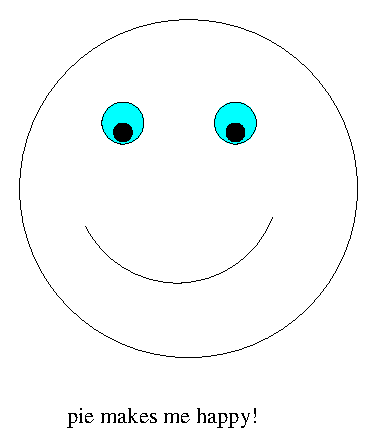
\includegraphics[width=0.4\textwidth]{fig.eps}
    \caption[Happy Face: figure example.]{\label{fig:happy} This is a figure of
      a happy face with a \texttt{psfrag} replacement.  The original figure
      (drawn in xfig and exported to a .eps file) has the text ``pie makes me
      happy!''.  The \texttt{psfrag} package replaces this with ``$\pi$ makes me
      happy!''.  Note: the Makefile compiles the sample using pdf\LaTeX\ which
      cannot use \texttt{psfrag} directly.  For some options that work with
      pdf\LaTeX, please see this discussion:
      \url{http://tex.stackexchange.com/questions/11839}.  For the caption, we
      have used the optional argument for the caption command so that only a
      short version of this caption occurs in the list of figures.}
  \end{center}
\end{figure}
\afterpage{\clearpage}
Here is an example of a figure environment.
Perhaps I should say that the example of a figure can be seen in
Figure~\ref{fig:happy}.  Figure placement can be tricky with \LaTeX\
because figures and tables are treated as ``floats'': text can flow
around them, but if there is not enough space, they will appear later.
To prevent figures from going too far, the
\verb|\afterpage{\clearpage}| command can be used.  This makes sure
that the figure are typeset at the end of the page (possibly appear on
their own on the following pages) and before any subsequent text.

The \verb|\clearpage| forces a page break so that the figure can be
placed, but without the the \verb|\afterpage{}| command, the page
would be broken too early (at the \verb|\clearpage| statement).  The
\verb|\afterpage{}| command tells \LaTeX{} to issue the command after
the present page has been rendered.

\section{Tables}
We have already included one table:~\ref{tab:Table1}.  Another table
is plopped right here.
\begin{table}[ht]
  \begin{center}
    \begin{tabular}{|l||l|l||l|l|}
      \hline
      &\multicolumn{2}{l|}{Singular}&\multicolumn{2}{l|}{Plural}\\
      \cline{2-5}
       &English&\textbf{Gaeilge}&English&\textbf{Gaeilge}\\
      \hline\hline
      1st Person&at me&\textbf{agam}&at us&\textbf{againn}\\
      2nd Person&at you&\textbf{agat}&at you&\textbf{agaibh}\\
      3rd Person&at him&\textbf{aige}&at them&\textbf{acu}\\
       &at her&\textbf{aici}& & \\
      \hline
    \end{tabular}
    \caption{
      \label{tab:Table2}
      Another table.}
  \end{center}
\end{table}
Well, actually, as with Figures, tables do not
necessarily appear right ``here'' because tables are also ``floats''.
\LaTeX{} puts them where it can.  Because of this, one should refer to
floats by their labels rather than by their location.  This example is
demonstrated by Table~\ref{tab:Table2}.  This one is pretty close,
however.  (Note: you should generally not put tables or figures in the
middle of a paragraph.  This example is for demonstration purposes
only.)

Another useful package is \verb|\usepackage{longtable}| which provides
the \texttt{longtable} environment.  This is nice because it allows
tables to span multiple pages.  Table~\ref{tab:longtable} has been
formatted this way.
\begin{center}
  \begin{longtable}{|l|l|l|}
    \caption{\label{tab:longtable}Feasible triples for 
      highly variable Grid}\\

    \hline \multicolumn{1}{|c|}{\textbf{Time (s)}} &
    \multicolumn{1}{c|}{\textbf{Triple chosen}} &
    \multicolumn{1}{c|}{\textbf{Other feasible triples}} \\ \hline
    \endfirsthead
    
    \multicolumn{3}{c}%
    {{\bfseries \tablename\ \thetable{} -- continued from previous page}} \\
    \hline \multicolumn{1}{|c|}{\textbf{Time (s)}} &
    \multicolumn{1}{c|}{\textbf{Triple chosen}} &
    \multicolumn{1}{c|}{\textbf{Other feasible triples}} \\ \hline
    \endhead
    
    \hline \multicolumn{3}{|r|}{{Continued on next page}} \\ \hline
    \endfoot

    \hline \hline
    \endlastfoot

    0 & (1, 11, 13725) & (1, 12, 10980), (1, 13, 8235), (2, 2, 0), (3, 1, 0) \\
    274 & (1, 12, 10980) & (1, 13, 8235), (2, 2, 0), (2, 3, 0), (3, 1, 0) \\
    5490 & (1, 12, 13725) & (2, 2, 2745), (2, 3, 0), (3, 1, 0) \\
    8235 & (1, 12, 16470) & (1, 13, 13725), (2, 2, 2745), (2, 3, 0), (3, 1, 0) \\
    10980 & (1, 12, 16470) & (1, 13, 13725), (2, 2, 2745), (2, 3, 0), (3, 1, 0) \\
    13725 & (1, 12, 16470) & (1, 13, 13725), (2, 2, 2745), (2, 3, 0), (3, 1, 0) \\
    16470 & (1, 13, 16470) & (2, 2, 2745), (2, 3, 0), (3, 1, 0) \\
    19215 & (1, 12, 16470) & (1, 13, 13725), (2, 2, 2745), (2, 3, 0), (3, 1, 0) \\
    21960 & (1, 12, 16470) & (1, 13, 13725), (2, 2, 2745), (2, 3, 0), (3, 1, 0) \\
    24705 & (1, 12, 16470) & (1, 13, 13725), (2, 2, 2745), (2, 3, 0), (3, 1, 0) \\
    27450 & (1, 12, 16470) & (1, 13, 13725), (2, 2, 2745), (2, 3, 0), (3, 1, 0) \\
    30195 & (2, 2, 2745) & (2, 3, 0), (3, 1, 0) \\
    32940 & (1, 13, 16470) & (2, 2, 2745), (2, 3, 0), (3, 1, 0) \\
    35685 & (1, 13, 13725) & (2, 2, 2745), (2, 3, 0), (3, 1, 0) \\
    38430 & (1, 13, 10980) & (2, 2, 2745), (2, 3, 0), (3, 1, 0) \\
    41175 & (1, 12, 13725) & (1, 13, 10980), (2, 2, 2745), (2, 3, 0), (3, 1, 0) \\
    43920 & (1, 13, 10980) & (2, 2, 2745), (2, 3, 0), (3, 1, 0) \\
    46665 & (2, 2, 2745) & (2, 3, 0), (3, 1, 0) \\
    49410 & (2, 2, 2745) & (2, 3, 0), (3, 1, 0) \\
    52155 & (1, 12, 16470) & (1, 13, 13725), (2, 2, 2745), (2, 3, 0), (3, 1, 0) \\
    54900 & (1, 13, 13725) & (2, 2, 2745), (2, 3, 0), (3, 1, 0) \\
    57645 & (1, 13, 13725) & (2, 2, 2745), (2, 3, 0), (3, 1, 0) \\
    60390 & (1, 12, 13725) & (2, 2, 2745), (2, 3, 0), (3, 1, 0) \\
    63135 & (1, 13, 16470) & (2, 2, 2745), (2, 3, 0), (3, 1, 0) \\
    65880 & (1, 13, 16470) & (2, 2, 2745), (2, 3, 0), (3, 1, 0) \\
    68625 & (2, 2, 2745) & (2, 3, 0), (3, 1, 0) \\
    71370 & (1, 13, 13725) & (2, 2, 2745), (2, 3, 0), (3, 1, 0) \\
    74115 & (1, 12, 13725) & (2, 2, 2745), (2, 3, 0), (3, 1, 0) \\
    76860 & (1, 13, 13725) & (2, 2, 2745), (2, 3, 0), (3, 1, 0) \\
    79605 & (1, 13, 13725) & (2, 2, 2745), (2, 3, 0), (3, 1, 0) \\
    82350 & (1, 12, 13725) & (2, 2, 2745), (2, 3, 0), (3, 1, 0) \\
    85095 & (1, 12, 13725) & (1, 13, 10980), (2, 2, 2745), (2, 3, 0), (3, 1, 0) \\
    87840 & (1, 13, 16470) & (2, 2, 2745), (2, 3, 0), (3, 1, 0) \\
    90585 & (1, 13, 16470) & (2, 2, 2745), (2, 3, 0), (3, 1, 0) \\
    93330 & (1, 13, 13725) & (2, 2, 2745), (2, 3, 0), (3, 1, 0) \\
    96075 & (1, 13, 16470) & (2, 2, 2745), (2, 3, 0), (3, 1, 0) \\
    98820 & (1, 13, 16470) & (2, 2, 2745), (2, 3, 0), (3, 1, 0) \\
    101565 & (1, 13, 13725) & (2, 2, 2745), (2, 3, 0), (3, 1, 0) \\
    104310 & (1, 13, 16470) & (2, 2, 2745), (2, 3, 0), (3, 1, 0) \\
    107055 & (1, 13, 13725) & (2, 2, 2745), (2, 3, 0), (3, 1, 0) \\
    109800 & (1, 13, 13725) & (2, 2, 2745), (2, 3, 0), (3, 1, 0) \\
    112545 & (1, 12, 16470) & (1, 13, 13725), (2, 2, 2745), (2, 3, 0), (3, 1, 0) \\
    115290 & (1, 13, 16470) & (2, 2, 2745), (2, 3, 0), (3, 1, 0) \\
    118035 & (1, 13, 13725) & (2, 2, 2745), (2, 3, 0), (3, 1, 0) \\
    120780 & (1, 13, 16470) & (2, 2, 2745), (2, 3, 0), (3, 1, 0) \\
    123525 & (1, 13, 13725) & (2, 2, 2745), (2, 3, 0), (3, 1, 0) \\
    126270 & (1, 12, 16470) & (1, 13, 13725), (2, 2, 2745), (2, 3, 0), (3, 1, 0) \\
    129015 & (2, 2, 2745) & (2, 3, 0), (3, 1, 0) \\
    131760 & (2, 2, 2745) & (2, 3, 0), (3, 1, 0) \\
    134505 & (1, 13, 16470) & (2, 2, 2745), (2, 3, 0), (3, 1, 0) \\
    137250 & (1, 13, 13725) & (2, 2, 2745), (2, 3, 0), (3, 1, 0) \\
    139995 & (2, 2, 2745) & (2, 3, 0), (3, 1, 0) \\
    142740 & (2, 2, 2745) & (2, 3, 0), (3, 1, 0) \\
    145485 & (1, 12, 16470) & (1, 13, 13725), (2, 2, 2745), (2, 3, 0), (3, 1, 0) \\
    148230 & (2, 2, 2745) & (2, 3, 0), (3, 1, 0) \\
    150975 & (1, 13, 16470) & (2, 2, 2745), (2, 3, 0), (3, 1, 0) \\
    153720 & (1, 12, 13725) & (2, 2, 2745), (2, 3, 0), (3, 1, 0) \\
    156465 & (1, 13, 13725) & (2, 2, 2745), (2, 3, 0), (3, 1, 0) \\
    159210 & (1, 13, 13725) & (2, 2, 2745), (2, 3, 0), (3, 1, 0) \\
    161955 & (1, 13, 16470) & (2, 2, 2745), (2, 3, 0), (3, 1, 0) \\
    164700 & (1, 13, 13725) & (2, 2, 2745), (2, 3, 0), (3, 1, 0) \\
\end{longtable}
\end{center}

\subsection*{An Unnumbered Subsection}
Note that if you use subsections or further divisions under an
unnumbered section, then you should make them unnumbered as well
otherwise you will end up with zeros in the section numbering.

\chapter{Landscape Mode}
The landscape mode allows you to rotate a page through 90 degrees.  It
is generally not a good idea to make the chapter heading landscape,
but it can be useful for long tables etc.

\begin{landscape}
  This text should appear rotated, allowing for formatting of very
  wide tables etc.  Note that this might only work after you convert
  the \texttt{dvi} file to a postscript (\texttt{ps}) or \texttt{pdf}
  file using \texttt{dvips} or \texttt{dvipdf} etc.  This feature is
  provided by the \verb|lscape| and the \verb|pdflscape| packages.
  The latter is preferred if it works as it also rotates the pages in
  the pdf file for easier viewing.
\end{landscape}

%%% This file is setup to use a bibtex file sample.bib and uses the
%%% plain style.  Other styles may be used depending on the conventions
%%% of your field of study.
%%%
%%%% Note: the bibliography must come before the appendices.
\bibliographystyle{plain}
\bibliography{sample}

%%% Use this to reset the appendix counter.  Note that the FoGS
%%% requires that the word ``Appendices'' appear in the table of
%%% contents either before each appendix lable or as a division
%%% denoting the start of the appendices.  We take the latter option
%%% here.  This is ensured by making the \texttt{appendicestoc} option
%%% a default option to the UBC thesis class.

%%%% If you only have one appendix, please uncomment the following line.
%% \renewcommand{\appendicesname}{Appendix}
\appendix
\chapter{First Appendix}
Here you can have your appendices.  Note that if you only have a
single appendix, you should issue
\verb|\renewcommand{\appendicesname}{Appendix}| before calling
\verb|\appendix| to display the singular ``Appendix'' rather than the
default plural ``Appendices''.

\chapter{Second Appendix}
Here is the second appendix.

%%% This changes the headings and chapter titles (no numbers for
%%% example).
\backmatter

%%% Indices come here if you have them.


\chapter*{Additional Information}
This chapter shows you how to include additional information in your
thesis, the removal of which will not affect the submission.  Such
material should be removed before the thesis is actually submitted.

First, the chapter is unnumbered and not included in the Table of
Contents.  Second, it is the last section of the thesis, so its
removal will not alter any of the page numbering etc. for the previous
sections.  Do not include any floats, however, as these will appear in
the initial lists.

The \texttt{ubcthesis} \LaTeX{} class has been designed to aid you in
producing a thesis that conforms to the requirements of The
University of British Columbia Faculty of Graduate Studies (FoGS).

Proper use of this class and sample is highly recommended---and should
produce a well formatted document that meets the FoGS requirement.
Notwithstanding, complex theses may require additional formatting that
may conflict with some of the requirements.  We therefore \emph{highly
  recommend} that you consult one of the FoGS staff for assistance and
an assessment of potential problems \emph{before} starting final
draft.

While we have attemped to address most of the thesis formatting
requirements in these files, they do not constitute an official set of
thesis requirements.  The official requirements are available at the
following section of the FoGS web site:
\begin{center}
  \begin{tabular}{|l|}
    \hline
    \url{http://www.grad.ubc.ca/current-students/dissertation-thesis-preparation}\\
    \hline
  \end{tabular}
\end{center}
We recommend that you review these instructions carefully.

%    \end{macrocode}
% \subsection{End of Document}
%    \begin{macrocode}
\end{document}
%    \end{macrocode}
%    Finally, we close off the file so that nothing else is put
%    into the sample thesis.
%    \begin{macrocode}
%</ubcsampletex>
%    \end{macrocode}
%
% \changes{v1.65}{2010/05/05}{Add the hyperref option linktocpage as a
%   default and added more comments about this package.}
% \section{Sample MIT Thesis}
%
%    This was a thesis conforming to the Massachusetts Institute of
%    Technology guidelines when I was a student.  I have not kept on
%    top of the changes, so some modifications may have to be made.
%
%    Here is the comment that tells \prog{docstrip} to put the
%    following code into \file{mitsample.tex}.
%
%    \begin{macrocode}
%<*mitsampletex>
%    \end{macrocode}
% 
% \subsection{Identification}
%    This section identifies the version of the file.  It
%    also indicates which version of \LaTeX{} (\LaTeXe) is required and
%    makes sure that an appropriate message is displayed when another \TeX{}
%    format is used.
%    \begin{macrocode}
%% This Sample thesis requires \LaTeX2e
\NeedsTeXFormat{LaTeX2e}[1995/12/01]
%    \end{macrocode}
%
%    Now we announce the file or class name and its version:
%
% \iffalse VERSION \fi
%    \begin{macrocode}
\ProvidesFile{mitsample.tex}[2012/04/07 v1.70 ^^J
 Massachusetts Institute of Technology Sample Thesis]
%    \end{macrocode}
%
% \subsection{Document Structure}
%    This section describes the structure that your \LaTeX{} document must
%    have.  Various sections of the sample code will be presented to
%    illustrate this structure though the sample file \file{mitsample.tex}
%    does not contain all of the options and features.
%
%    The first section of a \LaTeX{} document contains information
%    about the structure of the document.  This is called the document
%    preamble.
%
%    Usually the first command is the |\documentclass| command which
%    specifies the class to use and the options to the class 
%
%    \begin{macrocode}

\documentclass[msc,10pt,oneside]{mitthesis}
%    \end{macrocode}
%
%    \begin{macrocode}
%%
%% To compile issue the following commands:
%% latex mitsample
%% bibtex mitsample
%% latex mitsample
%% latex mitsample
%% latex mitsample
%%
%% To view use xdvi (on unix systems):
%% xdvi mitsample.dvi
%%
%% To make a postscript file, use dvips:
%% dvips -o mitsample.ps mitsample.dvi
%%
%% To view the postscript file, use ghostview or gv (on unix systems):
%% gv mitsample.ps
%%
%%************************************************
%% Optional packages.
%%
%% The use of these packages is optional: they are standard now and
%% should be installed on your system, but if they are not, you might
%% have to comment out the appropriate lines to get this file to
%% compile.
%%
%%******** natbib ********************************
%% This is a very nice package for bibliographies.  It includes options
%% for sorting and compressing bibliographic entries.
\usepackage[numbers,sort&compress]{natbib}

%%******** graphics and graphicx ******************************
%% This allows you to include encapsulated postscript files.  If you
%% don't have this, comment the \includegraphics{} line following the
%% comment "%includegraphics" later in this file.
\usepackage{graphicx}

%%******** pdflscape ********************************
%% This allows you to include landscape layout pages by using the
%% |landscape| environment.  The use of |pdflscape| is preferred over
%% the standard |lscape| package because it automatically rotates the
%% page in the pdf file for easier reading.  (Thanks to Joseph Shea
%% for pointing this out.)
\usepackage{pdflscape}

%%******** psfrag ******************************
%% This allows you to replace text in postscript pictures with formated
%% latex text.  This allows you to use math in graph labels
%% etc. Uncomment the psfrag lines following the "%psfrag" comment
%% later in this file if you don't have this package.  The replacements
%% will only be visible in the final postscript file: they will be
%% listed in the .dvi file but not performed.
\usepackage{psfrag}

%%******** afterpage ***************************
%% This package allows you to issue commands at the end of the current
%% page.  A good use for this is to use the command
%% \afterpage{\clearpage} right after a figure.  This will cause the
%% figure to be inserted on the page following the current one (or on
%% the current page if it will fit) but will not break the page in the
%% middle.
\usepackage{afterpage}

%%******** hyperref *****************************
%% Please read the manual:
%% http://www.tug.org/applications/hyperref/manual.html
%%
%% This adds hyperlinks to your document: with the right viewers (later
%% versions of xdvi, acrobat with pdftex, latex2html etc.) this will
%% make your equation, figure, citation references etc. hyperlinks so
%% that you can click on them.  Also, your table of contents will be
%% able to take you to the appropriate sections.  In the viewers that
%% support this, the links often appear with an underscore.  This
%% underscore will not appear in printed versions.
%%
%% Note: if you do not use the hypertex option, then the dvips driver
%% may be loaded by default.  This will cause the entries in the list
%% of figures and list of tables to be on a single line because dvips
%% does not deal with hyperlinks on broken lines properly.
%%
%% NOTE: HYPERREF is sensitive to the ORDER in which it is LOADED.
%% For example, it must be loaded AFTER natbib but BEFORE newly
%% defined float environments.  See the README file with the hyperref
%% for some help with this.  If you have some very obscure errors, try
%% first disabling hyperref.  If that fixes the problem, try various
%% orderings.
%%
%% Note also that there is a bug with versions before 2003/11/30
%% v6.74m that cause the float package to not function correctly.
%% Please ensure you have a current version of this package.  A
%% warning will be issued if you leave the date below but do not have
%% a current version installed.
%%
%% Some notes on options: depending on how you build your files, you
%% may need to choose the appropriate option (such as [pdftex]) for the
%% backend driver (see the hyperref manual for a complete list).  Also,
%% the default here is to make links from the page numbers in the table
%% of contents and lists of figures etc.  There are other options:
%% excluding the [linktocpage] option will make the entire text a
%% hyperref, but for some backends will prevent the text from wrapping
%% which can look terrible.  There is a [breaklinks=true] option that
%% will be set if the backend supports (dvipdfm for example supports
%% it but does not work with psfrag.)
%%
%% Finally, there are many options for choosing the colours of the
%% links.  These will be included by default in future versions but
%% you should probably consider changing some now for the electronic
%% version of your thesis.
\usepackage[unicode=true,
  linktocpage,
  linkbordercolor={0.5 0.5 1},
  citebordercolor={0.5 1 0.5},
  linkcolor=blue]{hyperref}

%% If you would like to compile this sample thesis without the
%% hyperref package, then you will need to comment out the previous
%% \usepackage command and uncomment the following command which will
%% put the URL's in a typewriter font but not link them.
%%\newcommand\url[1]{\texttt{#1}}

%% These commands are optional.  The defaults are shown.
\institution{Massachusetts Institute of Technology}
\institutionaddress{Cambridge}
\program{Physics}

%% You can issue as many of these as you have...
\previousdegree{B.Sc., The University of British Columbia, 1999}
\previousdegree{M.Sc., The University of British Columbia, 2001}

%% You can override the option setting here.
%% \degreetitle{Jack of All Trades}

%% These commands are required.
\title{A Sample Thesis}
\subtitle{With a Subtitle}
\author{Michael M$^{\rm c}$Neil Forbes}
\copyrightyear{2000}
\submitdate{June 2004}

%% These commands are required by MIT.
\advisor{Frank Wilczek}
\advisortitle{Herman Feshbach Professor of Physics}
\chairman{Thomas Greytak}{Professor and Associate Department Head for
  Education}
%    \end{macrocode}
%
% \subsubsection{Chapter and section counter formats}
%    For any counter \Lcount{CTR}, |\theCTR| is a macro that defines
%    the printed version of counter \Lcount{CTR}.  It is defined in
%    terms of the following macros:
%
%    |\arabic{|\Lcount{COUNTER}|}| prints the value of
%    \Lcount{COUNTER} as an Arabic numeral.
%
%    |\roman{|\Lcount{COUNTER}|}| prints the value of
%    \Lcount{COUNTER} as a lowercase Roman numeral.
%
%    |\Roman{|\Lcount{COUNTER}|}| prints the value of
%    \Lcount{COUNTER} as an uppercase Roman numeral.
%
%    |\alph{|\Lcount{COUNTER}|}| prints the value of \Lcount{COUNTER}
%    as a lowercase letter: $1 =$~a, $2 =$~ b, etc.
%
%    |\Alph{|\Lcount{COUNTER}|}| prints the value of \Lcount{COUNTER}
%    as an uppercase letter: $1 =$~A, $2 =$~B, etc.
%
%    This section of the sample class redefines these (actually, the
%    redefinitions match the defaults so this would be pointless in
%    the actual thesis, but is here for demonstration purposes.)
%    \begin{macrocode}
%% One might want to override the format of the section and chapter
%% numbers.  This shows you how to do it.  Note that 
\renewcommand\thepart         {\Roman{part}}
\renewcommand\thechapter      {\arabic{chapter}}
%    \end{macrocode}
%    The section and lower commands also display the numbers of
%    higher sections too and a punctuation mark.  These show you how
%    to change these.  (Again, the formats actually given here are the
%    defaults.)
%    \begin{macrocode}
\renewcommand\thesection      {\thechapter.\arabic{section}}
\renewcommand\thesubsection   {\thesection.\arabic{subsection}}
\renewcommand\thesubsubsection{\thesubsection.\arabic{subsubsection}}
\renewcommand\theparagraph    {\thesubsubsection.\arabic{paragraph}}
\renewcommand\thesubparagraph {\theparagraph.\arabic{subparagraph}}

% Two related counters control the level of sections that are numbered
% and the level of sections included in the table of contents:
\setcounter{tocdepth}{2}
\setcounter{secnumdepth}{2}

%% Here is the start of the document.
\begin{document}

%% Unlike the UBC thesis, page numbering for MIT theses should start
%% at 1 and continue.  Thus, there is no \frontmatter command issued
%% here as there was for the UBC thesis.

\maketitle
\authorizationform
\begin{abstract}
  The \texttt{genthesis.cls} \LaTeX{} class file and accompanying
  documents, such as this sample thesis, are distributed in the hope
  that it will be useful but without any warranty (without even the
  implied warranty of fitness for a particular purpose).  For a
  description of this file's purpose, and instructions on its use, see
  below.
  
  These files are distributed under the GPL which should be included
  here in the future.  Please let the author know of any changes or
  improvements that should be made.

  Michael Forbes.
  mforbes@alum.mit.edu
\end{abstract}

\tableofcontents
\listoftables
\listoffigures
%% Any other lists should come here, i.e.
%% Abbreviation schemes, definitions, lists of formulae, list of
%% schemes, etc.

\chapter{Preface}
These papers have been published earlier\ldots.

\chapter{Acknowledgements}
Thank you mother here.

%% Force a new page.
\newpage

%% Any other unusual sections should come here between the
%% acknowledgements and the main body. 

%% Suppress the running headers for this page only.
\thispagestyle{plain}
\chapter*{Disclaimer} % Unnumbered 
The \texttt{mitthesis} \LaTeX{} class and the accompanying sample files
are \emph{unofficial} and are not supported by the Massachusetts
Institute of Technology.  While I have attempted to make the style
file and sample files conform to all of the requirements set forth by
the library, you should always consult one of the library staff
members for assistance with problems \emph{before} starting final
draft.  You should be able to find the thesis requirements at one of
the following sites:
\begin{table}[h]
  \begin{center}
    \begin{tabular}{|l|}
      \hline
      \url{http://libraries.mit.edu/archives/thesis-specs/}\\
      \url{http://libraries.mit.edu/archives/index.html}\\
      \hline
    \end{tabular}
  \end{center}
  \caption{\label{tab:ubcurls}
    Potential sources of information regarding thesis preparation at MIT.}
\end{table}

%% Force a new page.
\newpage

%% Suppress the running headers for this page only.
\thispagestyle{plain}

%% Here we provide a short optional argument to \chapter[]{}.  This
%% optional argument will appear in the table of contents.  For long
%% titles, one should use this to give a single-line entry to the
%% table of contents.
\chapter[Poem]{A Japanese Introduction}

%% Here is a quote:
\begin{quote}
  % It is centered
  \begin{center}
    This is a small poem,\\
    a little poem, a Haiku,\\
    to show you how to.\\
    ---Michael Forbes.
  \end{center}
\end{quote}
This small poem shows several features:
\begin{itemize}
\item The \verb|\newpage| command has been used to force a page break.
\item The pagestyle has been set to suppress the headers using the
  command \verb|\thispagestyle{plain}|.  Note that using
  \verb|\pagestyle{plain}| would have affected all of the subsequent
  pages.
\item The \verb|\chapter[Poem]{A Japanese Introduction}| command has
  been used with an optional argument to generate a title and to list
  this ``chapter'' in the table of contents as ``Poem''.  If one did
  not desire to have an entry in the table of contents, then one would
  just use the starred command \verb|\chapter*{}|.  The use of an
  optional argument is useful for long chapter and section titles that
  take up too much space in the table of contents.
\end{itemize}

%% Parts are the largest units
\part{Thesis}

%% Chapters are the next main unit.
\chapter{This is a Chapter}

%% Sections are a sub-unit
\section{A Section}
Here is a section with some text.  Equations look like this $y=x$.

This is an example of a second paragraph in a section so you can
see how much it is indented by.

%% Subsections follow
\subsection{This is a Subsection}
Here is an example of a citation: \cite{Forbes:2006ba}.  The actual
form of the citation is governed by the bibliographystyle.  These
citations are maintained in a BIBTeX file \texttt{sample.bib}.  You
could type these directly into the file.  For an example of the format
to use look at the file \texttt{mitsample.bbl} after you compile this
file.

This is an example of a second paragraph in a subsection so you can
see how much it is indented by.

\subsubsection{This is a Subsubsection}
Here are some more citations \cite{LL3:1977,Peccei:1989,Turner:1999}.
If you use the \texttt{natbib} package with the \verb+sort&compress+
option, then the following citation will look the same as the first
citation in this section: \cite{Turner:1999,Peccei:1989,LL3:1977}.

This is an example of a second paragraph in a subsubsection so you can
see how much it is indented by.

\paragraph{This is a Paragraph}
Paragraphs and subparagraphs are the smallest units of text.  There is
no subsubsubsection etc.

\subparagraph{This is a Subparagraph}
This is the last level of organisation.  If you need more than this,
you should consider reorganizing your work\dots

\begin{equation}
  \mathrm{f}(x)=\int_{-\infty}^{\int_{-\infty}^x 
    e^{-\frac{y^2}{2}}\mathrm{d}{y}}e^{-z^2}\mathrm{d}z
\end{equation}

In order to show you what a separate page would look like (i.e. without
a chapter heading) I must type some more text.  Thus I will babble a
bit and keep babbling for at least one more page\ldots  What you
should notice is that the chapter titles appear substantially lower
than the continuing text. Babble babble
babble babble babble babble babble babble babble babble babble babble
babble babble babble babble babble babble babble babble babble babble
babble babble babble babble babble babble babble babble babble babble
babble babble babble babble babble babble babble babble babble.

Babble babble babble babble babble babble babble babble babble babble
babble babble babble babble babble babble babble babble babble babble
babble babble babble babble babble babble babble babble babble babble
babble babble babble babble babble babble babble babble babble babble
babble babble babble babble babble babble babble babble babble babble
babble babble babble babble babble babble babble babble babble babble
babble babble babble babble babble babble babble babble babble babble
babble babble babble babble babble babble babble babble babble babble
babble babble babble babble babble babble babble babble babble babble
babble babble babble babble babble babble babble babble babble babble
babble babble babble babble babble babble babble babble babble babble
babble babble babble babble babble babble babble babble babble babble
babble babble babble babble.

\begin{table}[t]                 %optional [t, b or h];
  \begin{tabular}{|r||r@{.}l|}
    \hline
    Phoenix & \$960&35\\
    \hline
    Calgary & \$250&00\\
    \hline
  \end{tabular}
  \caption{
    \label{tab:Table1}
    Here is the caption for this wonderful table.Text of Caption}
\end{table}

\chapter[Another Chapter\ldots]{Another Chapter with a Very Long
  Chapter-name that will Probably Cause Problems}
This chapter name is very long and does not display properly in the
running headers or in the table of contents.  To deal with this, we
provide a shorter version of the title as the optional argument to the
\verb|\chapter[]{}| command.

\section{Another Section}
Another bunch of text to demonstrate what this file does.
You might want a list for example:
\begin{itemize}
\item An item in a list.
\item Another item in a list.
\end{itemize}

\section*{An Unnumbered Section That is Not Included in the Table of
  Contents}
%%% We would like to place the figure here, so we start with [h].
%%% Note that we have located the figure between paragraphs (rather,
%%% before one) so that it does not split up sentences.
\begin{figure}[ht]
  \begin{center}
%%% psfrag: comment the following line if not using the psfrag package
    \psfrag{pie makes me happy!}{$\pi$ makes me happy!}
%%% includegraphics: comment the following if not using the graphicx package
    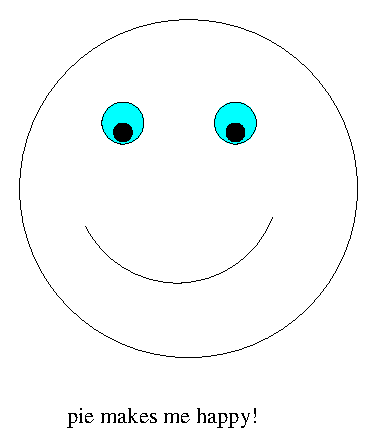
\includegraphics[width=0.4\textwidth]{fig.eps}
    \caption[Happy Face: figure example.]{\label{fig:happy} This is a
      figure of a happy face with a \texttt{psfrag} replacement.  The
      original figure (drawn in xfig and exported to a .eps file) has
      the text ``pie makes me happy!''.  The \texttt{psfrag} package
      replaces this with ``$\pi$ makes me happy!''.  Note that we have
      used the optional argument for the caption command so that only
      a short version of this caption occurs in the list of figures.}
  \end{center}
\end{figure}
\afterpage{\clearpage}
Here is an example of a figure environment.
Perhaps I should say that the example of a figure can be seen in
Figure~\ref{fig:happy}.  Figure placement can be tricky with \LaTeX\
because figures and tables are treated as ``floats'': text can flow
around them, but if there is not enough space, they will appear later.
To prevent figures from going too far, the
\verb|\afterpage{\clearpage}| command can be used.  This makes sure
that the figure are typeset at the end of the page (possibly appear on
their own on the following pages) and before any subsequent text.

The \verb|\clearpage| forces a page break so that the figure can be
placed, but without the the \verb|\afterpage{}| command, the page
would be broken too early (at the \verb|\clearpage| statement).  The
\verb|\afterpage{}| command tells \LaTeX{} to issue the command after
the present page has been rendered.

Be careful when using the ``here'' placement option
\verb|\begin{figure}[ht]| that you place the figure between paragraphs
in your text, otherwise \LaTeX{} might actually insert it in the
middle of a sentence (which does not look very good and is frowned
upon by the editors!)

\subsection*{An Unnumbered Subsection}
Note that if you use subsections or further divisions under an
unnumbered section, then you should make them unnumbered as well
otherwise you will end up with zeros in the section numbering.

\chapter{Landscape Mode}
The landscape mode allows you to rotate a page through 90 degrees.  It
is generally not a good idea to make the chapter heading landscape,
but it can be useful for long tables etc.

\begin{landscape}
  This text should appear rotated, allowing for formatting of very
  wide tables etc.  Note that this might only work after you convert
  the \texttt{dvi} file to a postscript (\texttt{ps}) or \texttt{pdf}
  file using \texttt{dvips} or \texttt{dvipdf} etc.  This feature is
  provided by the \verb|lscape| and the \verb|pdflscape| packages.
  The latter is preferred if it works as it also rotates the pages in
  the pdf file for easier viewing.
\end{landscape}

%% This file is setup to use a bibtex file sample.bib and uses the
%% plain style.  Note, the bibliography could come after the appendices.
\bibliographystyle{plain}
\bibliography{sample}

%% If you only have one appendix, please uncomment the following line.
% \renewcommand{\appendicesname}{Appendix}
\appendix
\chapter{First Appendix}
Here you can have your appendices.  Note that if you only have a
single appendix, you should issue
\verb|\renewcommand{\appendicesname}{Appendix}| before calling
\verb|\appendix| to display the singular ``Appendix'' rather than the
default plural ``Appendices''.

\chapter{Second Appendix}
Here is the second appendix.

%%% This changes the headings and chapter titles (no numbers for
%%% example).
\backmatter

%% Indices come here.

%    \end{macrocode}
% \subsection{End of Document}
%    \begin{macrocode}
\end{document}
%    \end{macrocode}
%    Finally, we close off the file so that nothing else is put
%    into the sample thesis.
%    \begin{macrocode}
%</mitsampletex>
%    \end{macrocode}
%
% \section{Sample Bibliographic Database (BIBTeX)}
%
%    This section presents the code for the bibliographic database for
%    the sample thesis with comments. It is recommended that you first
%    obtain the sample thesis files and compile them as described in
%    Section~\ref{sec:GettingStartedSampleThesis}.  This way you can try
%    the various options to see how they work.
%
%    Here is the comment that tells \prog{docstrip} to put the
%    following code into \file{sample.bib}.
%
%    \begin{macrocode}
%<*samplebib>
%    \end{macrocode}
% 
% \subsection{Identification}
%    This section identifies the version of the file.  Formally this
%    should be a comment, but as it appears prior to any entry, bibtex
%    will treat it as a comment (beware though, the character \@ may
%    not appear outside of an entry.)
%
% \iffalse VERSION \fi
%    \begin{macrocode}
\ProvidesFile{sample.bib}[2012/04/07 v1.70 ^^J
University of British Columbia Sample Thesis]
%    \end{macrocode}
%
% \subsection{Document Structure}
%    \begin{macrocode}
%% These are just some examples of articles and books.  Some of the fields
%% are not needed, for example the abstract and SLACcitation fields.  There
%% are many other types of documents.  The entry CL:2000 poses a problem 
%% in the URL field.  I am not sure how to get around this right now.

@Article{Apple:2010,
  author =       {Michael McNeil Forbes and A. Apple and B. Boat},
  title =        {Frequency of Quality Testing in Syrup Creation},
  journal =      "Maple Science J.",
  volume =       {255},
  year =         {2010},
  pages =        {139--144},
}

@Article{Forbes:2006ba,
     author    = "Forbes, Michael McNeil and Zhitnitsky, Ariel R.",
     title     = "{Dark antimatter as a galactic heater: X-rays from the core
                  of our  galaxy}",
     journal   = "JCAP",
     volume    = "0801",
     year      = "2008",
     pages     = "023",
     eprint    = "astro-ph/0611506",
     SLACcitation  = "%%CITATION = ASTRO-PH/0611506;%%",
     abstract  = {Several independent observations of the Galactic
       core suggest hitherto unexplained sources of energy.  We
       suggest that dark matter in the form of dense antimatter
       nuggets could provide a natural site for electron and proton
       annihilation, providing 511 {keV} photons, gamma-rays, and
       diffuse {keV} X-ray radiation.  We show that identifying dark
       matter as antimatter nuggets is consistent with the observed
       emissions, and we make definite predictions about their
       spectrum and morphology.  If correct, our proposal not only
       identifies dark matter and explains baryogenesis, but allows
       X-ray observations to directly probe the matter
       distribution in our Galaxy.}
}

@Book{LL3:1977,
  author       = "L. D. Landau and E. M. Lifshitz",
  title        = "Quantum Mechanics: Non-relativistic theory",
  publisher    = "Pergamon Press",
  year         = "1989, c1977",
  volume       = "3",
  series       = "Course of Theoretical Physics",
  address      = "Oxford; New York",
  edition      = "Third",
}


@InCollection{Peccei:1989,
  author       = "R. D. Peccei",
  title        = "Special Topics: The Strong {CP} Problem",
  booktitle    = "CP violation",
  publisher    = "World Scientific",
  year         = "1989",
  editor       = "C. Jarlskog",
  address      = "Singapore",
  month        = jan,
}

@Article{Bulgac:2006gh,
  author =       {Aurel Bulgac and Michael McNeil Forbes and Achim
                  Schwenk},
  title =        {Induced {P-wave} Superfluidity in Asymmetric Fermi
                  Gases},
  journal =      "Phys. Rev. Lett.",
  volume =       97,
  year =         2006,
  pages =        020402,
  eprint =       {arXiv:cond-mat/0602274},
  SLACcitation = "%%CITATION = COND-MAT 0602274;%%",
  abstract =     {We show that two new intra-species P-wave superfluid
                  phases appear in two-component asymmetric Fermi
                  systems with short-range {S-wave} interactions. In
                  the {BEC} limit, phonons of the molecular {BEC}
                  induce {P-wave} superfluidity in the excess
                  fermions. In the {BCS} limit, density fluctuations
                  induce {P-wave} superfluidity in both the majority
                  and the minority species. These phases may be
                  realized in experiments with spin-polarized Fermi
                  gases.}
}

@InProceedings{CL:2000,
  author       = "S. A. {Colgate} and H. {Li}",
  title        = "The Magnetic Fields of the Universe and Their Origin",
  booktitle    = "10 pages, 1 figure (figures.png), invited talk at IAU
                 195 Preprint no. LAUR 00-180.",
  year         = "2000",
  month        = jan,
  pages        = "1418",
  URL          = "{http://adsabs.harvard.edu/cgi-bin/nph-bib_query?bibcode=\
2000astro.ph..1418C&db_key=PRE}",
  adsnote      = "Provided by the NASA Astrophysics Data System",
  eprint       = "astro-ph/0001418",
  abstract     = "Recent rotation measure observations of a dozen or so
                 galaxy clusters have revealed a surprisingly large
                 amount of magnetic fields, whose estimated energy and
                 flux are, on average, {$\sim 10^{58}$} ergs and {$\sim
                 10^{41}$ G cm$^2$}, respectively. These quantities are
                 so much larger than any coherent sums of individual
                 galaxies within the cluster that an efficient galactic
                 dynamo is required. We associate these fields with
                 single AGNs within the cluster and therefore with all
                 galaxies during their AGN phase. Only the central,
                 massive black hole (BH) has the necessary binding
                 energy, {$\sim 10^{61}$} ergs. Only the accretion disk
                 during the {BH} formation has the winding number,
                 {$\sim 10^{11}$} turns, necessary to make the gain and
                 magnetic flux. We present a model of the BH accretion
                 disk dynamo that might create these magnetic fields,
                 where the helicity of the {$\alpha - \Omega$} dynamo is
                 driven by star-disk collisions. The back reaction of
                 the saturated dynamo forms a force-free field helix
                 that carries the energy and flux of the dynamo and
                 redistributes them within the clusters.",
}

@Misc{Turner:1999,
  author       = "M. S. Turner",
  title        = "Dark Matter, Dark Energy and Fundamental Physics",
  howpublished = "astro-ph/9912211",
  year         = "1999",
  month        = dec,
  abstract     = "More than sixty years ago Zwicky made the case that
                 the great clusters of galaxies are held together by the
                 gravitational force of unseen (dark) matter. Today, the
                 case is stronger and more precise: Dark, nonbaryonic
                 matter accounts for {$30\% \pm 7\%$} of the critical mass
                 density, with baryons (most of which are dark)
                 contributing only {$4.5\% \pm 0.5\%$} of the critical
                 density. The large-scale structure that exists in the
                 Universe indicates that the bulk of the nonbaryonic
                 dark matter must be cold (slowly moving particles). The
                 SuperKamiokande detection of neutrino oscillations
                 shows that particle dark matter exists, crossing an
                 important threshold. Over the past few years a case has
                 developed for a dark-energy problem. This dark
                 component contributes about {$80\% \pm 20\%$} of the critical
                 density and is characterized by very negative pressure
                 {$(p_X < -0.6 \rho_X)$}. Consistent with this picture of
                 dark energy and dark matter are measurements of {CMB}
                 anisotropy that indicate that total contribution of
                 matter and energy is within {$10\%$} of the critical
                 density. Fundamental physics beyond the standard model
                 is implicated in both the dark matter and dark energy
                 puzzles: new fundamental particles (e.g., axion or
                 neutralino) and new forms of relativistic energy (e.g.,
                 vacuum energy or a light scalar field). A flood of
                 observations will shed light on the dark side of the
                 Universe over the next two decades; as it does it will
                 advance our understanding of the Universe and the laws
                 of physics that govern it.",
}

@Book{Vilenkin:1994,
  author =       {Alexander Vilenkin and E. P. S. Shellard},
  title =        {Cosmic Stringas and Other Topological Defects},
  publisher =    {Cambridge University Press},
  year =         1994,
  address =      {Cambridge}
}

%</samplebib>
%    \end{macrocode}
%
% \part[The \file{genthesis} Document Class: For thesis class maintainers]%
%      {The \file{genthesis} Document Class}
%
%    Here starts the description of the actual thesis class
%    definitions. All of the source code is documented here.  This is
%    generally not intended to be of use to people writing theses
%    unless they need to know the internals of how the thesis class
%    works.  It may be of use to people writing other classes as I
%    have included many comments about things I learned while writing
%    the class.  We start with some notes about this.
%
% \section{Notes about Writing Classes}
%
%    My philosophy in writing the thesis classes is described below:
%    \begin{enumerate}
%    \item The thesis class should behave as close to the standard
%      classes as possible so that it is compatible with as many other
%      packages as possible.  To this end, the thesis class has been
%      crafted directly from the standard \LaTeX\ \file{book} class.
%    \item If there is a standard way to accomplish a certain task,
%      then support that rather than reimplementing the method in a
%      non-standard way.  For example, encourage the use packages like
%      \file{fancyhdr} or \file{geometry} rather than providing a
%      bunch of thesis specific commands for specifying fancy headers
%      and for changing the margins.
%    \item Formatting options should be easily specified in both the
%      thesis flavours and actual theses.  This goal is only partly
%      realized, but many of the magic numbers that control formatting
%      in the original book class have been replaced with variables
%      that can be controlled by various options.
%    \end{enumerate}
%  
%    I based this code on the file \file{ltclass.dtx} and have kept
%    most of the change notes and comments so that one has a hope of
%    identifying potential incompatibilities and does not have to
%    reinvent the wheel.
%
%    It is important to make sure that the interface to standard
%    \LaTeX\ commands does not change.  For example, I wanted to
%    provide a customized version of |\part|, |\chapter| etc.\ such
%    that the starred form accepted an optional argument, adding a
%    line to the table of contents.  This turned out to break the
%    \file{hyperref} package because it redefines |\@chapter| and
%    assumes that this behaves the same way as in the standard \LaTeX\
%    distribution.
%
%    A similar problem with \file{hyperref} compatibility was
%    encountered when trying to add formatting options for the table
%    of contents.  I thought that it would be easiest to simply modify
%    the |\contentsline| command to include the formatting, but the
%    \file{hyperref} package relies on modifying this command to work,
%    so this type of change was incompatible.  Hopefully future
%    versions of \LaTeX\ will have much less hard-coded so these types
%    of changes are easier to make.  Now, onto the code! 
%
% \changes{v1.00d}{1993/11/30}{remove \cs{@in}, made option makeindex
%    a synonym for option makeidx}
% \changes{v1.00d}{1993/11/30}{removed \cs{@minus}, \cs{@plus},
%    \cs{@settopoint}, \cs{@setfontsize}; they are now in the
%    kernel}
% \changes{v1.00d}{1993/11/30}{Added use of \cs{NeedsTeXFormat}}
% \changes{v1.00d}{1993/11/30}{Replaced \cs{bf} with \cs{bfseries};
%    \cs{rm} with \cs{rmfamily}}
% \changes{v1.00d}{1993/11/30}{Made eqaution and eqnarray environments
%    in the fleqn option up to date with latex.dtx}
% \changes{v1.00f}{1993/12/08}{Made all lines shorter than 72 characters}
% \changes{v1.00g}{1993/12/08}{Made change in eqnarray for the fleqn
%    option, as suggested by Rainer.}
% \changes{v1.00h}{1993/12/18}{Made the definitions of the font- and
%    size-changing commands use \cs{renew} rather than \cs{new}.
%    Defined the float parameters with \cs{renewcommand} rather than
%    \cs{newcommand}.  Corrected some typos in the fleqn option.
%    Replaced two occurrences of -\cs{@secpenalty} by
%    \cs{@secpenalty}.  ASAJ.}
% \changes{v1.00j}{1993/12/20}{Added \cs{ProvidesFile} to size files}
% \changes{v1.00j}{1993/12/10}{Use \cs{cmd} in change entries}
% \changes{v1.00k}{1994/01/09}{Removed some typos/bugs}
% \changes{v1.00l}{1994/01/11}{add the extension to the names of the
%     files} 
% \changes{v1.00l}{1994/01/10}{Changed version numbering; moved leqno
%    and fleqn options to an external file.}
% \changes{v1.00n}{1994/01/19}{Removed code for makeidx option and made
%    it a separate package; removed use of \cs{setlength} from list
%    parameters.}
% \changes{v1.00o}{1994/01/31}{Small documentation changes}
% \changes{v1.00q}{1994/02/16}{Small documentation changes}
% \changes{v1.01a}{1994/03/12}{Removed \cs{typeout} messages}
% \changes{v1.01f}{1994/04/15}{Inserted forgotten line break}
% \changes{v1.02a}{1994/03/17}{Added openright option. (LL)}
% \changes{v1.02b}{1994/03/17}{Added the \ldots{}matter commands. (LL)}
% \changes{v1.02d}{1994/04/11}{Checked the file for long lines and
%    wrapped them when necessary; made a slight implementation
%    modification to the openright and openany options.}
% \changes{v1.02i}{1994/04/28}{Use LaTeX instead of LaTeX2e in messages}
% \changes{v1.02j}{1994/05/01}{Removed the use of \cs{fileversion}
%    c.s.}
% \changes{v1.02l}{1994/05/11}{changed some \cs{changes} entries}
% \changes{v1.02m}{1994/05/12}{Forgot a few entries}
% \changes{v1.02o}{1994/05/24}{Changed file information}
% \changes{v1.02p}{1994/05/27}{Moved identification and driver to the
%    front of the file}
% \changes{v1.02t}{1994/06/22}{Refrased a few sentences to prevent
%    overfull hboxes}
% \changes{v1.02v}{1994/12/01}{Made the oneside option work for the
%    book class}
% \changes{v1.02w}{1994/12/01}{Use \cs{newcommand*} for commands with
%    arguments}
% \changes{v1.02z}{1995/05/16}{Always use \cs{cs} in \cs{changes}
%    entries}
% \changes{v1.03a}{1995/05/17}{Replaced all \cs{hbox to} by \cs{hb@xt@}}
% \changes{v1.03d}{1995/06/05}{Replaced all \cs{uppercase} by
%    \cs{MakeUppercase}}
% \changes{v1.03l}{1995/10/20}{Disabled in compatibility mode all
%    options that are new in \LaTeXe.}
% \changes{v1.03v}{1997/06/16}{Documentation fixes.}
% \section{Identification}
%    This section identifies the version of the file.  It
%    also indicates which version of \LaTeX{} (\LaTeXe) is required and
%    makes sure that an appropriate message is displayed when another \TeX{}
%    format is used.
%
%    Here is the comment that tells \prog{docstrip} to put the
%    following code into \file{ubcsample.tex}.
%
%    \begin{macrocode}
%<*genthesis>
%    \end{macrocode}
%
%    And the required version.  Note this has not been thoroughly
%    tested yet.
%
%    \begin{macrocode}
\NeedsTeXFormat{LaTeX2e}[1995/12/01]
%    \end{macrocode}
%
%    Now we announce the file or class name and its version:
%
% \iffalse VERSION \fi
%    \begin{macrocode}
\ProvidesClass{genthesis}[2012/04/07 v1.70 ^^J
 University of British Columbia Thesis Class]
%    \end{macrocode}
%
% \section{Initial Code}
%
%    In this part we define a few commands that are used later on.  We
%    start by undefining a few that don't make sense:
%    \begin{macrocode}
\global\let\and\@undefined
%    \end{macrocode}
%
%
% \begin{macro}{\@ptsize}
%    This control sequence is used to store the second digit of the
%    pointsize we are typesetting in. So, normally, it's value is one
%    of 0, 1 or 2.
%    \begin{macrocode}
\newcommand\@ptsize{}
%    \end{macrocode}
% \end{macro}
%
% \begin{macro}{\if@restonecol}
%    When the document has to printed in two columns, we sometimes
%    have to temporarily switch to one column. This switch is used to
%    remember to switch back.
%    \begin{macrocode}
\newif\if@restonecol
%    \end{macrocode}
% \end{macro}
%
% \begin{macro}{\@chaptertocdots}
%    This turns on chapter leaders in the table of contents.
%    \begin{macrocode}
\newif\if@chaptertocdots \@chaptertocdotstrue
%    \end{macrocode}
% \end{macro}
%
% \subsection{Tools}
%    Here we define some macros that are useful when writing classes.
%
% \begin{macro}{\@addto}
%    This macro allows you to build up a collection of commands to be
%    inserted at a later point in the document.  For example, after
%    \begin{verbatim}
% \newcommand{\@names}{}
% \@addto{@names}{John, }
% \@addto{@names}{Paul, }
% \@addto{@names}{Tom.}
%    \end{verbatim}
%    the macro |\@names| would expand to |John, Paul, Tom.|  This
%    functionality could be obtained with a savebox, but there is an
%    important difference: |\@addto| does not expand the text in the
%    current environment.  Thus, if you were to include code such as
%    |\textwidth|, then this would ultimately expand to the width of
%    the text where the |\@names| command was issued rather than the
%    value where the |\@addto| was issued.  This is accomplished by
%    using the fact that the token registers only expand once.  See
%    Excercise 20.15 in the \TeX book.
%
%    \begin{macrocode}
\newcommand{\@addto}[2]{
  \expandafter\let\expandafter\old\csname#1\endcsname
  \toks1=\expandafter{\old}
  \toks2=\expandafter{#2}
  \expandafter\xdef\csname#1\endcsname{\the\toks1 \the\toks2 }
}
%    \end{macrocode}
% \end{macro}
%
% \begin{macro}{\SetTime}
% \begin{macro}{\hours}
% \begin{macro}{\minutes}
% \begin{macro}{\now}
%    These are some macros that set the time for use in the headers in
%    draft mode.
%    \begin{macrocode}
\newcount\hours 
\newcount\minutes
\def\SetTime{\hours=\time
        \global\divide\hours by 60
        \minutes=\hours
        \multiply\minutes by 60
        \advance\minutes by-\time
        \global\multiply\minutes by-1 }
\def\now{\number\hours:\ifnum\minutes<10 0\fi\number\minutes}
%    \end{macrocode}
% \end{macro}
% \end{macro}
% \end{macro}
% \end{macro}
%
% \changes{v1.11}{2002/02/12}{Added \cs{@toctoupper}}
% \changes{v1.54}{2008/07/25}{Added \cs{csname} to splice the if and
%   the argument to \cs{condupper}.  Just trying to form a simple
%   splice fails because a space gets inserted.}
% \begin{macro}{\@toupper}
% \begin{macro}{\@toctoupper}
% \begin{macro}{\@condupper}
%    Converts the argument to uppercase if the \Lopt{upper} or
%    \Lopt{tocupper} options are specified.  |\@condupper| takes as a
%    first argument a conditional and based on that conditional, makes
%    the text uppercase.  Note that we have put the |\if| portion of
%    the conditional inside the macro.  This hides it and permits
%    nesting conditionals.
%    \begin{macrocode}
\newcommand\@toupper[1]{\if@upper\MakeUppercase{#1}\else{#1}\fi}
\newcommand\@toctoupper[1]{\if@tocupper\MakeUppercase{#1}\else{#1}\fi}
\newcommand{\@condupper}[2]{%
  \csname if#1\endcsname{\MakeUppercase{#2}}\else{{#2}}\fi}
\newcommand{\tst}[1]{\if#1{True}\else{False}\fi}
%    \end{macrocode}
% \end{macro}
% \end{macro}
% \end{macro}
%
% \changes{v1.32}{2006/02/15}{Added toctoitalic (CD)}
% \changes{v1.43}{2006/10/21}{Added paranthesis for \cs{textit}
%   argument (MMF)}
% \begin{macro}{\@toctoitalic}
%    Converts the argument to italic if the \Lopt{tocitalic} option is specified.
%    \begin{macrocode}
\newcommand\@toctoitalic[1]{\if@tocitalic {\textit{#1}} \else {#1} \fi}
%    \end{macrocode}
% \end{macro}
%
% \begin{macro}{\@startonecolumn}
% \begin{macro}{\@endonecolumn}
% \changes{v1.24}{2005/02/10}{This generically stores page parameters
%  now so that one can redefine textwidths etc. by starting a single
%  column and then restore the settings at the end.}
%    These ensure one-column mode and restore for things like the toc,
%    authorization form, titlepage etc.  First we must define some
%    temporary lengths to save the old lengths.
%    \begin{macrocode}
\newlength{\UBCT@oldtextwidth}
\newlength{\UBCT@oldtextheight}
\newlength{\UBCT@oldoddsidemargin}
\newlength{\UBCT@oldevensidemargin}
\newlength{\UBCT@oldtopmargin}
\newlength{\UBCT@oldtopskip}
\newlength{\UBCT@old@colht}
\newlength{\UBCT@old@colroom}
\newlength{\UBCT@oldvsize}
\newlength{\UBCT@oldcolumnwidth}
\newlength{\UBCT@oldhsize}
\newlength{\UBCT@oldlinewidth}
\newlength{\UBCT@oldparindent}
\newlength{\UBCT@oldmarginparsep}
\newlength{\UBCT@oldmarginparwidth}
%    \end{macrocode}
%
%    Now we define the macro body.  First we backup the current
%    parameters.
%    \begin{macrocode}
\providecommand*{\@startonecolumn}{
  \global\setlength{\UBCT@oldtextwidth}{\textwidth}
  \global\setlength{\UBCT@oldtextheight}{\textheight}
  \global\setlength{\UBCT@oldoddsidemargin}{\oddsidemargin}
  \global\setlength{\UBCT@oldevensidemargin}{\evensidemargin}
  \global\setlength{\UBCT@oldtopmargin}{\topmargin}
  \global\setlength{\UBCT@oldtopskip}{\topskip}
  \global\setlength{\UBCT@old@colht}{\@colht}
  \global\setlength{\UBCT@old@colroom}{\@colroom}
  \global\setlength{\UBCT@oldvsize}{\vsize}
  \global\setlength{\UBCT@oldcolumnwidth}{\columnwidth}
  \global\setlength{\UBCT@oldhsize}{\hsize}
  \global\setlength{\UBCT@oldlinewidth}{\linewidth}
  \global\setlength{\UBCT@oldparindent}{\parindent}
  \global\setlength{\UBCT@oldmarginparsep}{\marginparsep}
  \global\setlength{\UBCT@oldmarginparwidth}{\marginparwidth}
  \global\let\UBCT@oldbaselinestretch=\baselinestretch

  \if@twocolumn
    \@restonecoltrue

%    \end{macrocode}
%    First, we calculate the maximum |\textwidth|, which we will allow
%    on the selected paper and store it in |\@tempdima|. Then we store
%    the length of a line with approximately 60--70 characters in
%    |\@tempdimb|. The values given are more or less suitable when
%    Computer Modern fonts are used.
%    \begin{macrocode}
    \setlength\@tempdima{\paperwidth}
    \addtolength\@tempdima{-2in}
    \ifcase\@ptsize\relax
      \setlength\@tempdimb{345\p@}
    \or
      \setlength\@tempdimb{360\p@}
    \or
      \setlength\@tempdimb{390\p@}
    \fi
%    \end{macrocode}
%
%    In one column mode the text should not be wider than the minimum
%    of the paperwidth (minus 2 inches for the margins) and the
%    maximum length of a line as defined by the number of characters.
%    \begin{macrocode}
    \ifdim\@tempdima>\@tempdimb\relax
      \global\setlength\textwidth{\@tempdimb}
    \else
      \global\setlength\textwidth{\@tempdima}
    \fi
%    \end{macrocode}
%
%    Here we modify the width of the text a little to be a whole
%    number of points.
%    \begin{macrocode}
    \global\@settopoint\textwidth
    \global\setlength\linewidth{\textwidth}
%    \end{macrocode}
%
%    The horizontal space between the main text and marginal notes is
%    determined by |\marginparsep|, the minimum vertical separation
%    between two marginal notes is controlled by |\marginparpush|.
%    \begin{macrocode}
    \global\setlength\marginparsep{7\p@}
  
    \ifcase\@ptsize\relax
      \global\setlength\parindent{15\p@}
    \or
      \global\setlength\parindent{17\p@}
    \or
      \global\setlength\parindent{1.5em}
    \fi 
%    \end{macrocode}
%
%    For one-sided printing we centre the text on the page, by
%    calculating the difference between |\textwidth| and
%    |\paperwidth|. Half of that difference is than used for
%    the margin (thus |\oddsidemargin| is |1in| less). 
%    \begin{macrocode}

    \if@twoside
      \setlength\@tempdima        {\paperwidth}
      \addtolength\@tempdima      {-\textwidth}
      \global\setlength\oddsidemargin {.4\@tempdima}
      \addtolength\oddsidemargin  {-1in}
%    \end{macrocode}
%    The width of the margin for text is set to the remainder of the
%    width except for a `real margin' of white space of width 0.4in.
%    A check should perhaps be built in to ensure that the (text)
%    margin width does not get too small!
%    
% \changes{v1.01a}{1994/03/12}{New algorithm for \cs{oddsidemargin}}
% \changes{v1.01a}{1994/03/12}{New algorithm for \cs{marginparwidth}}
% \changes{v1.02z}{1995/04/14}{Also take \cs{marginparsep} into account
%    here}
%    \begin{macrocode}
      \global\setlength\marginparwidth   {.6\@tempdima}
      \global\addtolength\marginparwidth {-\marginparsep}
      \global\addtolength\marginparwidth {-0.4in}
%    \end{macrocode}
%    For one-sided printing we centre the text on the page, by
%    calculating the difference between |\textwidth| and
%    |\paperwidth|. Half of that difference is than used for
%    the margin (thus |\oddsidemargin| is |1in| less). 
%    \begin{macrocode}
    \else
      \setlength\@tempdima        {\paperwidth}
      \addtolength\@tempdima      {-\textwidth}
      \global\setlength\oddsidemargin    {.5\@tempdima}
      \global\addtolength\oddsidemargin  {-1in}
      \global\setlength\marginparwidth   {.5\@tempdima}
      \global\addtolength\marginparwidth {-\marginparsep}
      \global\addtolength\marginparwidth {-0.4in}
      \global\addtolength\marginparwidth {-.4in}
    \fi
%    \end{macrocode}
%    With the above algorithm the |\marginparwidth| can come out quite
%    large which we may not want.
%    \begin{macrocode}
    \ifdim \marginparwidth >2in
      \global\setlength\marginparwidth{2in}
    \fi
%    \end{macrocode}
%    Having done these calculations we make them pt values.
%    \begin{macrocode}
    \global\@settopoint\oddsidemargin
    \global\@settopoint\marginparwidth
%    \end{macrocode}
%
%    The |\evensidemargin| can now be computed from the values set
%    above.
%    \begin{macrocode}

    \global\setlength\evensidemargin  {\paperwidth}
    \global\addtolength\evensidemargin{-2in}
    \global\addtolength\evensidemargin{-\textwidth}
    \global\addtolength\evensidemargin{-\oddsidemargin}

%    \end{macrocode}
%    Setting |\evensidemargin| to a full point value may produce a
%    small error. However it will lie within the error range a
%    doublesided printer of today's technology can accurately print.
%    \begin{macrocode}
    \global\@settopoint\evensidemargin
%    \end{macrocode}
%    Now we change the number of columns because this command uses the
%    lengths to format stuff.
% \changes{v1.48}{2007/02/26}{Fixed typo with topmargin.}
%    \begin{macrocode}
    \onecolumn
  \else
    \@restonecolfalse
  \fi
}
\providecommand*{\@endonecolumn}{
  \global\setlength{\textwidth}{\UBCT@oldtextwidth}
  \global\setlength{\textheight}{\UBCT@oldtextheight}
  \global\setlength{\oddsidemargin}{\UBCT@oldoddsidemargin}
  \global\setlength{\evensidemargin}{\UBCT@oldevensidemargin}
  \global\setlength{\topmargin}{\UBCT@oldtopmargin}
  \global\setlength{\topskip}{\UBCT@oldtopskip}
  \global\setlength{\@colht}{\UBCT@old@colht}
  \global\setlength{\@colroom}{\UBCT@old@colroom}
  \global\setlength{\vsize}{\UBCT@oldvsize}
  \global\setlength{\columnwidth}{\UBCT@oldcolumnwidth}
  \global\setlength{\hsize}{\UBCT@oldhsize}
  \global\setlength{\linewidth}{\UBCT@oldlinewidth}
  \global\setlength{\parindent}{\UBCT@oldparindent}
  \global\setlength{\marginparsep}{\UBCT@oldmarginparsep}
  \global\setlength{\marginparwidth}{\UBCT@oldmarginparwidth}
  \global\let\baselinestretch=\UBCT@oldbaselinestretch
  \if@restonecol
    \twocolumn
  \fi}
%    \end{macrocode}
% \end{macro}
%
% \begin{macro}{\if@openright}
%    A switch to indicate if chapters must start on a right-hand page.
%    \begin{macrocode}
\newif\if@openright
%    \end{macrocode}
% \end{macro}
%
% \begin{macro}{\if@openrightblank}
%    A switch to indicate if chapters must start on a right-hand page
%    and they must be preceded by blank page.
% \changes{v1.57}{2009/1/30}{Macro \cs{if@openrightblank} added}
%    \begin{macrocode}
\newif\if@openrightblank
%    \end{macrocode}
% \end{macro}
%
% \changes{v1.03k}{1995/08/27}{Macro \cs{if@openbib} removed}
%
% \begin{macro}{\if@mainmatter}
% \changes{v1.02v}{1994/12/01}{Moved the allocation of
%    \cs{if@mainmatter} here}
%
%    The switch |\if@mainmatter|, only available in the document class
%    book, indicates whether we are processing the main material in
%    the book.
%    \begin{macrocode}
\newif\if@mainmatter \@mainmattertrue
%    \end{macrocode}
%  \end{macro}
%
% \begin{macro}{\if@empty}
%    This is checks if a given command is empty or not.
%    \begin{macrocode}
\def\if@empty#1#2\else#3\fi{%
  \def\UBCT@tempa{}\ifx\UBCT@tempa#1#2\else#3\fi}
%    \end{macrocode}
% \end{macro}
% \section{Document Markup Functions}
%
%   These are defined here because some of the commands are used by
%   the options.
%
% \subsection{Title Page}
%
% \begin{macro}{\title}
% \begin{macro}{\author}
% \begin{macro}{\date}
%    These three macros are provided by \file{latex.dtx} to provide
%    information about the title, author(s) and date of the document.
%    The information is stored away in internal control sequences.
%    It is the task of the |\maketitle| command to use the
%    information provided. The definitions of these macros are shown
%    here for information.
%    \begin{macrocode}
% \newcommand*{\title}[1]{\gdef\@title{#1}}
% \newcommand*{\author}[1]{\gdef\@author{#1}}
% \newcommand*{\date}[1]{\gdef\@date{#1}}
%    \end{macrocode}
%    The |\date| macro gets today's date by default.
%    \begin{macrocode}
% \date{\today}
%    \end{macrocode}
% \end{macro}
% \end{macro}
% \end{macro}
%
% \changes{v1.56}{2009/01/14}{Provide \cs{monthname} macro.}
% \begin{macro}{\monthname}
%    This macro provides the alphanumeric version of the month.  It is
%    also provided by the \file{datetime} package, but we don't want
%    to depend on this as it is not widely distributed.  Our version
%    is only defined for English.
%    \begin{macrocode}
\providecommand*{\monthname}[1][\month]{%
  \newcount\@orgargctr
  \@orgargctr=#1\relax
  \ifcase\@orgargctr
    \PackageError{genthesis}{Invalid Month number \the\@orgargctr}
    {Month numbers should go from 1 (January) to 12 (December)}%
  \or January%
  \or February%
  \or March%
  \or April%
  \or May%
  \or June%
  \or July%
  \or August%
  \or September%
  \or October%
  \or November%
  \or December%
  \else \PackageError{genthesis}{Invalid Month number \the\@orgargctr}
        {Month numbers should go from 1 (January) to 12 (December)}%
  \fi%
} %\monthname
%    \end{macrocode}
%\end{macro}
%
% \begin{macro}{\subtitle}
%    This macro also has an associated boolean which tells the
%    titlepage whether or not it should attempt to display a subtitle.
%    \begin{macrocode}
\newif\if@subtitle \@subtitlefalse
\newcommand*{\subtitle}[1]{\@subtitletrue \gdef\@subtitle{#1}}
%    \end{macrocode}
% \end{macro}
%
% \changes{v1.14}{2002/04/12}{Added \cs{faculty} command.}
% \changes{v1.21}{2005/01/03}{Department is now your program. --Darren
% Peets}
% \begin{macro}{\institution}
% \begin{macro}{\institutionaddress}
% \begin{macro}{\degreetitle}
% \begin{macro}{\degreedate}
% \begin{macro}{\department}
% \begin{macro}{\program}
% \begin{macro}{\faculty}
% \begin{macro}{\advisor}
% \begin{macro}{\advisortitle}
% \begin{macro}{\copyrighttext}
% \begin{macro}{\copyrightnotice}
%    These commands are added for theses.  They are used on the title
%    page.
%    \begin{macrocode}
\newcommand*{\institution}[1]{\gdef\@institution{#1}}
\providecommand*{\@institution}{%
  \ClassWarning{genthesis}{No \noexpand\institution given}}
\newcommand*{\institutionaddress}[1]{\gdef\@institutionaddress{#1}}
\providecommand*{\@institutionaddress}{%
  \ClassWarning{genthesis}{No \noexpand\institutionaddress given}}
\newcommand*{\degreetitle}[1]{\gdef\@degreetitle{#1}}
\providecommand*{\@degreetitle}{%
  \ClassWarning{genthesis}{No \noexpand\degreetitle given}}
\newcommand*{\degreedate}[1]{\gdef\@degreedate{#1}}
\providecommand*{\@degreedate}{%
  \ClassWarning{genthesis}{No \noexpand\degreedate given}}
\newcommand*{\department}[1]{\gdef\@department{#1}}
\providecommand*{\@department}{%
  \ClassWarning{genthesis}{No \noexpand\department given}}
\newcommand*{\program}[1]{\gdef\@program{#1}}
\providecommand*{\@program}{%
  \ClassWarning{genthesis}{No \noexpand\program given}}
\newcommand*{\faculty}[1]{\gdef\@faculty{#1}}
\providecommand*{\@faculty}{%
  \ClassWarning{genthesis}{No \noexpand\faculty given}}
\newcommand*{\advisor}[1]{\gdef\@advisor{#1}}
\providecommand*{\@advisor}{%
  \ClassWarning{genthesis}{No \noexpand\advisor given}}
\newcommand*{\advisortitle}[1]{\gdef\@advisortitle{#1}}
\providecommand*{\@advisortitle}{%
  \ClassWarning{genthesis}{No \noexpand\advisortitle given}}
\newcommand*{\copyrighttext}[1]{\gdef\@copyrighttext{#1}}
\providecommand*{\@copyrighttext}{%
  \ClassWarning{genthesis}{No \noexpand\copyrighttext given}}
\newcommand*{\copyrightnotice}[1]{\gdef\@copyrightnotice{#1}}
\providecommand*{\@copyrightnotice}{%
  \ClassWarning{genthesis}{No \noexpand\copyrightnotice given}}
%    \end{macrocode}
%    Some of these get default values here:
%    \begin{macrocode}
\institution{The University of British Columbia}
\institutionaddress{Vancouver}
\department{Department of Physics and Astronomy}
\program{in Physics}
\faculty{The Faculty of Graduate Studies}
\copyrighttext{\copyright\ \@author\ \@copyrightyear}
\copyrightnotice{All rights reserved.  This work may not be\\
  reproduced in whole or in part, by photocopy\\
  or other means, without permission of the author.}
%    \end{macrocode}
% \end{macro}
% \end{macro}
% \end{macro}
% \end{macro}
% \end{macro}
% \end{macro}
% \end{macro}
% \end{macro}
% \end{macro}
% \end{macro}
% \end{macro}
%
% \begin{macro}{\numberofsignatures}
%    This is the number of signature lines to put on the cover.
%    \begin{macrocode}
\newcommand*{\numberofsignatures}[1]{\gdef\@numberofsignatures{#1}}
\numberofsignatures{4}
%    \end{macrocode}
% \end{macro}
%
% \changes{v1.09}{2002/01/17}{Added \cs{number} before \cs{year} macro.}
% \begin{macro}{\@copyrightyear}
% \begin{macro}{\@submitdate}
%    These are dates.  By default, these are set to the date of
%    compilation.
%    \begin{macrocode}
\newcommand*{\copyrightyear}[1]{\gdef\@copyrightyear{#1}}
\newcommand*{\submitdate}[1]{\gdef\@submitdate{#1}}
\copyrightyear{\number\year}
\submitdate{\today}
%    \end{macrocode}
% \end{macro}
% \end{macro}
% \end{macro}
%
% \begin{macro}{\signature}
%    The |\signature| command adds a signature line to the titlepage.
%    It takes 3 arguments:\\ 
%    |\signature[<pos>]{<label>}{<text>}|\\
%
%    The label is placed on the same line to the left or right as
%    indicated by the <pos> argument (|l| or |r|).  The text is placed
%    under the line on the opposite side.
%
%    \begin{macrocode}
\newcommand{\UBCT@signatures}

\newcommand{\@signature}[3]{
  \vspace*{0.75in minus 0.5in}
  \if#1l#2\else\fi\dotfill\if#1r#2\else\fi\\*
  { \if#1l\raggedleft\fi%
    \if#1r\raggedright\fi%
    \if#1c\centering\fi%
    #3\par%
  }
}
\newcommand{\signature}[3][l]{\@signature{#1}{#2}{#3}}
% \end{macro}
% \begin{macro}{\addsignature}
%
%    \begin{macrocode}
%\newcommand{\addsignature}[3][l]{%
%  \savebox{\UBCT@signatures}{%
%    \parbox{\textwidth}{
%      \usebox{\UBCT@signatures}\par%
%      \signature[#1]{#2}{#3}}\par%
%  }
%}
\newcommand{\addsignature}[3][l]{
  \@addto{UBCT@signatures}{\@signature{#1}{#2}{#3}\par}
}
%    \end{macrocode}
% \end{macro}
\iffalse
  \setbox\UBCT@abstractsignatures\vbox
  {\unvbox\UBCT@abstractsignatures \vskip\baselineskip 
    \def\baselinestretch{1}\@normalsize 
    \par\noindent #4: #2 \\ Title: #3}}

\newbox\UBCT@signatures
\newbox\UBCT@abstractsignatures

\fi
%

% \begin{macro}{\previousdegree}
% \begin{macro}{\@previousdegree}
%    This may be issued more than once.  Each degree is added to the
%    buffer.  The buffer starts empty.
%    \begin{macrocode}
\newcommand\@previousdegrees{}
\newcommand\previousdegree[1]{
  \@addto{@previousdegrees}{#1\par}
}
%    \end{macrocode}
% \end{macro}
% \end{macro}
%
% \subsection{Fonts}
%    These options provide access to the various fonts for chapter titles
%    etc.  First we must define the font variables.  The two fonts
%    |\titlepagefont| and |\titlefont| are used as defaults, though
%    options may changes these.
%
% \changes{v1.14}{2002/04/13}{Darren added \cs{degreetitlefont}.  Added
% \cs{titlepagefont}, \cs{facultyfont}, \cs{institutionfont}}
% \begin{macro}{\titlepagefont}
% \begin{macro}{\titlefont}
% \begin{macro}{\subtitlefont}
% \begin{macro}{\authorfont}
% \begin{macro}{\degreetitlefont}
% \begin{macro}{\facultyfont}
% \begin{macro}{\institutionfont}
%    These fonts are used on the title page.
%
%    \begin{macrocode}
\newcommand\titlepagefont{\normalsize}
\newcommand\titlefont{}
\newcommand\subtitlefont{\titlefont}
\newcommand\authorfont{\titlepagefont}
\newcommand\degreetitlefont{\titlepagefont}
\newcommand\facultyfont{\titlepagefont}
\newcommand\institutionfont{\titlepagefont}
%    \end{macrocode}
% \end{macro}
% \end{macro}
% \end{macro}
% \end{macro}
% \end{macro}
% \end{macro}
% \end{macro}
%    \begin{macrocode}
\newcommand\abstractfont{}
\newcommand\partfont{}
\newcommand\partnamefont{}
\newcommand\chapterfont{}
\newcommand\chaptertitlefont{}
\newcommand\chapterauthorfont{}
\newcommand\sectionfont{}
\newcommand\subsectionfont{}
\newcommand\subsubsectionfont{}
\newcommand\paragraphfont{}
\newcommand\subparagraphfont{}
\newcommand\translatorfont{}
\newcommand\theoremheaderfont{}
\newcommand\theorembodyfont{}
\newcommand\itemfont{}
\newcommand\examplefont{}
\newcommand\headingstextfont{}
\newcommand\pagenumberfont{}
\newcommand\captionheaderfont{}
\newcommand\captionbodyfont{}
\newcommand\figurefont{}
\newcommand\tablefont{}
\newcommand\indexsize{}
\newcommand\bibsize{}
%    \end{macrocode}
%
% \changes{v1.11}{2002/02/12}{Provided heading spacing lengths.}
% \changes{v1.11}{2002/02/12}{Renamed \cs{beforechaptervspace}
% etc. to \cs{chapterbeforeskip} etc. and moved these}
% \subsection{Spacing}
%    These options are the various spacings used in Section headings
%    etc.
%
% \begin{macro}{\partbetweenskip}
%    This length allows for one to adjust the space between the part
%    heading and the part title
% \begin{macro}{\chapterbeforeskip}
% \begin{macro}{\chapterbetweenskip}
% \begin{macro}{\chapterafterskip}
%    These lengths allow for one to adjust the space before the
%    chapter headings, between the chapter heading and chapter titles
%    and after the chapter titles.
% \begin{macro}{\sectionindent}
% \begin{macro}{\sectionbeforeskip}
% \begin{macro}{\sectionafterskip}
% \begin{macro}{\subsectionindent}
% \begin{macro}{\subsectionbeforeskip}
% \begin{macro}{\subsectionafterskip}
% \begin{macro}{\subsubsectionindent}
% \begin{macro}{\subsubsectionbeforeskip}
% \begin{macro}{\subsubsectionafterskip}
% \begin{macro}{\paragraphindent}
% \begin{macro}{\paragraphbeforeskip}
% \begin{macro}{\paragraphafterskip}
% \begin{macro}{\subparagraphindent}
% \begin{macro}{\subparagraphbeforeskip}
% \begin{macro}{\subparagraphafterskip}
%    \begin{macrocode}
\newlength{\partbetweenskip}
\newlength{\chapterbeforeskip}
\newlength{\chapterbetweenskip}
\newlength{\chapterafterskip}
\newlength{\sectionindent}
\newlength{\sectionbeforeskip}
\newlength{\sectionafterskip}
\newlength{\subsectionindent}
\newlength{\subsectionbeforeskip}
\newlength{\subsectionafterskip}
\newlength{\subsubsectionindent}
\newlength{\subsubsectionbeforeskip}
\newlength{\subsubsectionafterskip}
\newlength{\paragraphindent}
\newlength{\paragraphbeforeskip}
\newlength{\paragraphafterskip}
\newlength{\subparagraphindent}
\newlength{\subparagraphbeforeskip}
\newlength{\subparagraphafterskip}
%    \end{macrocode}
% \end{macro}
% \end{macro}
% \end{macro}
% \end{macro}
% \end{macro}
% \end{macro}
% \end{macro}
% \end{macro}
% \end{macro}
% \end{macro}
% \end{macro}
% \end{macro}
% \end{macro}
% \end{macro}
% \end{macro}
% \end{macro}
% \end{macro}
% \end{macro}
% \end{macro}
%
% \changes{v1.12}{2002/02/19}{Added \cs{lofindent} and \cs{lotindent}}
% \begin{macro}{\lofindent}
% \begin{macro}{\lotindent}
%    These lengths specify how much to indent the list of figures and
%    list of tables.
%    \begin{macrocode}
\newcommand{\lofindent}{1.5em}
\newcommand{\lotindent}{1.5em}
%    \end{macrocode}
% \end{macro}
% \end{macro}
%
% \changes{v1.12}{2002/02/19}{Added \cs{loflabelwidth} and \cs{lotlabelwidth}}
% \begin{macro}{\loflabelwidth}
% \begin{macro}{\lotlabelwidth}
%    These lengths specify how much space to leave for figure an table
%    labels in the list of figures an list of tables.
%    \begin{macrocode}
\newcommand{\loflabelwidth}{2.3em}
\newcommand{\lotlabelwidth}{2.3em}
%    \end{macrocode}
% \end{macro}
% \end{macro}
%
% \section{Declaration of Options}
%
% \subsection{Setting Paper Sizes}
%
% \begin{macro}{a4paper}
% \begin{macro}{a5paper}
% \begin{macro}{b5paper}
% \begin{macro}{letterpaper}
% \begin{macro}{legalpaper}
% \begin{macro}{executivepaper}
%    The variables |\paperwidth| and |\paperheight| should reflect the
%    physical paper size after trimming. For desk printer output this
%    is usually the real paper size since there is no post-processing.
%    Classes for real book production will probably add other paper
%    sizes and additionally the production of crop marks for trimming.
% \changes{v1.00g}{1993/12/09}{Removed typo, A4 is not 279 mm high}
%    \begin{macrocode}
\DeclareOption{a4paper}
   {\setlength\paperheight {297mm}%
    \setlength\paperwidth  {210mm}}
\DeclareOption{a5paper}
   {\setlength\paperheight {210mm}%
    \setlength\paperwidth  {148mm}}
\DeclareOption{b5paper}
   {\setlength\paperheight {250mm}%
    \setlength\paperwidth  {176mm}}
\DeclareOption{letterpaper}
   {\setlength\paperheight {11in}%
    \setlength\paperwidth  {8.5in}}
\DeclareOption{legalpaper}
   {\setlength\paperheight {14in}%
    \setlength\paperwidth  {8.5in}}
\DeclareOption{executivepaper}
   {\setlength\paperheight {10.5in}%
    \setlength\paperwidth  {7.25in}}
%    \end{macrocode}
% \end{macro}
% \end{macro}
% \end{macro}
% \end{macro}
% \end{macro}
% \end{macro}
%
% \begin{macro}{landscape}
%    The option \Lopt{landscape} switches the values of |\paperheight|
%    and |\paperwidth|, assuming the dimensions were given for portrait
%    paper.
%    \begin{macrocode}
\DeclareOption{landscape}
   {\setlength\@tempdima   {\paperheight}%
    \setlength\paperheight {\paperwidth}%
    \setlength\paperwidth  {\@tempdima}}
%    \end{macrocode}
% \end{macro}
%
% \subsection{Choosing the type size}
%
% \begin{macro}{10pt}
% \begin{macro}{11pt}
% \begin{macro}{12pt}
%    The type size options are handled by defining |\@ptsize| to contain
%    the last digit of the size in question and branching on |\ifcase|
%    statements. This is done for historical reasons to stay compatible
%    with other packages that use the |\@ptsize| variable to select
%    special actions. It makes the declarations of size options less
%    than 10pt difficult, although one can probably use \texttt{9}
%    and \texttt{8} assuming that a class wont define both
%    \Lopt{8pt} and \Lopt{18pt} options.
%
%    \begin{macrocode}
\DeclareOption{10pt}{\renewcommand\@ptsize{0}}
\DeclareOption{11pt}{\renewcommand\@ptsize{1}}
\DeclareOption{12pt}{\renewcommand\@ptsize{2}}
%    \end{macrocode}
% \end{macro}
% \end{macro}
% \end{macro}
%
%  \subsection{Two-side or one-side printing}
%
% \begin{macro}{oneside}
% \begin{macro}{twoside}
%    For two-sided printing we use the switch |\if@twoside|. In
%    addition we have to set the |\if@mparswitch| to get any margin
%    paragraphs into the outside margin.
%
%    Note that the user must specify when printing that the printer
%    print double sided: there is no information in the file which
%    indicates this.  This option only ensures that the margins will
%    line up properly.
%
%    \begin{macrocode}
\DeclareOption{oneside}{\@twosidefalse \@mparswitchfalse}
\DeclareOption{twoside}{\@twosidetrue  \@mparswitchtrue}
%    \end{macrocode}
% \end{macro}
% \end{macro}
%
% \changes{v1.34}{2006/02/20}{Added pagenum... options (MMF)}
%  \subsection{Page number placement}
%  \label{sec:page_number_placement}
%
% \begin{macro}{pagenumBC}
% \begin{macro}{pagenumBR}
% \begin{macro}{pagenumTR}
%    These options allow the user to specify where the page numbers
%    will appear.  This affects the definition of the pagestyles in
%    Section~\ref{sec:classes:pagestyle}.  The options refer to
%    ``Bottom'', ``Top'', ``Center'', and ``Right''.  For two-sided
%    printing, ``Right'' means on the outside edge.  This is
%    implemented with a number |\@pagenumstyle| that is 0 for BC, 1
%    for BR and greater than 1 (default) for TR.  This is a bit
%    unclear, but allows us to use the |\ifcase| construct to fall
%    through to the default.
%
%    \begin{macrocode}
\newcommand{\@pagesnumberstyle}{2}
\DeclareOption{pagenumBC}{\renewcommand{\@pagesnumberstyle}{0}}
\DeclareOption{pagenumBR}{\renewcommand{\@pagesnumberstyle}{1}}
\DeclareOption{pagenumTR}{\renewcommand{\@pagesnumberstyle}{2}}
%    \end{macrocode}
% \end{macro}
% \end{macro}
% \end{macro}
%
%
%  \subsection{Draft and committee options}
%
% \begin{macro}{final}
% \begin{macro}{draft}
%    If the user requests \Lopt{draft} we show any overfull boxes.
%    We could probably add some more interesting stuff to this option.
%    \begin{macrocode}
\newif\if@final \@finaltrue
\DeclareOption{draft}{\setlength\overfullrule{5pt}\@finalfalse \SetTime}
\DeclareOption{final}{\setlength\overfullrule{0pt}\@finaltrue}
%    \end{macrocode}
% \end{macro}
% \end{macro}
%
% \begin{macro}{committee}
%   Use this option when producing the version to send to your thesis
%   committee if they want the document with $1.5$ spacing so there is
%   some room for comments between the lines.  You may change the
%   spacing by redefining the |\committeespacing| command.
%    \begin{macrocode}
\newif\if@committee \@committeefalse
\DeclareOption{committee}{\@committeetrue}
%    \end{macrocode}
% \end{macro}
%
%  \subsection{openright option}
%
% \changes{v1.57}{2009/1/30}{Added option |openrightblank|.}
% \begin{macro}{openright}
% \begin{macro}{openrightblank}
% \begin{macro}{openany}
%    This option determines whether or not a chapter must start on
%    a right-hand page.  \Lopt{openrightblank} in addition forces a blank
%    page before the chapter heading.  Only has effect if the
%    \Lopt{twoside} option is also used.
%    \begin{macrocode}
\DeclareOption{openright}{\@openrighttrue\@openrightblankfalse}
\DeclareOption{openrightblank}{\@openrighttrue\@openrightblanktrue}
\DeclareOption{openany}{\@openrightfalse\@openrightblankfalse}
%    \end{macrocode}
% \end{macro}
% \end{macro}
% \end{macro}
%
%  \subsection{Two-column printing}
%
% \begin{macro}{onecolumn}
% \begin{macro}{twocolumn}
%    Two-column and one-column printing is again realized via a
%    switch. Remember that you must also tell the printer to print on
%    both sides though!
%    \begin{macrocode}
\DeclareOption{onecolumn}{\@twocolumnfalse}
\DeclareOption{twocolumn}{\@twocolumntrue}
%    \end{macrocode}
% \end{macro}
% \end{macro}
%
%  \changes{v1.10}{2002/01/18}{Fixed options: negations were missing!}
%  \subsection{Running headers}
% \begin{macro}{runningheaders}
% \begin{macro}{norunningheaders}
%    These display or suppress running headers that contain the
%    current chapter name and number.  If they are suppressed, only
%    the pagenumber will be displayed.
%    \begin{macrocode}
\newif\if@runningheaders \@runningheaderstrue
\DeclareOption{runningheaders}{\@runningheaderstrue}
\DeclareOption{norunningheaders}{\@runningheadersfalse}
%    \end{macrocode}
% \end{macro}
% \end{macro}
%
% \begin{macro}{centerheadline}
% \begin{macro}{nocenterheadline}
%    These control the centering of the running headers.  If this
%    option is chosen, only one of the marks will be displayed and it
%    will be centered.
%    \begin{macrocode}
\newif\if@centerheadline \@centerheadlinetrue
\DeclareOption{centerheadline}{\@centerheadlinetrue}
\DeclareOption{nocenterheadline}{\@centerheadlinefalse}
%    \end{macrocode}
% \end{macro}
% \end{macro}
%
% \begin{macro}{headline}
% \begin{macro}{noheadline}
%    These control the display of a horizontal line below the running
%    headers at the top of the page.
%    \begin{macrocode}
\newif\if@headline \@headlinetrue
\DeclareOption{headline}{\@headlinetrue}
\DeclareOption{noheadline}{\@headlinefalse}
%    \end{macrocode}
% \end{macro}
% \end{macro}
%
% \changes{v1.63}{2010/03/13}{Added the starmark/nostarmark options to
%   allow for unnumbered chapters to affect the header marks.  This
%   is a more complete fix that v1.62 should have been.}
% \begin{macro}{starmark}
% \begin{macro}{nostarmark}
%   This option provides for a departure from the standard class
%   marking mechanism that causes the starred version of |\chapter*|,
%   |\section*| etc. commands to call |\chapterstarmark|,
%   |\sectionstarmark| etc.  This allows these to reset the markings
%   without the user explicitly having to include this.

%
%    \begin{macrocode}
\newif\if@starmark \@starmarktrue
\DeclareOption{starmark}{\@starmarktrue}
\DeclareOption{nostarmark}{\@starmarkfalse}
%    \end{macrocode}
% \end{macro}
% \end{macro}
%
%  \subsection{Equation numbering on the left}
%
%    The option \Lopt{leqno} can be used to get the equation numbers
%    on the left side of the equation. It loads code which is generated
%    automatically from the kernel files when the format is built.
%    If the equation number does get a special formatting then instead
%    of using the kernel file the class would need to provide the code
%    explicitly.
%
% \begin{macro}{leqno}
%    \begin{macrocode}
\DeclareOption{leqno}{\input{leqno.clo}}
%    \end{macrocode}
% \end{macro}
%
%  \subsection{Flush left displays}
%
%    The option \Lopt{fleqn} redefines the displayed math environments
%    in such a way that they come out flush left, with an indentation
%    of |\mathindent| from the prevailing left margin. It loads
%    code which is generated
%    automatically from the kernel files when the format is built.
% \changes{v1.00h}{1993/12/18}{Corrected some typos.  ASAJ.}
%
% \begin{macro}{fleqn}
%    \begin{macrocode}
\DeclareOption{fleqn}{\input{fleqn.clo}}
%    \end{macrocode}
% \end{macro}
%
% \subsection{Title page}
%
% \changes{v1.21}{2005/01/03}{Darren added upperprogram, which will appear on title page.}
% \changes{v1.14}{2002/04/12}{Darren added upperdegreetitle and
%  upperinstitution options.  Added a bunch of others.}
% \begin{macro}{uppertitle/nouppertitle}
% \begin{macro}{uppersubtitle/nouppersubtitle}
% \begin{macro}{upperauthor/noupperauthor}
% \begin{macro}{upperdegreetitle/noupperdegreetitle}
% \begin{macro}{uppertitletext/nouppertitletext}
% \begin{macro}{upperfaculty/noupperfaculty}
% \begin{macro}{upperdepartment/noupperdepartment}
% \begin{macro}{upperprogram/noupperprogram}
% \begin{macro}{upperinstitution/noupperinstitution}
%    These options affect the display of the titlepage.
%    \begin{macrocode}
\newif\if@uppertitle \@uppertitlefalse
\DeclareOption{uppertitle}{\@uppertitletrue\@uppersubtitletrue}
\DeclareOption{nouppertitle}{\@uppertitlefalse\@uppersubtitlefalse}
\newif\if@uppersubtitle \@uppersubtitlefalse
\DeclareOption{uppersubtitle}{\@uppersubtitletrue}
\DeclareOption{nouppersubtitle}{\@uppersubtitlefalse}
\newif\if@upperauthor \@upperauthorfalse
\DeclareOption{upperauthor}{\@upperauthortrue}
\DeclareOption{noupperauthor}{\@upperauthorfalse}
\newif\if@upperdegreetitle \@upperdegreetitletrue
\DeclareOption{upperdegreetitle}{\@upperdegreetitletrue}
\DeclareOption{noupperdegreetitle}{\@upperdegreetitlefalse}
\newif\if@uppertitletext \@uppertitletexttrue
\DeclareOption{uppertitletext}{\@uppertitletexttrue}
\DeclareOption{nouppertitletext}{\@uppertitletextfalse}
\newif\if@upperfaculty \@upperfacultyfalse
\DeclareOption{upperfaculty}{\@upperfacultytrue}
\DeclareOption{noupperfaculty}{\@upperfacultyfalse}
\newif\if@upperdepartment \@upperdepartmentfalse
\DeclareOption{upperdepartment}{\@upperdepartmenttrue}
\DeclareOption{noupperdepartment}{\@upperdepartmentfalse}
\newif\if@upperprogram \@upperprogramfalse
\DeclareOption{upperprogram}{\@upperprogramtrue}
\DeclareOption{noupperprogram}{\@upperprogramfalse}
\newif\if@upperinstitution \@upperinstitutiontrue
\DeclareOption{upperinstitution}{\@upperinstitutiontrue}
\DeclareOption{noupperinstitution}{\@upperinstitutionfalse}
%    \end{macrocode}
% \end{macro}
% \end{macro}
% \end{macro}
% \end{macro}
% \end{macro}
% \end{macro}
% \end{macro}
% \end{macro}
% \end{macro}
%
% \changes{v1.14}{2002/04/12}{Darren added ma, masc, meng options and change
%  number of signatures.}
% \begin{macro}{phd}
% \begin{macro}{msc}
% \begin{macro}{masc}
% \begin{macro}{ma}
% \begin{macro}{meng}
%    These options changes the title of the degree according to the type
%    of degree.  The |\degreetitle| command can be used to override this. 
%
%    \begin{macrocode}
\DeclareOption{phd}{
  \degreetitle{Doctor of Philosophy}
  \numberofsignatures{4}
}
\DeclareOption{msc}{
  \degreetitle{Master of Science}
  \numberofsignatures{2}
}
\DeclareOption{masc}{
  \degreetitle{Master of Applied Science}
  \numberofsignatures{2}
}
\DeclareOption{ma}{
  \degreetitle{Master of Arts}
  \numberofsignatures{2}
}
\DeclareOption{meng}{
  \degreetitle{Master of Engineering}%
  \numberofsignatures{2}
  }
%    \end{macrocode}
% \end{macro}
% \end{macro}
% \end{macro}
% \end{macro}
% \end{macro}
%
% \begin{macro}{logo}
% \begin{macro}{nologo}
%    These options control the display of an institution logo on the
%    titlepage.  You must define the graphic to be used by using the
%    \cs{insitutionlogo} command.  NOTE:  UBC Faculty of Grad Studies, 
%    as of late 2004, no longer permits this on the title page!
%    \begin{macrocode}
\newif\iflogo\logofalse
\DeclareOption{logo}{\logotrue}
\DeclareOption{nologo}{\logofalse}
%    \end{macrocode}
% \end{macro}
% \end{macro}
%
% \subsection{Headings}
%
% \begin{macro}{chapterheads}
% \begin{macro}{nochapterheads}
%    These determine if the section headings are uppercase and if
%    chapter headings should be displayed before the chapter title.
%    \begin{macrocode}
\newif\if@chapterheads \@chapterheadstrue
\DeclareOption{chapterheads}{\@chapterheadstrue}
\DeclareOption{nochapterheads}{\@chapterheadsfalse}
\newif\if@headcount \@headcounttrue
%    \end{macrocode}
% \end{macro}
% \end{macro}
%
% \begin{macro}{partheads}
% \begin{macro}{nopartheads}
%    These determine if the section headings are uppercase and if
%    part headings should be displayed before the part title.
%    \begin{macrocode}
\newif\if@partheads \@partheadstrue
\DeclareOption{partheads}{\@partheadstrue}
\DeclareOption{nopartheads}{\@partheadsfalse}
\newif\if@headcount \@headcounttrue
%    \end{macrocode}
% \end{macro}
% \end{macro}
%
% \begin{macro}{headcount}
% \begin{macro}{noheadcount}
%    These options determine if the numbers should be displayed in the
%    chapter and part headings.
%    \begin{macrocode}
\DeclareOption{headcount}{\@headcounttrue}
\DeclareOption{noheadcount}{\@headcountfalse}
%    \end{macrocode}
% \end{macro}
% \end{macro}
%
% \begin{macro}{upper}
% \begin{macro}{noupper}
%    These options determine if the headings (part, chapter, sections
%    etc.) should be converted to uppercase.  This option is good if
%    the font size of the headings is not much larger than the body text.
%    \begin{macrocode}
\newif\if@upper \@upperfalse
\DeclareOption{upper}{\@uppertrue}
\DeclareOption{noupper}{\@upperfalse}
%    \end{macrocode}
% \end{macro}
% \end{macro}
%
% \changes{v1.32}{2006/02/15}{Added tocitalic option (CD)}
% \begin{macro}{tocitalic}
% \begin{macro}{notocitalic}
%    These options determine if the table of contents should be
%    converted to italics for chapters not in main matter.
%    \begin{macrocode}
\newif\if@tocitalic \@tocitalicfalse
\DeclareOption{tocitalic}{\@tocitalictrue}
\DeclareOption{notocitalic}{\@tocitalicfalse}
%    \end{macrocode}
% \end{macro}
% \end{macro}
%
% \changes{v1.11}{2002/02/12}{Added tocupper option}
% \begin{macro}{tocupper}
% \begin{macro}{notocupper}
%    These options determine if the table of contents should be
%    converted to uppercase.
%    \begin{macrocode}
\newif\if@tocupper \@tocupperfalse
\DeclareOption{tocupper}{\@tocuppertrue}
\DeclareOption{notocupper}{\@tocupperfalse}
%    \end{macrocode}
% \end{macro}
% \end{macro}
%
% \begin{macro}{leftheads}
% \begin{macro}{centerheads}
% \begin{macro}{rightheads}
%   These options affect the display of several things including the
%   part pages and headers.  This uses the variable
%   |\@headingalignment|.
% \begin{macro}{\@headingalignment}
%    \begin{macrocode}
\newcommand\@headingalignment{\raggedright}
\DeclareOption{leftheads}{\renewcommand\@headingalignment{\raggedleft}}
\DeclareOption{centerheads}{\renewcommand\@headingalignment{\centering}}
\DeclareOption{rightheads}{\renewcommand\@headingalignment{\raggedright}}
%    \end{macrocode}
% \end{macro}
% \end{macro}
% \end{macro}
% \end{macro}
%
% \subsection{Figures and Tables}
%
% \begin{macro}{hangingcaptions}
% \begin{macro}{nohangingcaptions}
%    These options determine whether or not figure and table captions
%    should ``hang''.  Hanging captions are justified so that all the
%    caption text comes after the caption label.
%
%    \begin{macrocode}
\newif\if@hangingcaptions \@hangingcaptionsfalse
\DeclareOption{hangingcaptions}{\@hangingcaptionstrue}
\DeclareOption{nohangingcaptions}{\@hangingcaptionsfalse}
%    \end{macrocode}
% \end{macro}
% \end{macro}
%

% \changes{v1.40}{2006/02/22}{Added (no)chapternotereset option (MMF)}
% \subsection{Footnotes}
%
% \begin{macro}{chapternotereset}
% \begin{macro}{nochapternotereset}
%   This enables or disables the resetting of footnote numbering
%   within each chapter.
%
%    \begin{macrocode}
\newif\if@chapternotereset \@chapternoteresettrue
\DeclareOption{chapternotereset}{\@chapternoteresettrue}
\DeclareOption{nochapternotereset}{\@chapternoteresetfalse}
%    \end{macrocode}
%
% \end{macro}
% \end{macro}

% \changes{v1.34}{2006/02/20}{Added (no)bibnum option (MMF)}
% \subsection{Bibliography}
%
% \begin{macro}{bibnum}
% \begin{macro}{nobibnum}
%   This turns on or off the chapter numbering of the bibliography.
%   It does not force a number if the bibliography is after the
%   \cs{backmatter} command.
%
%    \begin{macrocode}
\newif\if@bibnum \@bibnumtrue
\DeclareOption{bibnum}{\@bibnumtrue}
\DeclareOption{nobibnum}{\@bibnumfalse}
%    \end{macrocode}
%
% \end{macro}
% \end{macro}
%
% \changes{v1.46}{2007/01/22}{Added \Lopt{sectionbib} option}
% \begin{macro}{sectionbib}
%   This makes the bibliography a section rather than a chapter.  Its
%   main use is with the similar option in the chapterbib and natbib
%   packages for use with manuscript theses
%
%    \begin{macrocode}
\newif\if@sectionbib \@sectionbibfalse
\DeclareOption{sectionbib}{\@sectionbibtrue}
%    \end{macrocode}
%
% \end{macro}
%
% \subsection{Appendix}
%
% \begin{macro}{appendixpart}
% \begin{macro}{noappendixpart}
%   These options affect whether or not the Appendices are a separate
%   ``part'' or just additional chapters.  If it is true, then the
%   |\appendix| command inserts a new part with the name
%   |\appendicesname|.
%  
%   If you just want a divider in the table of contents, use the
%   \Lopt{appendicestoc} option.
%    \begin{macrocode}
\newif\if@appendixpart \@appendixpartfalse
\DeclareOption{appendixpart}{\@appendixparttrue}
\DeclareOption{noappendixpart}{\@appendixpartfalse}
%    \end{macrocode}
% \end{macro}
% \end{macro}
%
% \begin{macro}{appendixpage}
% \begin{macro}{noappendixpage}
%    These decide if the appendices should have a separate page if
%    they are actually chapters.  If \Lopt{appendixpart} is chosen
%    then this has no effect since parts are already put on a separate
%    page.
%    \begin{macrocode}
\newif\if@appendixpage \@appendixpagetrue
\DeclareOption{appendixpage}{\@appendixpagetrue}
\DeclareOption{noappendixpage}{\@appendixpagefalse}
%    \end{macrocode}
% \end{macro}
% \end{macro}
%
% \changes{v1.43}{2006/10/21}{Added appendicestoc option.}
% \begin{macro}{appendicestoc}
% \begin{macro}{noappendicestoc}
%   These options affect whether or not the a divider with the name
%   |\appendicesname| appears in the table of contents before the
%   appendices.  This is not needed if the \Lopt{appendixpart} option
%   is used because then a part is inserted with the name |\appendicesname|.
%    \begin{macrocode}
\newif\if@appendicestoc \@appendicestoctrue
\DeclareOption{appendicestoc}{\@appendicestoctrue}
\DeclareOption{noappendicestoc}{\@appendicestocfalse}
%    \end{macrocode}
% \end{macro}
% \end{macro}
%
% \subsection{Open bibliography}
%
% \begin{macro}{openbib}
%    The option \Lopt{openbib} produces the ``open'' bibliography
%    style, in which each block starts on a new line, and succeeding
%    lines in a block are indented by |\bibindent|.
% \changes{v1.03k}{1995/08/27}{openbib option reimplemented}
%    \begin{macrocode}
\DeclareOption{openbib}{%
%    \end{macrocode}
%    First some hook into the bibliography environment is filled.
%    \begin{macrocode}
  \AtEndOfPackage{%
   \renewcommand\@openbib@code{%
      \advance\leftmargin\bibindent
      \itemindent -\bibindent
      \listparindent \itemindent
      \parsep \z@
      }%
%    \end{macrocode}
%    In addition the definition of |\newblock| is overwritten.
%    \begin{macrocode}
   \renewcommand\newblock{\par}}%
}
%    \end{macrocode}
% \end{macro}
%
% \subsection{Crosshairs on empty pages.}
% \begin{macro}{crosshair}
% \begin{macro}{nocrosshair}
%   These toggle between crosshair and nocrosshair modes.  The
%   crosshair mode puts a large X on empty pages.  (Pages with
%   pagestyle \pstyle{empty}).
%
%    \begin{macrocode}
\newif\if@crosshair \@crosshairfalse
\DeclareOption{nocrosshair}{\@crosshairfalse}
\DeclareOption{crosshair}{\@crosshairtrue}
%    \end{macrocode}
% \end{macro}
% \end{macro}
%
% \changes{v1.11}{2002/02/12}{Included lengths as well as fonts.  These
% should probably be lengths and use \cs{setlength}, but this seems to
% add an extra space between the heading and the text which I do not
% know how to avoid.}
% \subsection{Font Options}
% \label{sec:FontOptions}
%   These are different options for document fonts and spacings in the
%   section headings etc.
% \begin{macro}{defaultfonts}
%    \begin{macrocode}
\DeclareOption{defaultfonts}{
    \renewcommand\titlepagefont{\normalsize}
    \renewcommand\titlefont{\Large \bfseries}
    \renewcommand\subtitlefont{\large \bfseries}
    \renewcommand\institutionfont{\slshape}
    \renewcommand\abstractfont{\large\slshape}
    \renewcommand\partfont{\huge \bfseries}
    \renewcommand\partnamefont{\Huge \bfseries}
    \renewcommand\chapterfont{\huge\bfseries}
    \renewcommand\chaptertitlefont{\Huge\bfseries}
    \renewcommand\chapterauthorfont{\large}
    \renewcommand\sectionfont{\Large\bfseries}
    \renewcommand\subsectionfont{\large\bfseries}
    \renewcommand\subsubsectionfont{\normalsize\bfseries}
    \renewcommand\paragraphfont{\normalsize\bfseries}
    \renewcommand\subparagraphfont{\normalsize\bfseries}
    \renewcommand\translatorfont{}
    \renewcommand\theoremheaderfont{\upshape}
    \renewcommand\theorembodyfont{}
    \renewcommand\itemfont{\slshape}
    \renewcommand\examplefont{}
    \renewcommand\headingstextfont{\slshape}
    \renewcommand\pagenumberfont{}
    \renewcommand\captionheaderfont{}
    \renewcommand\captionbodyfont{}
    \renewcommand\figurefont{}
    \renewcommand\tablefont{}
    \setlength{\partbetweenskip}{20pt}
    \setlength{\chapterbeforeskip}{30pt}
    \setlength{\chapterbetweenskip}{20pt}
    \setlength{\chapterafterskip}{30pt}
    \renewcommand\sectionindent{\z@}
    \renewcommand\sectionbeforeskip{-3.5ex \@plus -1ex \@minus -.2ex}
    \renewcommand\sectionafterskip{2.3ex \@plus.2ex}
    \renewcommand\subsectionindent{\z@}
    \renewcommand\subsectionbeforeskip{-3.25ex \@plus -1ex \@minus -.2ex}
    \renewcommand\subsectionafterskip{1.5ex \@plus.2ex}
    \renewcommand\subsubsectionindent{\z@}
    \renewcommand\subsubsectionbeforeskip{-3.25ex\@plus -1ex \@minus -.2ex}
    \renewcommand\subsubsectionafterskip{1.5ex \@plus .2ex}
    \renewcommand\paragraphindent{\z@}
    \renewcommand\paragraphbeforeskip{3.25ex \@plus1ex \@minus.2ex}
    \renewcommand\paragraphafterskip{-1em}
    \renewcommand\subparagraphindent{\parindent}
    \renewcommand\subparagraphbeforeskip{3.25ex \@plus1ex \@minus .2ex}
    \renewcommand\subparagraphafterskip{-1em}
}
%    \end{macrocode}
% \end{macro}
% \begin{macro}{slanted}
%    \begin{macrocode}
\DeclareOption{slanted}{
    \renewcommand\titlefont{\LARGE}
    \renewcommand\abstractfont{\large\slshape}
    \renewcommand\subtitlefont{\large}
    \renewcommand\authorfont{}
    \renewcommand\degreetitlefont{\large} 
    \renewcommand\partfont{\Large}
    \renewcommand\chapterfont{\large}
    \renewcommand\chaptertitlefont{\large}
    \renewcommand\chapterauthorfont{\large}
    \renewcommand\sectionfont{\large\slshape}
    \renewcommand\subsectionfont{\slshape}
    \renewcommand\subsubsectionfont{\slshape}
    \renewcommand\paragraphfont{\slshape}
    \renewcommand\subparagraphfont{\slshape}
    \renewcommand\institutionfont{\slshape}
    \renewcommand\translatorfont{}
    \renewcommand\theoremheaderfont{\upshape}
    \renewcommand\theorembodyfont{}
    \renewcommand\itemfont{\slshape}
    \renewcommand\examplefont{}
    \renewcommand\headingstextfont{\small\slshape}
    \renewcommand\pagenumberfont{\small}
    \renewcommand\captionheaderfont{\slshape\small}
    \renewcommand\captionbodyfont{\small}
    \renewcommand\figurefont{}
    \renewcommand\tablefont{}
    \setlength{\partbetweenskip}{20pt}
    \setlength{\chapterbeforeskip}{30pt}
    \setlength{\chapterbetweenskip}{20pt}
    \setlength{\chapterafterskip}{30pt}
    \renewcommand\sectionindent{\z@}
    \renewcommand\sectionbeforeskip{-3.5ex \@plus -1ex \@minus -.2ex}
    \renewcommand\sectionafterskip{2.3ex \@plus.2ex}
    \renewcommand\subsectionindent{\z@}
    \renewcommand\subsectionbeforeskip{-3.25ex \@plus -1ex \@minus -.2ex}
    \renewcommand\subsectionafterskip{1.5ex \@plus.2ex}
    \renewcommand\subsubsectionindent{\z@}
    \renewcommand\subsubsectionbeforeskip{-3.25ex\@plus -1ex \@minus -.2ex}
    \renewcommand\subsubsectionafterskip{1.5ex \@plus .2ex}
    \renewcommand\paragraphindent{\z@}
    \renewcommand\paragraphbeforeskip{3.25ex \@plus1ex \@minus.2ex}
    \renewcommand\paragraphafterskip{-1em}
    \renewcommand\subparagraphindent{\parindent}
    \renewcommand\subparagraphbeforeskip{3.25ex \@plus1ex \@minus .2ex}
    \renewcommand\subparagraphafterskip{-1em}
}
%    \end{macrocode}
% \end{macro}
% \begin{macro}{bold}
%    \begin{macrocode}
\DeclareOption{bold}{%
    \renewcommand\titlefont{\LARGE\bfseries}
    \renewcommand\subtitlefont{\large\bfseries}
    \renewcommand\abstractfont{\Large\bfseries}
    \renewcommand\authorfont{}
    \renewcommand\degreetitlefont{\large\bfseries} 
    \renewcommand\partfont{\LARGE\bfseries}
    \renewcommand\chapterfont{\LARGE\bfseries}
    \renewcommand\chaptertitlefont{\LARGE\bfseries}
    \renewcommand\chapterauthorfont{\large}
    \renewcommand\sectionfont{\Large\bfseries}
    \renewcommand\subsectionfont{\large\bfseries}
    \renewcommand\subsubsectionfont{\bfseries}
    \renewcommand\paragraphfont{\bfseries}
    \renewcommand\subparagraphfont{\bfseries}
    \renewcommand\translatorfont{}
    \renewcommand\institutionfont{\slshape}
    \renewcommand\theoremheaderfont{\bfseries}
    \renewcommand\theorembodyfont{\itshape}
    \renewcommand\itemfont{\bfseries}
    \renewcommand\examplefont{}
    \renewcommand\headingstextfont{\small\bfseries}
    \renewcommand\pagenumberfont{\small}
    \renewcommand\captionheaderfont{\bfseries}
    \renewcommand\captionbodyfont{}
    \renewcommand\figurefont{}
    \renewcommand\tablefont{}
    \setlength{\partbetweenskip}{20pt}
    \setlength{\chapterbeforeskip}{30pt}
    \setlength{\chapterbetweenskip}{20pt}
    \setlength{\chapterafterskip}{30pt}
    \renewcommand\sectionindent{\z@}
    \renewcommand\sectionbeforeskip{-3.5ex \@plus -1ex \@minus -.2ex}
    \renewcommand\sectionafterskip{2.3ex \@plus.2ex}
    \renewcommand\subsectionindent{\z@}
    \renewcommand\subsectionbeforeskip{-3.25ex \@plus -1ex \@minus -.2ex}
    \renewcommand\subsectionafterskip{1.5ex \@plus.2ex}
    \renewcommand\subsubsectionindent{\z@}
    \renewcommand\subsubsectionbeforeskip{-3.25ex\@plus -1ex \@minus -.2ex}
    \renewcommand\subsubsectionafterskip{1.5ex \@plus .2ex}
    \renewcommand\paragraphindent{\z@}
    \renewcommand\paragraphbeforeskip{3.25ex \@plus1ex \@minus.2ex}
    \renewcommand\paragraphafterskip{-1em}
    \renewcommand\subparagraphindent{\parindent}
    \renewcommand\subparagraphbeforeskip{3.25ex \@plus1ex \@minus .2ex}
    \renewcommand\subparagraphafterskip{-1em}
}
%    \end{macrocode}
% \end{macro}
% \begin{macro}{sfbold}
%    \begin{macrocode}
\DeclareOption{sfbold}{%
    \renewcommand\titlefont{\LARGE\sffamily\bfseries}
    \renewcommand\abstractfont{\large\sffamily\bfseries}
    \renewcommand\subtitlefont{\large\sffamily}
    \renewcommand\authorfont{\Large\sffamily\slshape}
    \renewcommand\degreetitlefont{\large\sffamily}
    \renewcommand\partfont{\LARGE\sffamily\bfseries}
    \renewcommand\chapterfont{\LARGE\sffamily\bfseries}
    \renewcommand\chaptertitlefont{\LARGE\sffamily\bfseries}
    \renewcommand\chapterauthorfont{\Large\sffamily\bfseries}
    \renewcommand\sectionfont{\large\sffamily\bfseries}
    \renewcommand\subsectionfont{\large\sffamily\bfseries}
    \renewcommand\subsubsectionfont{\sffamily\bfseries}
    \renewcommand\paragraphfont{\sffamily\bfseries}
    \renewcommand\subparagraphfont{\sffamily}
    \renewcommand\translatorfont{}
    \renewcommand\institutionfont{\sffamily}
    \renewcommand\theoremheaderfont{\sffamily}
    \renewcommand\theorembodyfont{}
    \renewcommand\itemfont{\sffamily}
    \renewcommand\examplefont{}
    \renewcommand\headingstextfont{\small\sffamily}
    \renewcommand\pagenumberfont{\small\rmfamily}
    \renewcommand\captionheaderfont{\sffamily}
    \renewcommand\captionbodyfont{}
    \renewcommand\figurefont{}
    \renewcommand\tablefont{}
    \setlength{\partbetweenskip}{20pt}
    \setlength{\chapterbeforeskip}{30pt}
    \setlength{\chapterbetweenskip}{20pt}
    \setlength{\chapterafterskip}{30pt}
    \renewcommand\sectionindent{\z@}
    \renewcommand\sectionbeforeskip{-3.5ex \@plus -1ex \@minus -.2ex}
    \renewcommand\sectionafterskip{2.3ex \@plus.2ex}
    \renewcommand\subsectionindent{\z@}
    \renewcommand\subsectionbeforeskip{-3.25ex \@plus -1ex \@minus -.2ex}
    \renewcommand\subsectionafterskip{1.5ex \@plus.2ex}
    \renewcommand\subsubsectionindent{\z@}
    \renewcommand\subsubsectionbeforeskip{-3.25ex\@plus -1ex \@minus -.2ex}
    \renewcommand\subsubsectionafterskip{1.5ex \@plus .2ex}
    \renewcommand\paragraphindent{\z@}
    \renewcommand\paragraphbeforeskip{3.25ex \@plus1ex \@minus.2ex}
    \renewcommand\paragraphafterskip{-1em}
    \renewcommand\subparagraphindent{\parindent}
    \renewcommand\subparagraphbeforeskip{3.25ex \@plus1ex \@minus .2ex}
    \renewcommand\subparagraphafterskip{-1em}
}
%    \end{macrocode}
% \end{macro}
%
% \section{Executing Options}
%
%    Here we execute the default options to initialize certain
%    variables.  Note that we need the percent signs to break the
%    lines.
% \changes{v1.57}{2009/1/30}{Changed default to |openrightblank|.}
%    \begin{macrocode}
\ExecuteOptions{%
  letterpaper,%
  10pt,%
  twoside,%
  onecolumn,%
  final,%
  openright,%
  noupper,%
  defaultfonts,%
  pagenumTR,%
  chapternotereset,%
  nobibnum,%
  nologo}
%    \end{macrocode}
%
% The |\ProcessOptions| command causes the execution of the code for
% every option \Lopt{FOO} which is declared and for which the user
% typed the \Lopt{FOO} option in his |\documentclass| command.  For
% every option \Lopt{BAR} he typed, which is not declared, the option
% is assumed to be a global option.  All options will be passed as
% document options to any |\usepackage| command in the document
% preamble.
%
% Here we use the starred form so that options are loaded in the order
% they are specified rather than the order in which they are defined.
% This allows the flavours to implement different default options by
% simply calling \cs{ExecuteOptions} before the options are processed.
%
% \changes{v1.34}{2006/02/20}{Changed to \cs{ProcessOptions*} (MMF)}
%    \begin{macrocode}
\ProcessOptions*\relax
%    \end{macrocode}
%
% Now that all the options have been executed we can load the chosen
% class option file that contains all size dependent code.  This
% information is the same as that specified for the book class in the
% files \file{bk10.clo}, \file{bk11.clo} and \file{bk12.clo}.
%    \begin{macrocode}
\input{bk1\@ptsize.clo}
%    \end{macrocode}
%
%  \section{Loading Packages}
%
% \changes{v1.14}{2002/04/13}{Darren added the graphics package if the
%   logo option is used.}
%  If a logo is to be displayed on the titlepage, then the |graphics|
%  package must be loaded
%
%    \begin{macrocode}
\iflogo\RequirePackage{graphics}\fi
%    \end{macrocode}
%
% \section{Document Layout}
% \label{sec:classes:maincode}
%
%  In this section we are finally dealing with the nasty typographical
%  details.
%
% \changes{v1.57}{2009/1/30}{Added \cs{doublepagenumbering}.}
% \changes{v1.58}{2009/09/13}{Removed \cs{doublepagenumbering}.
%   This is now dealt with using careful calls to \cs{cleardoublepage}.}
% \subsection{Pagination}
%  Theses are usually pretty rigid in their pagination requirements.
%  One potential gotcha in the class is resetting the page numbers.
%  This should always be done after a call to \cs{cleardoublepage}
%  or \cs{blankdoublepage} to make sure that the numbers start from
%  an odd number on a true odd page.
%
% \subsection{Paragraphing}
%
% \begin{macro}{\lineskip}
% \begin{macro}{\normallineskip}
%    These parameters control \TeX's behaviour when two lines tend to
%    come too close together.
%    \begin{macrocode}
\setlength\lineskip{1\p@}
\setlength\normallineskip{1\p@}
%    \end{macrocode}
% \end{macro}
% \end{macro}
%
% \begin{macro}{\baselinestretch}
%    This is used as a multiplier for |\baselineskip|. The default is
%    to \emph{not} stretch the baselines. Note that if this command
%    doesn't resolve to ``empty'' any \texttt{plus} or \texttt{minus}
%    part in the specification of |\baselineskip| is ignored.
%    \begin{macrocode}
\renewcommand\baselinestretch{}
%    \end{macrocode}
% \end{macro}
%
% \begin{macro}{\parskip}
% \begin{macro}{\parindent}
%    |\parskip| gives extra vertical space between paragraphs and
%    |\parindent| is the width of the paragraph indentation. The value
%    of |\parindent| depends on whether we are in two column mode.
% \changes{v1.00m}{1994/01/12}{\cs{parindent} should be different,
%    depending on the pointsize}
%    \begin{macrocode}
\setlength\parskip{0\p@ \@plus \p@}
%    \end{macrocode}
% \end{macro}
% \end{macro}
%
% \begin{macro}{\@lowpenalty}
% \begin{macro}{\@medpenalty}
% \begin{macro}{\@highpenalty}%
%    The commands |\nopagebreak| and |\nolinebreak| put in penalties
%    to discourage these breaks at the point they are put in.
%    They use |\@lowpenalty|, |\@medpenalty| or |\@highpenalty|,
%    dependent on their argument.
%    \begin{macrocode}
\@lowpenalty   51
\@medpenalty  151
\@highpenalty 301
%    \end{macrocode}
% \end{macro}
% \end{macro}
% \end{macro}
%
% \begin{macro}{\clubpenalty}
% \begin{macro}{\widowpenalty}
%    These penalties are use to discourage club and widow lines.
%    Because we use their default values we only show them here,
%    commented out.
%    \begin{macrocode}
% \clubpenalty  150
% \widowpenalty 150
%    \end{macrocode}
% \end{macro}
% \end{macro}
%
% \begin{macro}{\displaywidowpenalty}
% \begin{macro}{\predisplaypenalty}
% \begin{macro}{\postdisplaypenalty}
%    Discourage (but not so much) widows in front of a math display
%    and forbid breaking directly in front of a display. Allow break
%    after a display without a penalty. Again the default values are
%    used, therefore we only show them here.
%    \begin{macrocode}
% \displaywidowpenalty 50
% \predisplaypenalty   10000
% \postdisplaypenalty  0
%    \end{macrocode}
% \end{macro}
% \end{macro}
% \end{macro}
%
% \begin{macro}{\interlinepenalty}
%    Allow the breaking of a page in the middle of a paragraph.
%    \begin{macrocode}
% \interlinepenalty 0
%    \end{macrocode}
% \end{macro}
%
%
% \begin{macro}{\brokenpenalty}
%    We allow the breaking of a page after a hyphenated line.
% \changes{v1.01a}{1994/03/12}{Show correct default which is 100}
%    \begin{macrocode}
% \brokenpenalty 100
%    \end{macrocode}
% \end{macro}
%
%
% \subsection{Page Layout}
%
%    All margin dimensions are measured from a point one inch from the
%    top and lefthand side of the page.
%
% \subsubsection{Float placement parameters}
%
% All float parameters are given default values in the \LaTeXe{}
% kernel. For this reason parameters that are not counters
% need to be set with |\renewcommand|.
%
% \paragraph{Limits for the placement of floating objects}
%
% \begin{macro}{\c@topnumber}
%    The \Lcount{topnumber} counter holds the maximum number of
%    floats that can appear on the top of a text page.
%    \begin{macrocode}
\setcounter{topnumber}{2}
%    \end{macrocode}
% \end{macro}
%
% \begin{macro}{\topfraction}
%    This indicates the maximum part of a text page that can be
%    occupied by floats at the top.
% \changes{v1.00h}{1993/12/18}{Replaced \cs{newcommand} with
%    \cs{renewcommand}.  ASAJ.}
%    \begin{macrocode}
\renewcommand\topfraction{.7}
%    \end{macrocode}
% \end{macro}
%
% \begin{macro}{\c@bottomnumber}
%    The \Lcount{bottomnumber} counter holds the maximum number of
%    floats that can appear on the bottom of a text page.
%    \begin{macrocode}
\setcounter{bottomnumber}{1}
%    \end{macrocode}
% \end{macro}
%
% \begin{macro}{\bottomfraction}
%    This indicates the maximum part of a text page that can be
%    occupied by floats at the bottom.
% \changes{v1.00h}{1993/12/18}{Replaced \cs{newcommand} with
%    \cs{renewcommand}.  ASAJ.}
%    \begin{macrocode}
\renewcommand\bottomfraction{.3}
%    \end{macrocode}
% \end{macro}
%
% \begin{macro}{\c@totalnumber}
%    This indicates the maximum number of floats that can appear on
%    any text page.
%    \begin{macrocode}
\setcounter{totalnumber}{3}
%    \end{macrocode}
% \end{macro}
%
% \begin{macro}{\textfraction}
%    This indicates the minimum part of a text page that has to be
%    occupied by text.
% \changes{v1.00h}{1993/12/18}{Replaced \cs{newcommand} with
%    \cs{renewcommand}.  ASAJ.}
%    \begin{macrocode}
\renewcommand\textfraction{.2}
%    \end{macrocode}
% \end{macro}
%
% \begin{macro}{\floatpagefraction}
%    This indicates the minimum part of a page that has to be
%    occupied by floating objects before a `float page' is produced.
% \changes{v1.00h}{1993/12/18}{Replaced \cs{newcommand} with
%    \cs{renewcommand}.  ASAJ.}
%    \begin{macrocode}
\renewcommand\floatpagefraction{.5}
%    \end{macrocode}
% \end{macro}
%
% \begin{macro}{\c@dbltopnumber}
%    The \Lcount{dbltopnumber} counter holds the maximum number of
%    two column floats that can appear on the top of a two column text
%    page.
%    \begin{macrocode}
\setcounter{dbltopnumber}{2}
%    \end{macrocode}
% \end{macro}
%
% \begin{macro}{\dbltopfraction}
%    This indicates the maximum part of a two column text page that
%    can be occupied by two column floats at the top.
% \changes{v1.00h}{1993/12/18}{Replaced \cs{newcommand} with
%    \cs{renewcommand}.  ASAJ.}
%    \begin{macrocode}
\renewcommand\dbltopfraction{.7}
%    \end{macrocode}
% \end{macro}
%
% \begin{macro}{\dblfloatpagefraction}
%    This indicates the minimum part of a page that has to be
%    occupied by two column wide floating objects before a `float
%    page' is produced.
% \changes{v1.00h}{1993/12/18}{Replaced \cs{newcommand} with
%    \cs{renewcommand}.  ASAJ.}
%    \begin{macrocode}
\renewcommand\dblfloatpagefraction{.5}
%    \end{macrocode}
% \end{macro}
%
% \subsection{Page Styles}
%    The page style \pstyle{foo} is defined by defining the command
%    |\ps@foo|.  These commands are used by the |\pagestyle| and
%    |\thispagestyle| macros defined in the \LaTeX{} source
%    |ltpage.dtx|.  This command should make only local definitions.
%    There should be no stray spaces in the definition, since they
%    could lead to mysterious extra spaces in the output (well, that's
%    something that should be always avoided).
%
%    The genthesis class provides some options that affect how the
%    pagestyles are displayed.  In particular, allowing consistent
%    control of page number location with both \pstyle{headings} and
%    \pstyle{plain}. 
%
% \begin{macro}{\@evenhead}
% \begin{macro}{\@oddhead}
% \begin{macro}{\@evenfoot}
% \begin{macro}{\@oddfoot}
%    The |\ps@...| command defines the macros |\@oddhead|,
%    |\@oddfoot|, |\@evenhead|, and |\@evenfoot| to define the running
%    heads and feet---e.g., |\@oddhead| is the macro to produce the
%    contents of the heading box for odd-numbered pages.  It is called
%    inside an |\hbox| of width |\textwidth|.
% \end{macro}
% \end{macro}
% \end{macro}
% \end{macro}
%
% \subsubsection{Marking conventions}
%  This section is mostly taken from \file{ltpage.dtx}.  It describes
%  the \LaTeX{} way of doing things.  We may change this later, but
%  for now we try to comply.
%
%  One thing we do differently is provide a way to change the headers
%  for unnumbered chapters and sections.  In the standard \LaTeX\
%  classes, if you follow a numbered chapter by an unnumbered chapter,
%  the headings will not be altered.  (The bibliography was special
%  and provided an explicit call to |\@mkboth| in order to reset the
%  headings.)  The user would have to explicitly call |\markboth| as
%  follows:
%
%  \begin{verbatim}
%  \chapter*{Preface\markboth{Preface}{}}
%  \end{verbatim}
%  
%  We instead provide an option \Lopt{starmark}/\Lopt{nostarmark} that
%  will allow for the following additional marking commands to be
%  used.
%
% \changes{v1.63}{2010/03/13}{Added a whole bunch of \cs{*starmark}
%   commands that are called from the starred sections if the starmark
%   option is used.  Removed \cs{@chaptermarkStar} from here.}
% \changes{v1.62}{2010/03/11}{Added back the \cs{@chaptermarkStar}
%   command for internal use.}
% \changes{v1.19}{2004/02/04}{Added \% to \cs{def}\cs{@evenhead}\{ and
%   \cs{def}\cs{@oddhead}\{ commands on their own line so that an extra space is
%   not inserted causing the previous overflow.  Now the 0.99 factor can be
%   removed.  Thanks to James P. Zibin for this fix.}
% \changes{v1.09}{2002/01/17}{Changed \cs{textwidth} to
%   0.99\cs{textwidth} to prevent overflows.  Not a good fix.}
%    To make headings determined by the sectioning commands, the page
%    style defines the commands |\chaptermark|, |\sectionmark|,
%    \ldots, where |\chaptermark{|\meta{TEXT}|}| is called by
%    |\chapter| to set a mark, and so on.
%
%    The |\...mark| commands and the |\...head| macros are defined
%    with the help of the following macros.  (All the |\...mark|
%    commands should be initialized to no-ops.)  \LaTeX{} extends
%    \TeX's |\mark| facility by producing two kinds of marks, a `left'
%    and a `right' mark, using the following commands:
%    \begin{flushleft}
%      |\markboth{|\meta{LEFT}|}{|\meta{RIGHT}|}|: Adds both marks.
%      
%      |\markright{|\meta{RIGHT}|}|: Adds a `right' mark.
%      
%      |\leftmark|: Used in the |\@oddhead|, |\@oddfoot|, |\@evenhead|
%      or |\@evenfoot| macros, it gets the current `left'
%      mark.  |\leftmark| works like \TeX's |\botmark|
%      command.
%      
%      |\rightmark|: Used in the |\@oddhead|, |\@oddfoot|, |\@evenhead|
%      or  |\@evenfoot| macros, it gets the current
%      `right' mark. |\rightmark| works like \TeX's
%      |\firstmark| command.
%    \end{flushleft}
%    
%    The marking commands work reasonably well for right marks
%    `numbered within' left marks---e.g., the left mark is changed by a
%    |\chapter| command and the right mark is changed by a |\section|
%    command.  However, it does produce somewhat anomalous results if
%    two |\markboth|'s occur on the same page.
%
%    Commands like |\tableofcontents| that should set the marks in some
%    page styles use a |\@mkboth| command, which is |\let| by the
%    pagestyle command (|\ps@...|)  to |\markboth| for setting the
%    heading or to |\@gobbletwo| to do nothing.
%
%    (Translation: This is all very confusing, but well explained in
%    the documentation to the fancyhdr class found in
%    \file{fancyhdr.dtx}.  \LaTeX{} has some annoying ``features'' as
%    described there, but our philosophy here is to stick to normal
%    \LaTeX{}, so we use the default book style format with the
%    pagenumber placement option.)
%
% \subsubsection{Pagestyle Options}
%    The following options affect the location of page numbers:
%    \Lopt{pagenumBC}, \Lopt{pagenumBR}, \Lopt{pagenumTR}.  The
%    options are ``B''/``T'' for Bottom/Top and ``C''/``R'' for
%    Center/Right.  These are selected from the cases defined in
%    Section~\ref{sec:page_number_placement}.
%
% \changes{v1.34}{2006/02/20}{Added support for pagenum... options
%   (MMF) and cleaned up code.}
% \subsubsection{Defining the page styles}
% \label{sec:classes:pagestyle}
%
%    The default pagestyles \pstyle{empty} and \pstyle{plain} are defined
%    in \file{ltpage.dtx} while the default pagestyle
%    \pstyle{headings} is defined in the \file{classes.dtx}.
%
%    We modify those definitions here to provide a consistent method
%    for modifying the format and location of the page numbers.  The
%    standard classes have page numbers at the bottom for
%    \pstyle{plain} but at the top corner for \pstyle{headings}.
%
% \begin{macro}{\headlinespace}
%    This is the separation between the running header text and the
%    line under it if the \Lopt{headline} option is used.
%    \begin{macrocode}
\newlength{\headlinespace}
\setlength{\headlinespace}{5pt}
%    \end{macrocode}
% \end{macro}
%
% \begin{macro}{\v@strut}
%   This is a vertical strut that extends the height of the letter
%   ``y''---i.e. it extends below the baseline---in the correct
%   heading font.  This is used so that the headline (if used) is
%   placed consistently: otherwise, it might juggle up and down
%   depending on the depth of the current heading.  We need the extra
%   parens to prevent the font from leaking out.
%    \begin{macrocode}
\newcommand{\v@strut}{{\headingstextfont \vphantom{y}}}
%    \end{macrocode}
% \end{macro}
%
% \begin{macro}{\ps@empty}
%   The definition of the page style \pstyle{empty} is given in
%   \file{ltpage.dtx} and does not put anything.  If the university
%   requires page numbering on every page, then the specific flavour
%   may wish to redefine this to \pstyle{plain}.
% \end{macro}
%
% \begin{macro}{\ps@plain}
%   The definition of the page style \pstyle{plain} has to be
%   different for two sided printing than it is for one sided
%   printing.  All it displays is the page number: no headline and
%   no marks.
%
%   We start with the two-sided pagestyle definitions
%    \begin{macrocode}
\if@twoside
  \def\ps@plain{%
%    \end{macrocode}
%   Both header and feet are empty except for the page number.  No
%   lines are drawn for the \pstyle{plain} pagestyle.
%    \begin{macrocode}
    \ifcase\@pagesnumberstyle\relax % Page number Bottom Center
      \def\@oddfoot{\hfil{\pagenumberfont\thepage}\hfil}%
      \let\@evenfoot\@oddfoot%
      \let\@oddhead\@empty%
      \let\@evenhead\@empty%
    \or                             % Page number Bottom Outside
      \def\@oddfoot{\hfil{\pagenumberfont\thepage}}%
      \def\@evenfoot{{\pagenumberfont\thepage}\hfil}%
      \let\@oddhead\@empty%
      \let\@evenhead\@empty%      
    \else                           % Page number Top Outside
      \let\@oddfoot\@empty%
      \let\@evenfoot\@empty%
      \def\@oddhead{\hfil{\pagenumberfont\thepage}}%
      \def\@evenhead{{\pagenumberfont\thepage}\hfil}%
    \fi
  }%
%    \end{macrocode}
%
%    The definition of |\ps@plain| for one sided printing can be
%    much simpler, because we treat even and odd pages the same.
%    Therefore we don't need to define |\@even...|
%    \begin{macrocode}
\else
  \def\ps@plain{%
    \ifcase\@pagesnumberstyle\relax % Page number Bottom Center
      \def\@oddfoot{\hfil{\pagenumberfont\thepage}\hfil}%
      \let\@oddhead\@empty%
    \or                             % Page number Bottom Outside
      \def\@oddfoot{\hfil{\pagenumberfont\thepage}}%
      \let\@oddhead\@empty%
    \else                           % Page number Top Outside
      \let\@oddfoot\@empty%
      \def\@oddhead{\hfil{\pagenumberfont\thepage}}%
    \fi
  }%
\fi
%    \end{macrocode}
% \end{macro}
%
% \begin{macro}{\ps@headings}
%    The definition of the page style \pstyle{headings} has to be
%    different for two sided printing than it is for one sided
%    printing.  It is also much more complicated because all of the
%    marking conventions must be defined.
%
%    \begin{macrocode}
\if@twoside
  \def\ps@headings{%
%    \end{macrocode}
%   Here, the feet may contain the page number (nothing else) while the
%   head may contain the page number as well as one of the marks.  We
%   enclose the head in a box and put a line underneath if the
%   \Lopt{headline} option is selected.  If the \Lopt{centerheadline}
%   option is selected, the mark is centered.
%
%   To prevent code duplication, we first define the headers without
%   page numbers, then redefine them if the page number is up top.
%    \begin{macrocode}
    \def\@evenhead{%
      \parbox{\textwidth}{%
        \makebox[\textwidth]{%
          \hfill{\headingstextfont\leftmark}%
          \if@centerheadline\hfill\fi%
          \v@strut%
        }%
        \if@headline\vspace{\headlinespace}\hrule\fi%
      }%
    }%
    \def\@oddhead{%
      \parbox{\textwidth}{%
        \makebox[\textwidth]{%
          \if@centerheadline\hfill\fi%
          {\headingstextfont\rightmark}\hfill\v@strut%
        }%
        \if@headline\vspace{\headlinespace}\hrule\fi%
      }%
    }%
    \ifcase\@pagesnumberstyle\relax % Page number Bottom Center
      \def\@oddfoot{\hfil{\pagenumberfont\thepage}\hfil}%
      \let\@evenfoot\@oddfoot%
    \or                             % Page number Bottom Outside
      \def\@oddfoot{\hfil{\pagenumberfont\thepage}}%
      \def\@evenfoot{{\pagenumberfont\thepage}\hfil}%
    \else                           % Page number Top Outside
      \let\@oddfoot\@empty%
      \let\@evenfoot\@empty%
      \def\@evenhead{%
        \parbox{\textwidth}{%
          \makebox[\textwidth]{%
            {\pagenumberfont\thepage}\hfill{\headingstextfont\leftmark}%
            \if@centerheadline\hfill\fi%
            \v@strut%
          }%
          \if@headline\vspace{\headlinespace}\hrule\fi%
        }%
      }%
      \def\@oddhead{%
        \parbox{\textwidth}{%
          \makebox[\textwidth]{%
            \if@centerheadline\hfill\fi%
            {\headingstextfont\rightmark}\hfill%
            {\pagenumberfont\thepage}\v@strut%
          }%
          \if@headline\vspace{\headlinespace}\hrule\fi%
        }%
      }%
    \fi
%    \end{macrocode}
%
%    When using this page style, the contents of the running head is
%    determined by the chapter and section titles. So we |\let|
%    |\@mkboth| to |\markboth|.
%    \begin{macrocode}
      \let\@mkboth\markboth
%    \end{macrocode}
%
%    We use the |\chaptermark| (and possibly |\sectionmark| in the
%    future) macros to fill the running heads.
% \changes{v1.63}{2010/03/13}{Call \cs{chapterstarmark} and
%   \cs{sectionstarmark} here if the starmark option is used.
%   Replaces previous change.  Note this has to be done in all
%   places!}
% \changes{v1.62}{2010/03/11}{Added back the \cs{@chaptermarkStar}
%   command for internal use.}
% \changes{v1.56}{2009/01/14}{Included missing end brace that was
%    causing problems!.}
% \changes{v1.55}{2008/08/09}{Simplified \cs{chaptermark} and
%   \cs{sectionmark} commands, removing starred version.  This was
%   non-standard can caused some problems.}
% \changes{v1.53}{2008/05/19}{Moved definition of \cs{chaptermark}
%   earlier.  The code should only modify \cs{@chaptermarkStar} and
%   \cs{@chaptermakNoStar} commands to prevent errors.}
% \changes{v1.42}{2006/09/02}{Added starred versions \cs{chaptermark*}
%   and \cs{sectionmark*} and cleaned up a bit.}
%
%    Note the use of |##1| for the parameter of the |\chaptermark|
%    command, which will be defined when |\ps@headings| is executed.
%
%    \begin{macrocode}
     \renewcommand*\chaptermark[1]{%
       \markboth{%
         \ifnum \c@secnumdepth >\m@ne
           \if@mainmatter       % Only include Chapter # in mainmatter
             \@toupper{\@chapapp}\ 
             \if@headcount
               \thechapter. \ %
             \fi
           \fi
         \fi
         \@toupper{##1}}{}}%
     \renewcommand*\sectionmark[1]{%
       \markright{%
         \ifnum \c@secnumdepth >\z@
           \if@headcount
             \thesection. \ %
           \fi
         \fi
         \@toupper{##1}}}
     \renewcommand*\chapterstarmark[1]{\markboth{\@toupper{##1}}{}}
     \renewcommand*\sectionstarmark[1]{\markright{\@toupper{##1}}}
   }%
%    \end{macrocode}
%
%    The definition of |\ps@headings| for one sided printing can be
%    much simpler, because we treat even and odd pages the same.
%    Therefore we don't need to define |\@even...|.  Only the left
%    mark is included in the header now.
%
% \changes{v1.50}{2007/02/26}{Fixed mismatched \cs{hfil} and
% \cs{hfill} causing centering problems with onepage and pagenumTR
% options.  (MMF)}
%    \begin{macrocode}
\else % oneside
  \def\ps@headings{%
    \def\@oddhead{%
      \parbox{\textwidth}{%
        \makebox[\textwidth]{%
          \if@centerheadline\hfill\fi%
          {\headingstextfont\rightmark}\hfill\v@strut%
        }%
        \if@headline\vspace{\headlinespace}\hrule\fi%
      }%
    }%
    \ifcase\@pagesnumberstyle\relax % Page number Bottom Center
      \def\@oddfoot{\hfil{\pagenumberfont\thepage}\hfil}%
    \or                             % Page number Bottom Right
      \def\@oddfoot{\hfil{\pagenumberfont\thepage}}%
    \else                           % Page number Top Right
      \let\@oddfoot\@empty%
      \def\@oddhead{%
        \parbox{\textwidth}{%
          \makebox[\textwidth]{%
            \if@centerheadline\hfill\fi%
            {\headingstextfont\rightmark}\hfill%
            {\pagenumberfont\thepage}\v@strut%
          }%
          \if@headline\vspace{\headlinespace}\hrule\fi%
        }%
      }%
    \fi
    \let\@mkboth\markboth
%    \end{macrocode}
%
% \changes{v1.53}{2008/05/19}{Moved definition of \cs{chaptermark}
%   earlier.  The code should only modify \cs{@chaptermarkStar} and
%   \cs{@chaptermakNoStar} commands to prevent errors.}
%    We use |\markright| now instead of |\markboth| as we did for two
%    sided printing.
%
%    \begin{macrocode}
     \renewcommand*\chaptermark[1]{%
       \markright{
         \ifnum \c@secnumdepth >\m@ne
           \if@mainmatter
             \@toupper{\@chapapp}\ 
             \if@headcount
               \thechapter. \ %
             \fi
           \fi
         \fi
         \@toupper{##1}}}%
     \renewcommand*\sectionmark[1]{%
       \markright{%
         \ifnum \c@secnumdepth >\z@
           \if@headcount
             \thesection. \ %
           \fi
         \fi
         \@toupper{##1}}}%
     \renewcommand*\chapterstarmark[1]{\markright{\@toupper{##1}}}
     \renewcommand*\sectionstarmark[1]{\markright{\@toupper{##1}}}
   }%
\fi
%    \end{macrocode}
% \end{macro}
%
% \begin{macro}{\ps@draft}
%    This is the pagestyle used for a draft version.  The headers are
%    modified so that they display the current date and time of the
%    draft.
% \changes{v1.63}{2010/03/13}{Gobble \cs{*starmark} commands}
% \changes{v1.53}{2008/05/19}{Moved definition of \cs{chaptermark}
%   earlier.  The code should only modify \cs{@chaptermarkStar} and
%   \cs{@chaptermakNoStar} commands to prevent errors.  There was a
%   runningheader bug here because \cs{chaptermark} was modified directly.}
%
%    \begin{macrocode}
\if@twoside
  \def\ps@draft{%
    \def\@evenhead{%
      \parbox{\textwidth}{%
        \makebox[\textwidth]{%
          \hfill%
          {\headingstextfont\draftname: ``\jobname''}%
          {\pagenumberfont --- \today\ \now}%
          \if@centerheadline\hfill\fi%
          \v@strut%
        }%
        \if@headline\vspace{\headlinespace}\hrule\fi%
      }%
    }%
    \def\@oddhead{%
      \parbox{\textwidth}{%
        \makebox[\textwidth]{%
          \if@centerheadline\hfill\fi%
          {\pagenumberfont\today\ \now\ ---}%
          {\headingstextfont\draftname: ``\jobname''}%
          \hfill\v@strut%
        }%
        \if@headline\vspace{\headlinespace}\hrule\fi%
      }%
    }%
    \ifcase\@pagesnumberstyle\relax % Page number Bottom Center
      \def\@oddfoot{\hfil{\pagenumberfont\thepage}\hfil}%
      \let\@evenfoot\@oddfoot%
    \or                             % Page number Bottom Outside
      \def\@oddfoot{\hfil{\pagenumberfont\thepage}}%
      \def\@evenfoot{{\pagenumberfont\thepage}\hfil}%
    \else                           % Page number Top Outside
      \let\@oddfoot\@empty%
      \let\@evenfoot\@empty%
      \def\@evenhead{%
        \parbox{\textwidth}{%
          \makebox[\textwidth]{%
            {\pagenumberfont\thepage}\hfill%
            {\headingstextfont\draftname: ``\jobname''}%
            {\pagenumberfont --- \today\ \now}%
            \if@centerheadline\hfill\fi%
            \v@strut%
          }%
          \if@headline\vspace{\headlinespace}\hrule\fi%
        }%
      }%
      \def\@oddhead{%
        \parbox{\textwidth}{%
          \makebox[\textwidth]{%
            \if@centerheadline\hfill\fi%
            {\pagenumberfont\today\ \now\ ---}%
            {\headingstextfont\draftname: ``\jobname''}%
            \hfill%
            {\pagenumberfont\thepage}\v@strut%
          }%
          \if@headline\vspace{\headlinespace}\hrule\fi%
        }%
      }%
    \fi
    \let\@mkboth\@gobbletwo
    \let\chaptermark\@gobble
    \let\sectionmark\@gobble
    \let\chapterstarmark\@gobble
    \let\sectionstarmark\@gobble
  }%
\else % oneside
  \def\ps@draft{%
    \def\@oddhead{%
      \parbox{\textwidth}{%
        \makebox[\textwidth]{%
          \if@centerheadline\hfill\fi%
          {\pagenumberfont\today\ \now\ ---}%
          {\headingstextfont\draftname: ``\jobname''}%
          \hfill\v@strut%
        }%
        \if@headline\vspace{\headlinespace}\hrule\fi%
      }%
    }%
    \ifcase\@pagesnumberstyle\relax % Page number Bottom Center
      \def\@oddfoot{\hfil{\pagenumberfont\thepage}\hfil}%
    \or                             % Page number Bottom Outside
      \def\@oddfoot{\hfil{\pagenumberfont\thepage}}%
    \else                           % Page number Top Outside
      \let\@oddfoot\@empty%
      \def\@oddhead{%
        \parbox{\textwidth}{%
          \makebox[\textwidth]{%
            \if@centerheadline\hfill\fi%
            {\pagenumberfont\today\ \now\ ---}%
            {\headingstextfont\draftname: ``\jobname''}%
            \hfill%
            {\pagenumberfont\thepage}\v@strut%
          }%
          \if@headline\vspace{\headlinespace}\hrule\fi%
        }%
      }%
    \fi
    \let\@mkboth\@gobbletwo
    \let\chaptermark\@gobble
    \let\sectionmark\@gobble
    \let\chapterstarmark\@gobble
    \let\sectionstarmark\@gobble
  }%
\fi
%    \end{macrocode}
% \end{macro}
%
% \begin{macro}{crosshair}
%    The crosshair option puts a large X on any page with pagestyle
%    \pstyle{clear}.  This option is taken from the thesis class.
%
%    \begin{macrocode}
\if@crosshair
  \def\clap#1{\hbox to 0pt{\hss#1\hss}}
  \newdimen\@crosshairrule
  \@crosshairrule=.24pt
  \def\@crosshairs{\vbox to
     0pt{\hsize=0pt\baselineskip=0pt\lineskip=0pt \vss \clap{\vrule
        height .125in width \@crosshairrule depth 0pt} \clap{\vrule
        width .25in height \@crosshairrule depth 0pt} \clap{\vrule
        height .125in width \@crosshairrule depth 0pt} \vss}}
  \def\ps@clear{%
    \let\@oddfoot\@empty\let\@evenfoot\@empty
    \def\@oddhead{\hfil\raise\headheight\@crosshairs}
    \let\@evenhead\@oddhead}
\fi
%    \end{macrocode}
% \end{macro}
%
% \begin{macro}{\ps@myheadings}
%    The definition of the page style \pstyle{myheadings} is fairly
%    simple because the user determines the contents of the running
%    head himself by using the |\markboth| and |\markright| commands.
%
%    \begin{macrocode}
\def\ps@myheadings{%
  \let\@oddfoot\@empty\let\@evenfoot\@empty
  \def\@evenhead{%
    \parbox{\textwidth}{%
      \makebox[\textwidth]{%
        {\pagenumberfont\thepage}\hfil{\headingstextfont\leftmark}%
        \v@strut%
        \if@centerheadline\hfil\fi
      }%
    \if@headline
      \vspace{\headlinespace}%
      \hrule%
    \fi}%
  }%
  \def\@oddhead{%
    \parbox{\textwidth}{%
      \makebox[\textwidth]{%
        \if@centerheadline\hfil\fi%
        {\headingstextfont\rightmark}\v@strut\hfil{\pagenumberfont\thepage}%
      }%
      \if@headline
        \vspace{\headlinespace}%
        \hrule%
      \fi}%
    }%
%    \end{macrocode}
% 
%    We have to make sure that the marking commands that are used by
%    the chapter and section headings are disabled. We do this
%    |\let|ting them to a macro that gobbles its argument(s).
%
% \changes{v1.63}{2010/03/13}{Gobble \cs{*starmark} commands}
% \changes{v1.53}{2008/05/19}{Moved definition of \cs{chaptermark}
%   earlier.  The code should only modify \cs{@chaptermarkStar} and
%   \cs{@chaptermakNoStar} commands to prevent errors.  There was a
%   runningheader bug here because \cs{chaptermark} was modified directly.}
% \changes{v1.55}{2008/08/09}{Reverted \cs{sectionmark} and
%   \cs{chaptermark} to original style with nothing fancy.  No
%   \cs{@...mark...Star} stuff.}
%    \begin{macrocode}
  \let\@mkboth\@gobbletwo
  \let\chaptermark\@gobble
  \let\sectionmark\@gobble
  \let\chapterstarmark\@gobble
  \let\sectionstarmark\@gobble
  }
%    \end{macrocode}
% \end{macro}
%
% \changes{v1.57}{2009/1/30}{Added \cs{clearp@ge} to facilitate the
%   new requirements of a blank page before sections.}
% \subsection{Blank Page}
%   Here we add some macros to facilitate inserting blank pages.  Blank
%   pages are required before chapter headings if the
%   \Lopt{openrightblank} option is specified.  This presents a bit of a
%   challenge with the pagination requirements of the \cs{frontmatter}
%   command as this must set the first page of the chapter to ``1'',
%   but the chapter may insert new blank pages.  To deal with this, we
%   have the \cs{frontmatter} command insert the blank pages and we
%   set a flag \cs{if@suppressblankpage} that the chapters etc. should
%   check to prevent inserting extra pages.
%
% \changes{v1.58}{2009/09/13}{Added \cs{if@suppressblankpage}.}
% \begin{macro}{\if@suppressblankpage}
%   If this is true, then a blank page has been inserted and new ones
%   should not be inserted.  This is used by \cs{frontmatter} for
%   example to insert a blank page and then change the pagination.
%    \begin{macrocode}
\newif\if@suppressblankpage \@suppressblankpagefalse
%    \end{macrocode}
% \end{macro}

% \begin{macro}{\blankpage}
%   Insert a truly blank page.  This also sets
%   \cs{@suppressblankpagetrue} so that future calls do not insert
%   an additional blank page.  This is reset by \cs{clearp@ge} which
%   is called at the start of each chapter
%
% \changes{v1.58}{2009/09/13}{Call \cs{@suppressblankpagetrue}.}
%    \begin{macrocode}
\newcommand{\blankpage}{%
  \clearpage\thispagestyle{empty}\hbox{}\newpage
  \@suppressblankpagetrue
}
%    \end{macrocode}
% \end{macro}
%
% \begin{macro}{\blankdoublepage}
%   Insert a truly blank page or two to ensure that the next page will
%   open on the right hand side with a blank facing page.
%    \begin{macrocode}
\newcommand{\blankdoublepage}{
  \blankpage\thispagestyle{empty}\cleardoublepage
}
%    \end{macrocode}
% \end{macro}
%
% \begin{macro}{\clearp@ge}
%    This macro is used internally before parts and chapters to insert
%    a blank page, if the \Lopt{openrightblank} option is used etc.
%    It check the \cs{if@suppressblankpage} flag and resets it when
%    done.
%
% \changes{v1.58}{2009/09/13}{Call \cs{@suppressblankpagefalse}.}
%    \begin{macrocode}
\newcommand{\clearp@ge}{%
  \if@twoside
    \if@openright
      \if@openrightblank
        \if@suppressblankpage
          \cleardoublepage       % Just in case
        \else
          \blankdoublepage
        \fi%
      \else
        \cleardoublepage
      \fi%
    \else
      \clearpage
    \fi%
  \else
    \clearpage
  \fi%
  \@suppressblankpagefalse
}
%    \end{macrocode}
% \end{macro}

 
% \section{Document Markup}
% \subsection{Hooks}
%  To allow the other classes to alter the behaviour of the thesis
%  class, we provide a bunch of hooks which are very similar to
%  |\AtBeginDocument| etc.
%
% \begin{macro}{\@starttitlepagehook}
%    \begin{macrocode}
\newcommand{\@starttitlepagehook}{}
%    \end{macrocode}
% \end{macro}
%
% \begin{macro}{\@AtStartOfTitlepage}
%    \begin{macrocode}
\newcommand{\@AtStartOfTitlepage}{\g@addto@macro\@starttitlepagehook}
%    \end{macrocode}
% \end{macro}
%
% \changes{v1.57}{2009/1/30}{Added |@aftertitlepagehook|}
% \begin{macro}{\@aftertitlepagehook}
%    \begin{macrocode}
\newcommand{\@aftertitlepagehook}{}
%    \end{macrocode}
% \end{macro}
%
% \begin{macro}{\@AfterTitlepage}
%    \begin{macrocode}
\newcommand{\@AfterTitlepage}{\g@addto@macro\@aftertitlepagehook}
%    \end{macrocode}
% \end{macro}
%
% \begin{macro}{\@startabstracthook}
%    \begin{macrocode}
\newcommand{\@startabstracthook}{}
%    \end{macrocode}
% \end{macro}
%
% \begin{macro}{\@AtStartOfAbstract}
%    \begin{macrocode}
\newcommand{\@AtStartOfAbstract}{\g@addto@macro\@startabstracthook}
%    \end{macrocode}
% \end{macro}
%
% \subsection{Title Page}
% \label{sec:TitlePage}
%  The principle formatting for the titlepage should be done by
%  redefining the command |\titlepage|.  Note that this command will
%  be called at least twice to determine how much space the titlepage
%  takes up, thus, one should not define new commands within the
%  |\titlepage| command.  The two sample classes provide two different
%  titlepages.  Modifications are fairly simple using these as templates.
%
% \changes{v1.56}{2009/01/14}{Centered titlepage vertically by default.}
% \subsubsection{Margins}
% \begin{macro}{\titlemarginleft}
% \begin{macro}{\titlemarginright}
% \begin{macro}{\titlemargintop}
% \begin{macro}{\titlemarginbottom}
%   These specify the margins for the titlepage.  Using rubber space
%   in the titlepage will push things out to these margins.
%    \begin{macrocode}
\newlength{\titlemarginleft}
\newlength{\titlemarginright}
\newlength{\titlemargintop}
\newlength{\titlemarginbottom}

\setlength{\titlemarginleft}{1.5in}
\setlength{\titlemarginright}{1.5in}
\setlength{\titlemargintop}{1.5in}
\setlength{\titlemarginbottom}{1.5in}
%    \end{macrocode}
% \end{macro}
% \end{macro}
% \end{macro}
% \end{macro}
% 
% \begin{macro}{\signatures}
%    This command prints out as many signature lines as dictated by
%    the argument.  This is used on the titlepage.
%    \begin{macrocode}
\newcommand*{\signatures}[1]{
  \count0=0
  \loop\ifnum\count0<#1 \advance\count0 by 1
  { \begin{minipage}{4in}
      \par
      \vspace{.25in}
      \hbox to 4in{\dotfill}
    \end{minipage}}
  \endgraf\repeat
  }
%    \end{macrocode}
% \end{macro}
%
% \begin{macro}{\logofile}
%    The macro |\logofile| is used to specify the name of a graphic
%    file to use on the titlepage.
%    \begin{macrocode}
\def\@logofile{\@latex@warning@no@line{No \noexpand\logofile\ given}}
\newcommand*{\logofile}[1]{\gdef\@logofile{#1}}
%    \end{macrocode}
% \end{macro}
%
% \begin{macro}{\maketitle}
%    This macro is used in the document to produce the titlepage.  The
%    titlepage produced here has been approved by the UBC FoGS.
%
%    \begin{macrocode}
\newcommand\maketitle{
%    \end{macrocode}
%
%    The titlepage should be on its own page opening left:
% \changes{v1.57}{2009/1/30}{Use blank page when clearing the page.}
%    \begin{macrocode}
  {\pagestyle{empty}\cleardoublepage}
%    \end{macrocode}
% 
%    It should also display no headers or page numbers, and be a
%    single column: the |\@startonecolumn| also stores the old margins
%    etc.
%    \begin{macrocode}
  \thispagestyle{empty}
  \@startonecolumn
%    \end{macrocode}
%
% \changes{v1.24}{2005/02/10}{No indenting for titlepage}
%    Now we remove indenting.
%    \begin{macrocode}
  \setlength{\parindent}{0pt}
%    \end{macrocode}
%
%    We would really like to keep the titlepage together on one page.
%    To do this, we could put it in a minipage and we center the contents
%    vertically.  This way, if the titlepage is slightly too large, it
%    will just reduce the margins on the top and bottom slightly.  (An
%    overfull warning will still be triggered however.)
%    Unfortunately, this does not work and I do not know why, so I use
%    a |\vbox| instead.
%
%    Note: we do not set |\topskip| to zero: this should be done to
%    make a truly full-sized title page.
%
%    The left-right margins must be respected however.
%
% \changes{v1.56}{2009/01/14}{Added even-odd page staggering if
%    \cs{twoside} is chosen.}
%    \begin{macrocode}
  \setlength{\textwidth}{\paperwidth}
  \addtolength{\textwidth}{-\titlemarginleft}
  \addtolength{\textwidth}{-\titlemarginright}
  \setlength{\oddsidemargin}{\titlemarginleft}
  \addtolength{\oddsidemargin}{-1.0in}
  \setlength{\evensidemargin}{\oddsidemargin}
%    \end{macrocode}
%    Shift the page slightly if the |\twoside| option is provided.
%    \begin{macrocode}
  \if@twoside
    \setlength\@tempdima        {\paperwidth}
    \addtolength\@tempdima      {-\textwidth}
    \addtolength\oddsidemargin  {-.1\@tempdima}
    \addtolength\evensidemargin  {.1\@tempdima}
  \fi

  \setlength{\textheight}{\paperheight}
  \addtolength{\textheight}{-\titlemargintop}
  \addtolength{\textheight}{-\titlemarginbottom}

  \setlength{\topmargin}{\titlemargintop}
  \addtolength{\topmargin}{-1.0in}
  \addtolength{\topmargin}{-\headheight}
  \addtolength{\topmargin}{-\headsep}
%    \end{macrocode}
%
%    Here we need to reset the basic TeX parameters to actually ensure
%    that the margin changing etc. has an effect.
%    \begin{macrocode}
  \setlength{\@colht}{\textheight}%
  \setlength{\@colroom}{\textheight}%
  \setlength{\vsize}{\textheight}%
  \setlength{\columnwidth}{\textwidth}%
  \setlength{\hsize}{\columnwidth}%
  \setlength{\linewidth}{\hsize}%
%    \end{macrocode}
%
%    For the titlepage, we start with single spacing.  This will be
%    restored by |\@restorepageparams|.
%
%    Note: in order for |\baselinestretch| to take effect, the font
%    must be reselected.  Here this is done with |\titlepagefont| but at
%    the end we must explicitly call |\selectfont| to force the
%    calculation. 
%    \begin{macrocode}
  \renewcommand{\baselinestretch}{1}
  \titlepagefont
%    \end{macrocode}
%
%    Now we call the titlepage hook to do things like set the page
%    counter.
% \changes{v1.57}{2009/1/30}{Enabled this.}
%    \begin{macrocode}
  \@starttitlepagehook
%    \end{macrocode}
%
%    We put the whole titlepage into a |\vbox| that is given the same
%    height |\textheight|.  For some reason it does not work to put
%    the page into a minipage: the minipage just lets the text extend
%    way to far.  (I am not sure why...)
%
%    One problem with the vbox approach is that if the box is
%    overfull, then it is not centered vertically.  The minipage is
%    still centered vertically, even if it is overfull.
%
%    Presently the error calculations are useless because the vbox is
%    set to the |\textheight|.  There is probably a way to catch this,
%    but I am not sure how.
%
%    This also prevents overflow onto a new page.  If the titlepage is
%    too  big, then we print an overfull message to the user.  If the
%    titlepage is large than the physical page we issue an error.
%
%    Note that |\copy0| is used to copy the contents of |\box0|
%    because using |\box0| destroys the contents.
%
%    \begin{macrocode}
  {% Local scope for error calculations.
    \setbox0=\vbox to\textheight{\vspace{0pt plus 1filll}\par%
      \titlepage\par%
      \vspace{0pt plus 1filll}}
    \settoheight{\dimen0}{\copy0}
    \settodepth{\dimen1}{\box0}
    \addtolength{\dimen0}{\dimen1}
    \setlength{\dimen1}{\dimen0}
    \addtolength{\dimen0}{-\textheight}
    \addtolength{\dimen1}{-\paperheight}
    \ifdim0pt<\dimen0
      \ClassWarning{genthesis}
      {Overfull titlepage by \the\dimen0 }
    \fi
    \ifdim0pt<\dimen1
      \ClassError{genthesis}
      {Titlepage larger than paper by \the\dimen1 !!}
    \fi
  }
  \vbox to \textheight{%
    \vspace{0pt plus 1fil minus \titlemargintop}\par%
    \titlepage\par%
    \vspace{0pt plus 1fil minus \titlemarginbottom}%
  }
%    \end{macrocode}
%
%    Reset column mode.  We must do this after the new page has been
%    specified with |\clearpage|.  This also restores the margins etc.
% \changes{v1.57}{2009/1/30}{Added |@aftertitlepagehook|.}
%    \begin{macrocode}
  \clearpage
  \@endonecolumn
  \@aftertitlepagehook
%    \end{macrocode}
%
% \changes{v1.16}{2002/08/27}{Darren added |\normalsize|}
% \changes{v1.15}{2002/07/04}{Change the font back to normal font and
%    removed the now unecessary |\selectfont| call (|\normalfont| does
%    this selection now.)}
% \changes{v1.09}{2002/01/17}{Fixed spacing problem with committee option.}
%    Here we reset the line spacing and other page parameters:
%    Note: in order for |\baselinestretch| to take effect, the font
%    must be reselected.  Here this is done with an explicit call to
%    \cs{selectfont} to force the calculation.
%    \begin{macrocode}
  \normalfont
  \normalsize
%    \end{macrocode}
%
%    We reset the \Lcount{footnote} counter, disable |\thanks| and
%    |\maketitle| and save some storage space by emptying the internal
%    information macros.
% \changes{v1.03j}{1995/08/16}{use \cs{let} to save space}
% \changes{v1.03n}{1995/10/29}{Empty \cs{@date} as well}
%    \begin{macrocode}
  \setcounter{footnote}{0}%
  \global\let\thanks\relax
  \global\let\maketitle\relax
  \global\let\@thanks\@empty
%    \end{macrocode}
%    After the title is set the declaration commands |\title|, etc.\
%    can vanish.
% \changes{v1.03k}{1995/08/27}{Disable \cs{title} and similar decls}
%    \begin{macrocode}
\global\let\title\relax \global\let\author\relax
\global\let\date\relax
}
%    \end{macrocode}
% \end{macro}
%
%    \begin{macrocode}
\@AtStartOfTitlepage{\setcounter{page}\@ne}
%    \end{macrocode}
%
% \begin{macro}{\titlepage}
%    Here is a default definition for |\titlepage|.  This should be
%    redefined to suit each institution.
%
% \changes{v1.55}{2008/08/09}{Corrected spelling of fulfillment}
% \changes{v1.51}{2008/02/21}{\cs{@institutionaddress} to allow for
%    Okanagan campus.}
% \changes{v1.21}{2005/01/03}{Darren moved much of title page into comments, 
%    to meet new UBC FoGS guidelines.}
% \changes{v1.15}{2002/07/04}{Darren changed \cs{normalfont} to \cs{titlepagefont}}
% \changes{v1.14}{2002/04/13}{Fixed \cs{MakeUppercase} problem: make
%  sure that you give the arguments.   The construction
%  \cs{if}$\cdots$\cs{MakeUppercase}\cs{fi}\{text\} does not work.}
% \changes{v1.14}{2002/04/12}{Added \cs{@faculty} and similar options.}
% \changes{v1.09}{2002/01/17}{Fixed spacing problem with committee option.}
%
%    We center the entire title vertically.  |\vfil| is a vertical
%    space (or glue) of infinite stretchability: It will expand and
%    push the page down.  An accompanying |\vfil| at the bottom will
%    push up and the page will be centered.  Note that |\vfill| works
%    the same way, but that |\vfill| is ``more infinite'' than |\vfil|
%    so a |\vfill| will always collapse a |\vfil|.
%    The |\null| must be used because, at the top of a
%    new page, rubber space is normally eaten.
%    \begin{macrocode}
\providecommand{\titlepage}{
  \null\vfil
%    \end{macrocode}
%    Then we set the title in the |\titlefont|; leave a little space,
%    the, if a subtitle has been defined, we put is in
%    |\subtitlefont|, then after a little space we put ``by'', then
%    leave some space and and set the author(s) in |\authorfont|. We
%    do this inside a tabular environment to get them in a single
%    column. Then we list the previous degrees.  We do this in a
%    tabular environment so that the extra newline does not give a
%    problem.  Before the date we leave a little whitespace again.
%
%    The titlepage is always centered, regardless of the \Lopt{center}
%    option.
%    \begin{macrocode}
  \begin{center}%
    {\titlefont \@condupper{@uppertitle}{\@title}\par}%
    \vspace{1em}%
    \if@subtitle
      {\subtitlefont \@condupper{@uppersubtitle}{\@subtitle}\par}%
      \vspace{1em}%
    \fi
    by \par%
    \vspace{1em}%
    {\authorfont%
      \@condupper{@upperauthor}{\@author}\par%
    }%
%    \end{macrocode}
%
%    Conditionals cannot contain paragraph breaks, so we must include
%    several lines for this |\if@empty|.
%
%    \begin{macrocode}
    \if@empty\@previousdegrees\else\vfil\fi%
    \if@empty\@previousdegrees\else\@previousdegrees\fi%
    \vfil
    A THESIS SUBMITTED IN PARTIAL FULFILLMENT OF\par%
    THE REQUIREMENTS FOR THE DEGREE OF\par%
    \vspace{1em}
    {\degreetitlefont\@condupper{@upperdegreetitle}{\@degreetitle}\par}%
    \vspace{1em}
    in \par%
    \vspace{1em}
    {\facultyfont \@condupper{@upperfaculty}{\@faculty}\par}%
    \vspace{1em}
    (\@program)\par%
    \vspace{1em plus 1fil minus 0.5em}%
    \@condupper{@upperinstitution}{\@institution}\par%
    \vspace{1em minus 0.5em}%
    (\@institutionaddress)\par%
    \vspace{1em minus 0.5em}%
    \@submitdate\par%
    \vspace{1em minus 0.5em}%
    \@copyrighttext\par%
    \vspace{1em minus 0.5em}%
    \if@empty\@copyrightnotice\else\vfil\@copyrightnotice\fi
    \vspace{1em plus 1fil}%
    \UBCT@signatures\par%
  \end{center}
  \vfil\null
}
%    \end{macrocode}
% \end{macro}

% \subsection{Authorization Form}
%   This is very university specific.  You should add one of your own
%   if you make a class for outside of UBC.
%
% \begin{macro}{\ubcauthorizationform}
% \begin{macro}{\authorizationform}
%   The |\ubcauthorizationform| is specific to UBC but it is the
%   only one defined so it is also assigned to |\authorizationform|.
%
%    \begin{macrocode}
\newcommand{\ubcauthorizationform}{
%    \end{macrocode}
%    We clear the page (making sure it opens properly if twoside is
%    selected) and set the pagestyle to empty.  Page numbers should not
%    be displayed.
% \changes{v1.57}{2009/1/30}{Use blank page when clearing the page.}
%    \begin{macrocode}
  {\pagestyle{empty}\cleardoublepage}
  \@startonecolumn
%    \end{macrocode}
%
% \changes{v1.09}{2002/01/17}{Fixed spacing problem with committee option.}
%    We use single spacing, restoring the spacing afterwards.
%    Note: in order for |\baselinestretch| to take effect, the font
%    must be reselected.  Here this is done with |\selectfont|.
%    \begin{macrocode}
  \edef\@tempbaselinestretch{\baselinestretch} 
  \renewcommand{\baselinestretch}{1}
  \selectfont
  In presenting this thesis in partial fulfillment of the requirements
  for an advanced degree at the University of British Columbia, I
  agree that the Library shall make it freely available for reference
  and study. I further agree that permission for extensive copying of
  this thesis for scholarly purposes may be granted by the head of my
  department or by his or her representatives. It is understood that
  copying or publication of this thesis for financial gain shall not
  be allowed without my written permission.
  
  \vfil
  \begin{flushright}
    (Signature) \rule{2in}{0.5pt}
  \end{flushright}
  \vfil

  \noindent
  \@department

  \vspace{2em}
  \noindent
  \@institution\par
  \@institutionaddress

  \vspace{2em}
  \noindent
  Date \rule{2in}{0.5pt}

  % The authorization form should not count as a page, but this will
  % be taken care of in the abstract.

%  \addtocounter{page}{-1}
%    \end{macrocode}
%    Here we force a new page and reset the columns.  Note that the
%    columns must be reset after the newpage has been forced.
%    \begin{macrocode}
  \clearpage
  \@endonecolumn
%    \end{macrocode}
%
% \changes{v1.09}{2002/01/17}{Fixed spacing problem with committee option.}
%    Here we reset the line spacing:
%    Note: in order for |\baselinestretch| to take effect, the font
%    must be reselected.  Here this is done with an explicit call to
%    |\selectfont| to force the calculation.
%    \begin{macrocode}
  \edef\baselinestretch{\@tempbaselinestretch}
  \global\let\thanks\relax
  \selectfont
}
%    \end{macrocode}
%
%    Here is a command to use the |\ubcauthorization| form.
%    Eventually, there may be several different types for different
%    institutions.
%    \begin{macrocode}
\newcommand{\authorizationform}{\ubcauthorizationform}
%    \end{macrocode}
% \end{macro}
% \end{macro}
%
% \changes{v1.28}{2005/11/15}{Removed \cs{preface},
%   \cs{acknowledgements} and related commands.}
%
% \subsection{Parts, Chapters, Sections, Paragraphs etc.}
%   We modify the behaviour of the standard sectioning commands
%   somewhat in this section to be consistent and a bit more
%   flexible.  In particular, all sectioning comannds have a starred
%   form and both starred and unstarred forms take and use an optional
%   argument.
%
%   The starred form will not generate a number or increment the
%   counter.  The optional argument will appear in the table of
%   contents.
%
% \subsubsection{Building blocks} The definitions in this part of the
%    class file make use of two internal macros, |\@startsection| and
%    |\secdef|. To understand what is going on here, we describe their
%    syntax.
%
%    The macro |\@startsection| has 6 required arguments, optionally
%    followed by  a $*$, an optional argument and a required argument:
%
%    |\@startsection|\meta{name}\meta{level}\meta{indent}^^A
%                    \meta{beforeskip}\meta{afterskip}\meta{style}
%            optional *\\
%    \null\hphantom{\bslash @startsection}^^A
%            |[|\meta{altheading}|]|\meta{heading}
%
%    It is a generic command to start a section, the arguments have
%    the following meaning:
%
%    \begin{description}
%    \item[\meta{name}] The name of the user level command, e.g.,
%          `section'.
%    \item[\meta{level}] A number, denoting the depth of the section
%          -- e.g., chapter=1, section = 2, etc.  A section number
%          will be printed if and only if \meta{level} $=$  the value
%          of the \Lcount{secnumdepth} counter.
%    \item[\meta{indent}] The indentation of the heading from the left
%          margin
%    \item[\meta{beforeskip}] The absolute value of this argument
%          gives the skip to leave above the heading. If it is
%          negative, then the paragraph indent of the text following
%          the heading is suppressed.
%    \item[\meta{afterskip}] If positive, this gives the skip to leave
%          below the heading, else it gives the skip to leave to the
%          right of a run-in heading.
%    \item[\meta{style}] Commands to set the style of the heading.
%    \item[$*$] When this is missing the heading is numbered and the
%          corresponding counter is incremented.
%    \item[\meta{altheading}] Gives an alternative heading to use in
%          the table of contents and in the running heads. This should
%          not be present when the $*$ form is used.
%    \item[\meta{heading}] The heading of the new section.
%    \end{description}
%  A sectioning command is normally defined to |\@startsection| and
%  its first six arguments.
%
%    The macro |\secdef| can be used when a sectioning command is
%    defined without using |\@startsection|. It has two arguments:
%
%    |\secdef|\meta{unstarcmds}\meta{starcmds}
%
%    \begin{description}
%    \item[\meta{unstarcmds}] Used for the normal form of the
%          sectioning command.
%    \item[\meta{starcmds}] Used for the $*$-form of the
%          sectioning command.
%    \end{description}
%
%    You can use |\secdef| as follows:
% \begin{verbatim}
%       \newcommand*\chapter{ ... \secdef \@chapter \@schapter }
%       \newcommand\@chapter  [1]{ ... }   % Command to define
%                                          % \chapter[...]{...}
%       \newcommand\@schapter [2][]{ ... } % Command to define
%                                          % \chapter*[...]{...}
% \end{verbatim}
%
% \subsubsection{Mark commands}
%
% \changes{v1.63}{2010/03/13}{Added a whole bunch of \cs{*starmark}
%   commands that are called from the starred sections if the starmark
%   option is used.}
% \begin{macro}{\chaptermark}
% \begin{macro}{\sectionmark}
% \begin{macro}{\subsectionmark}
% \begin{macro}{\subsubsectionmark}
% \begin{macro}{\paragraphmark}
% \begin{macro}{\subparagraphmark}
% \begin{macro}{\chapterstarmark}
% \begin{macro}{\sectionstarmark}
% \begin{macro}{\subsectionstarmark}
% \begin{macro}{\subsubsectionstarmark}
% \begin{macro}{\paragraphstarmark}
% \begin{macro}{\subparagraphstarmark}
%    In this class, we define starred and unstarred versions of the
%    |\@...mark| commands for internal use.  The use of the starred
%    versions prevents the user from having to write code like:
%
%    \begin{verbatim}
%    \chapter*{Preface\markboth{Preface}{}}
%    \end{verbatim}
%
%    The default behaviour can be resumed by using the
%    \Lopt{nostarmark} option.
%
%    Default initializations of |\...mark| commands.  These commands
%    are used in the definition of the page styles (see
%    section~\ref{sec:classes:pagestyle}) Most of them are already defined by
%    \file{latex.dtx}, so they are only shown here.
% \changes{v1.55}{2008/08/09}{Reverted \cs{sectionmark} and
%   \cs{chaptermark} to original style with nothing fancy.}
% \changes{v1.53}{2008/05/19}{Moved definition of \cs{chaptermark}
%   here.  The code should only modify \cs{@chaptermarkStar} and
%   \cs{@chaptermakNoStar} commands to prevent errors, but should
%   ensure that \cs{chaptermark} etc. are called to execute user code.}
%
%    \begin{macrocode}
\newcommand*\chaptermark[1]{}
% \newcommand*\sectionmark[1]{}
% \newcommand*\subsectionmark[1]{}
% \newcommand*\subsubsectionmark[1]{}
% \newcommand*\paragraphmark[1]{}
% \newcommand*\subparagraphmark[1]{}
\newcommand*\chapterstarmark[1]{}
\newcommand*\sectionstarmark[1]{}
\newcommand*\subsectionstarmark[1]{}
\newcommand*\subsubsectionstarmark[1]{}
\newcommand*\paragraphstarmark[1]{}
\newcommand*\subparagraphstarmark[1]{}
%    \end{macrocode}
% \end{macro}
% \end{macro}
% \end{macro}
% \end{macro}
% \end{macro}
% \end{macro}
% \end{macro}
% \end{macro}
% \end{macro}
% \end{macro}
% \end{macro}
% \end{macro}
%
% \subsubsection{Define Counters}
%
% \changes{v1.45}{2007/01/16}{Added counter \Lcount{@oldsecnumdepth}
%   to allow \cs{frontmatter} and \cs{mainmatter} to manipulate and
%   reset this to suppress numberings in the frontmatter.  This is
%   needed so that packages like |fancyhdr| work properly.}
% \begin{macro}{\c@secnumdepth}
% \begin{macro}{\c@@oldsecnumdepth}
%    The value of the counter \Lcount{secnumdepth} gives the depth of
%    the highest-level sectioning command that is to produce section
%    numbers.  The counter \Lcount{@oldsecnumdepth} is used internally
%    by the \cs{frontmatter} and \cs{mainmatter} commands.
%    \cs{frontmatter} stores the current value of \Lcount{secnumdepth}
%    in \Lcount{@oldsecnumdepth} and sets \Lcount{secnumdepth} to -3.
%    \cs{mainmatter} resets \Lcount{secnumdepth}.
%
%    This allows \cs{frontmatter} to properly suppress chapter numbers
%    etc.  This is needed so that packages like |fancyhdr| work
%    because these define their own markup.  The markup does not
%    include numbers if \Lcount{secnumdepth} is less than -1.
%    \begin{macrocode}
\setcounter{secnumdepth}{2}
\newcounter{@oldsecnumdepth}
\setcounter{@oldsecnumdepth}{\value{secnumdepth}}
%    \end{macrocode}
% \end{macro}
% \end{macro}
%
% \begin{macro}{\c@part}
% \begin{macro}{\c@chapter}
% \begin{macro}{\c@section}
% \begin{macro}{\c@subsection}
% \begin{macro}{\c@subsubsection}
% \begin{macro}{\c@paragraph}
% \begin{macro}{\c@subparagraph}
%    These counters are used for the section numbers. The macro\\
%    |\newcounter{|\meta{newctr}|}[|\meta{oldctr}|]|\\
%     defines\meta{newctr} to be a counter, which is reset to zero when
%    counter \meta{oldctr} is stepped. Counter \meta{oldctr} must
%    already be defined.
%
%    \begin{macrocode}
\newcounter {part}
\newcounter {chapter}
\newcounter {section}[chapter]
\newcounter {subsection}[section]
\newcounter {subsubsection}[subsection]
\newcounter {paragraph}[subsubsection]
\newcounter {subparagraph}[paragraph]
%    \end{macrocode}
% \end{macro}
% \end{macro}
% \end{macro}
% \end{macro}
% \end{macro}
% \end{macro}
% \end{macro}
%
% \begin{macro}{\thepart}
% \begin{macro}{\thechapter}
% \begin{macro}{\thesection}
% \begin{macro}{\thesubsection}
% \begin{macro}{\thesubsubsection}
% \begin{macro}{\theparagraph}
% \begin{macro}{\thesubparagraph}
%    For any counter \Lcount{CTR}, |\theCTR| is a macro that defines
%    the printed version of counter \Lcount{CTR}.  It is defined in
%    terms of the following macros:
%
%    |\arabic{|\Lcount{COUNTER}|}| prints the value of
%    \Lcount{COUNTER} as an arabic numeral.
%
%    |\roman{|\Lcount{COUNTER}|}| prints the value of
%    \Lcount{COUNTER} as a lowercase roman numeral.
%
%    |\Roman{|\Lcount{COUNTER}|}| prints the value of
%    \Lcount{COUNTER} as an uppercase roman numeral.
%
%    |\alph{|\Lcount{COUNTER}|}| prints the value of \Lcount{COUNTER}
%    as a lowercase letter: $1 =$~a, $2 =$~ b, etc.
%
%    |\Alph{|\Lcount{COUNTER}|}| prints the value of \Lcount{COUNTER}
%    as an uppercase letter: $1 =$~A, $2 =$~B, etc.
%
%    Actually to save space the internal counter representations
%    and the commands operating on those are used.
%    \begin{macrocode}
\renewcommand{\thepart}{\@Roman\c@part}
\renewcommand\thechapter {\@arabic\c@chapter}
\renewcommand\thesection {\thechapter.\@arabic\c@section}
\renewcommand\thesubsection   {\thesection.\@arabic\c@subsection}
\renewcommand\thesubsubsection{\thesubsection.\@arabic\c@subsubsection}
\renewcommand\theparagraph    {\thesubsubsection.\@arabic\c@paragraph}
\renewcommand\thesubparagraph {\theparagraph.\@arabic\c@subparagraph}
%    \end{macrocode}
% \end{macro}
% \end{macro}
% \end{macro}
% \end{macro}
% \end{macro}
% \end{macro}
% \end{macro}
%
% \subsection{Formatting}
% \subsubsection{Fonts and Styles}
% In order to allow styles to be changed easily, we define some
% formatting command that are used throughout to specify how to
% typeset chapter headings, table of contents entries etc.  For
% example, the \Lopt{tocupper} and \Lopt{tocitalic} options are
% implemented through the |\formattocentry| macro.
%
% \begin{macro}{\@fmttocentry}
% \begin{macro}{\@fmttocpart}
% \begin{macro}{\@fmttocpartpage}
% \begin{macro}{\@fmttocchapter}
% \begin{macro}{\@fmttocchapterpage}
% \begin{macro}{\@fmttocsection}
% \begin{macro}{\@fmttocsectionpage}
% \begin{macro}{\@fmttocsubsection}
% \begin{macro}{\@fmttocsubsectionpage}
% \begin{macro}{\@fmttocsubsubsection}
% \begin{macro}{\@fmttocsubsubsectionpage}
% \begin{macro}{\@fmttocparagraph}
% \begin{macro}{\@fmttocparagraphppage}
% \begin{macro}{\@fmttocsubparagraph}
% \begin{macro}{\@fmttocsubparagraphpage}
%   The |@fmttocentry| formats the textual labels sent to the table of
%   contents.  This should be used to convert lower case to upper case
%   for example.  The entire line is subsequently formatted using the
%   corresponding |@fmttoc...| command.  The |@fmttoc...| commands
%   should not do any case conversions because this could change the
%   labelling.
%    \begin{macrocode}
\newcommand\@fmttocentry[1]{\@toctoupper{#1}}
\newcommand\@fmttocpart[1]{\@toctoitalic{\large \bfseries #1}}
\newcommand\@fmttocpartpage[1]{\normalfont \normalcolor #1}
\newcommand\@fmttocchapter[1]{\@toctoitalic{\bfseries #1}}
\newcommand\@fmttocchapterpage[1]{\normalfont \normalcolor #1}
\newcommand\@fmttocsection[1]{\@toctoitalic{#1}}
\newcommand\@fmttocsectionpage[1]{\normalfont \normalcolor #1}
\newcommand\@fmttocsubsection[1]{\@toctoitalic{#1}}
\newcommand\@fmttocsubsectionpage[1]{\normalfont \normalcolor #1}
\newcommand\@fmttocsubsubsection[1]{\@toctoitalic{#1}}
\newcommand\@fmttocsubsubsectionpage[1]{\normalfont \normalcolor #1}
\newcommand\@fmttocparagraph[1]{\@toctoitalic{#1}}
\newcommand\@fmttocparagraphpage[1]{\normalfont \normalcolor #1}
\newcommand\@fmttocsubparagraph[1]{\@toctoitalic{#1}}
\newcommand\@fmttocsubparagraphpage[1]{\normalfont \normalcolor #1}
%    \end{macrocode}
% \end{macro}
% \end{macro}
% \end{macro}
% \end{macro}
% \end{macro}
% \end{macro}
% \end{macro}
% \end{macro}
% \end{macro}
% \end{macro}
% \end{macro}
% \end{macro}
% \end{macro}
% \end{macro}
% \end{macro}
%
% \subsubsection{Messages}
% \begin{macro}{\@chapapp}
%    |\@chapapp| is initially defined to be `|\chaptername|'. The
%    |\appendix| command redefines it to be `|\appendixname|'.
%
%    \begin{macrocode}
\newcommand\@chapapp{\chaptername}
%    \end{macrocode}
% \end{macro}
%
%  \subsubsection{Front Matter, Main Matter, and Back Matter}
%
%    A book contains these three (logical) sections. The switch
%    |\@mainmatter| is true iff we are processing Main Matter.  When
%    this switch is false, the |\chapter| command does not print
%    chapter numbers.
%
%    Here we define the commands that start these sections.
%  \begin{macro}{\frontmatter}
%    This command starts Roman page numbering and turns off chapter
%    numbering.  This resets the page numbering preserving the
%    even-odd pagination for two-sided printing.
%
% \changes{v1.03r}{1996/05/26}{Make this command react to the option
%    \texttt{openany}}
% \changes{v1.03y}{1998/05/05}{Two years on: Make this command not
%    react to the option \texttt{openany} as this makes the
%    verso/recto numbering wrong: see pr/2754 for discussion}
% \changes{v1.45}{2007/01/16}{Added counter \Lcount{@oldsecnumdepth}
%    to allow \cs{frontmatter} and \cs{mainmatter} to manipulate and
%    reset this to suppress numberings in the frontmatter.  This is
%    needed so that packages like |fancyhdr| work properly.}
% \changes{v1.57}{2009/1/30}{Use custom \cs{doublepagenumbering}
%    rather than forcing \cs{cleardoublepage}.  This allows the
%    various matters to be used with chapters than insert blank pages
%    without inserting extra blank pages.}
% \changes{v1.58}{2009/09/13}{Removed \cs{doublepagenumbering} and
%   added \cs{blankdoublepage}.  With the new
%   \cs{if@suppressblankpage} command, this will not create spurious
%   blank pages anymore.}
% \changes{v1.59}{2009/11/18}{Removed \cs{blankdoublepage}.  No need
%   for a blank page at the beginning. (Thanks to Valentin Koch for
%   pointing this out.)}
%    \begin{macrocode}
\newcommand\frontmatter{%
  \@mainmatterfalse
  \setcounter{@oldsecnumdepth}{\value{secnumdepth}}
  \setcounter{secnumdepth}{-3}
  \pagenumbering{roman}}
%    \end{macrocode}
%  \end{macro}
%
%  \begin{macro}{\mainmatter}
%    This command clears the page, starts arabic page numbering and 
%    turns on chapter numbering.  Since this restarts the page numbering
%    from 1, it should also ensure that a recto page is used.
%
% \changes{v1.03r}{1996/05/26}{Make this command react to the option
%    \texttt{openany}}
% \changes{v1.03y}{1998/05/05}{Two years on: Make this command not
%    react to the option \texttt{openany} as this makes the
%    verso/recto numbering wrong: see pr/2754 for discussion}
% \changes{v1.45}{2007/01/16}{Added counter \Lcount{@oldsecnumdepth}
%   to allow \cs{frontmatter} and \cs{mainmatter} to manipulate and
%   reset this to suppress numberings in the frontmatter.  This is
%   needed so that packages like |fancyhdr| work properly.}
% \changes{v1.57}{2009/1/30}{Use custom \cs{doublepagenumbering}
%    rather than forcing \cs{cleardoublepage}.  This allows the
%    various matters to be used with chapters than insert blank pages
%    without inserting extra blank pages.}
% \changes{v1.58}{2009/09/13}{Removed \cs{doublepagenumbering} and
%   added \cs{blankdoublepage}.  With the new
%   \cs{if@suppressblankpage} command, this will not create spurious
%   blank pages anymore.}
% \changes{v1.60}{2009/11/18}{Only call \cs{blankdoublepage} if
%   \Lopt{twoside}.  (Thanks to Valentin Koch for pointing this out.)}
% \changes{v1.61}{2009/11/19}{Added \cs{cleardoublepage} before
%   setting page numbering if \Lopt{oneside} so arabic number starts
%   on the *next* page.  (Thanks to Valentin Koch for pointing this out.)}
%    \begin{macrocode}
\newcommand\mainmatter{%
  \@mainmattertrue
  \setcounter{secnumdepth}{\value{@oldsecnumdepth}}
  \if@twoside
    \blankdoublepage
  \else
    \cleardoublepage
  \fi%
  \pagenumbering{arabic}}
%    \end{macrocode}
%  \end{macro}
%
%  \begin{macro}{\backmatter}
%    This clears the page, turns off chapter numbering and leaves page 
%    numbering unchanged.
% \changes{v1.57}{2009/1/30}{Removed the forcing of
%    \cs{cleardoublepage}.  This allows the various matters to be used
%    with chapters than insert blank pages without inserting extra
%    blank pages.}
%    \begin{macrocode}
\newcommand\backmatter{\@mainmatterfalse}
%    \end{macrocode}
%  \end{macro}
%
% \subsubsection{Parts}
%
% \begin{macro}{\part}
%    The command to start a new part of our document.
%
%    We start a new (righthand) page and make the pagestyle
%    \pstyle{plain}.
% \changes{v1.57}{2009/1/30}{Use custom \cs{clearp@ge} command to
%   optionally insert a blank facing page when clearing the page.}
% \changes{v1.03r}{1996/05/26}{Make this command react to the option
%    \texttt{openany}}
%    \begin{macrocode}
\newcommand\part{%
  \clearp@ge
  \thispagestyle{plain}%
%    \end{macrocode}
%    When we are making a two column document, this will be a one
%    column page.  We use |@tempswa| to remember to switch back to two
%    columns.
%    \begin{macrocode}
  \if@twocolumn
    \onecolumn
    \@tempswatrue
  \else
    \@tempswafalse
  \fi
%    \end{macrocode}
%    We need an empty box to prevent the fil glue from disappearing.
% \changes{v1.03j}{1995/08/16}{Replace \cs{hbox} by \cs{null}}
%    \begin{macrocode}
  \null\vfil
%    \end{macrocode}
%    Here we use |\secdef| to indicate which commands to use to make
%    the actual heading.
%    \begin{macrocode}
  \secdef\@part\@spart}
%    \end{macrocode}
%
% \begin{macro}{\@part}
%    This macro does the actual formatting of the title of a numbered part.
%
%    When \Lcount{secnumdepth} is larger than -2  we have a numbered
%    part, otherwise it is unnumbered.
%
% \changes{v1.11}{2002/02/12}{Used \cs{@toctoupper} rather than
%   \cs{@toupper}}
% \changes{v1.43}{2006/10/21}{Added \cs{@fmttocentry} (MMF)}
%    \begin{macrocode}
\def\@part[#1]#2{%
  \ifnum \c@secnumdepth >-2\relax
    \refstepcounter{part}%
    \addcontentsline{toc}{part}%
                    {\thepart\hspace{1em}\@fmttocentry{#1}}%
  \else
    \addcontentsline{toc}{part}{\@fmttocentry{#1}}%
  \fi
%    \end{macrocode}
%    We empty the mark registers and center the title on the page if
%    the centering option is true.
%    Also we prevent breaking between lines and reset the font.
% \changes{v1.03c}{1995/05/25}{replace \cs{reset@font} with
%    \cs{normalfont}}
% \changes{v1.03j}{1995/08/16}{add missing percent}
%    \begin{macrocode}
  \markboth{}{}%
  {\centering
    \interlinepenalty \@M
    \normalfont
%    \end{macrocode}
%    When this is a numbered part we have to print the number.
% \changes{v1.11}{2002/02/12}{Renamed \cs{beforechaptervspace}
% etc. to \cs{chapterbeforeskip} etc.}
% \changes{v1.04e}{2001/05/24}{Replaced tilde with \cs{nobreakspace}
%                             (pr/3310)}
%    \begin{macrocode}
    \if@partheads
      \ifnum \c@secnumdepth >-2\relax
        {\partnamefont\@toupper{\partname}\nobreakspace\thepart\par}
%    \end{macrocode}
%    We leave some space before we print the title and leave the
%    finishing up to |\@endpart|.
%    \begin{macrocode}
        \vspace{\partbetweenskip}
      \fi
    \fi
    {\partnamefont #2\par}%
  }%
  \@endpart
}
%    \end{macrocode}
% \end{macro}
%
% \begin{macro}{\@spart}
%    This macro does the actual formatting of the title of the part
%    when the star form of the user command was used. In this case we
%    \emph{never} print a number. Otherwise the formatting is the
%    same.
%
% \changes{v1.03c}{1995/05/25}{replace \cs{reset@font} with
%    \cs{normalfont}}
%    \begin{macrocode}
\def\@spart#1{%
  {\centering
    \interlinepenalty \@M
    \normalfont
    {\partnamefont #1\par}%
  }%
  \@endpart}
%    \end{macrocode}
% \end{macro}
%
% \begin{macro}{\@endpart}
% \changes{v1.03j}{1995/08/16}{move docstrip guard to avoid defining
%    \cs{@endpart} in article}
%    This macro finishes the part page, for both |\@part| and
%    |\@spart|.
%
%    First we fill the current page.
%    \begin{macrocode}
\def\@endpart{\vfil\newpage
%    \end{macrocode}
%    Then, when we are in twosided mode and chapters are supposed to
%    be on right hand sides, we produce a completely blank page.
% \changes{v1.04b}{2000/05/19}{Only add empty page after part if
%    twoside and openright (pr/3155)}
%    \begin{macrocode}
  \if@twoside
    \if@openright
      \null
      \thispagestyle{empty}%
      \newpage
    \fi
  \fi
%    \end{macrocode}
%    When this was a two column document we have to switch back to two
%    column mode.
%    \begin{macrocode}
  \if@tempswa
    \twocolumn
  \fi}
%    \end{macrocode}
% \end{macro}
% \end{macro}
%
% \subsubsection{Chapters}
%
% \begin{macro}{\chapter}
%    A chapter should always start on a new page therefore we start by
%    calling |\clearpage|.  The first page of each chapter is set to
%    use the |plain| pagestyle.  This is the default \LaTeX{} class
%    behaviour and expected by some packages such as
%    |fancyhdr|.\footnote{Actually, the package works fine without this
%    behaviour but the documentation tells the user that they must
%    change the |plain| pagestyle in order to affect these pages.  Now
%    following these instructions should work as expected.} At a
%    future date, an option may be provided to alter this behaviour.
% \changes{v1.57}{2009/1/30}{Use custom \cs{clearp@ge} command to
%   optionally insert a blank facing page when clearing the page.}
% \changes{v1.17}{2002/12/15}{We now set the pagestyle for this page to
%   \pstyle{plain} as was the default for the original classes.  This
%    was the default behaviour and is referenced for example in the
%    \pstyle{fancyhdr} package.  Ultimately there should be an option
%    for setting this style.}.
%    \begin{macrocode}
\newcommand\chapter{%
  \clearp@ge
  \thispagestyle{plain}%
%    \end{macrocode}
%    Then we prevent floats from appearing at the top of this page
%    because it looks weird to see a floating object above a chapter
%    title.
%    \begin{macrocode}l
  \global\@topnum\z@
%    \end{macrocode}
%    Then we suppress the indentation of the first paragraph by
%    setting the switch |\@afterindent| to |false|. We use |\secdef|
%    to specify the macros to use for actually setting the chapter
%    title.
%    \begin{macrocode}
  \@afterindentfalse
  \secdef\@chapter\@schapter}
%    \end{macrocode}
%
% \begin{macro}{\@chapter}
%    This macro is called when we have a numbered chapter. When
%    \Lcount{secnumdepth} is larger than $-1$ and when
%    |\@mainmatter| is true, we display the chapter
%    number. We also inform the user that a new chapter is about to be
%    typeset by writing a message to the terminal.
%
% \changes{v1.11}{2002/02/12}{Used \cs{@toctoupper} rather than
%   \cs{@toupper}}
% \changes{v1.43}{2006/10/21}{Added \cs{@fmttocentry} (MMF)}
%    \begin{macrocode}
\def\@chapter[#1]#2{
  \ifnum \c@secnumdepth >\m@ne
    \if@mainmatter
      \refstepcounter{chapter}%
      \typeout{\@chapapp\space\thechapter.}%
      \addcontentsline{toc}{chapter}%
                      {\protect\numberline{\thechapter}%
                        \@fmttocentry{#1}}%
    \else
      \addcontentsline{toc}{chapter}{\@fmttocentry{#1}}
    \fi
  \else
    \addcontentsline{toc}{chapter}{\@fmttocentry{#1}}
  \fi
%    \end{macrocode}
%    After having written an entry to the table of contents we store
%    the (alternative) title of this chapter with |\chaptermark|.  We
%    also  add some white space to the lists of figures and tables.
%    \begin{macrocode}
  \chaptermark{#1}%
  \addtocontents{lof}{\protect\addvspace{10\p@}}%
  \addtocontents{lot}{\protect\addvspace{10\p@}}%
%    \end{macrocode}
% \changes{v1.32}{2006/02/15}{Added float package compatibility (CD)}
%    If the {\texttt float} package is loaded, then we want to add
%    space to all of the other float kinds defined.  In reality, the
%    entire float support should be gutted and the float package
%    required; but that's outside my current timeframe.
%    \begin{macrocode}
  \@ifundefined{float@addtolists}%
               {\relax}%
               {\float@addtolists{\protect\addvspace{10\p@}}}%
%    \end{macrocode}
%    Then we call upon |\@makechapterhead| to format the actual
%    chapter title. We have to do this in a special way when we are in
%    twocolumn mode in order to have the chapter title use the entire
%    |\textwidth|. In one column mode we call |\@afterheading| which
%    takes care of suppressing the indentation.
%
% \changes{v1.32}{2006/02/15}{I have my doubts whether this heading
%   appear at the right place in a 2 column thesis (Christopher
%   Dutchyn).  Two-column thesis support is sketchy: one needs a
%   provision for wide-equations etc. with column wrapping like
%   REVTeX4 to do this (but footnote placement is messed up there) (MMF).}
%    \begin{macrocode}
  \if@twocolumn
    \@topnewpage[\vspace*{\chapterbeforeskip}%
                 \@makechapterhead{#2}]%
  \else
    \@makechapterhead{#2}%
    \@afterheading
  \fi}
%    \end{macrocode}
%
% \changes{v1.32}{2006/02/15}{Renewed float@listhead after preamble (CD)}
%    \begin{macrocode}
\AtBeginDocument{
%    \end{macrocode}
%    If |\float@listhead| is defined (i.e.\ the |float| package is
%    loaded), then we need to renew it to use |\chapter| so that the
%    lists appear in the Table of Contents.  Note that if you want
%    initial-capital names, you must use that as the float name ...
%    i.e.\ |\newfloat{|\meta{Program}|}|\ldots; this avoids name
%    collision with |\program{}| also.
% \begin{macro}{\float@listhead}
%   This macro is called by the |float| package to create new lists
%   of floats.
%    \begin{macrocode}
  \@ifundefined{float@listhead}%
               {\relax}%
               {\renewcommand{\float@listhead}[1]{%
                   \chapter[#1]{#1}}}
%    \end{macrocode}
% \end{macro}
%    \begin{macrocode}
} %\AtBeginDocument
%    \end{macrocode}
% 
% \changes{v1.11}{2002/02/12}{Renamed \cs{beforechaptervspace}
%   etc. to \cs{chapterbeforeskip} etc.}
% \begin{macro}{\@makechapterhead}
%   The macro above uses |\@makechapterhead|\meta{text} to format the
%   heading of the chapter.
%   
%   We begin by leaving some white space. The we open a group in
%   which we have a paragraph indent of 0pt, and in which we have the
%   text set ragged right. We also reset the font.
% \changes{v1.03c}{1995/05/25}{replace \cs{reset@font} with
%   \cs{normalfont}}
%    \begin{macrocode}
\def\@makechapterhead#1{%
%    \end{macrocode}
%    Here we would like to move the chapter label up if the label is
%    displayed so that the actual chapter titles all appear on the
%    same level.  We test the flag |\@chapterheads| to see if we
%    should display the chapter heading.  This can be toggled with the
%    \Lopt{chapterheads} and \Lopt{nochapterheads} options.
%    \begin{macrocode}
  \setlength{\@tempdima}{\chapterbeforeskip}
  \if@chapterheads
    \if@mainmatter
      \addtolength{\@tempdima}{-\chapterbetweenskip}
%    \end{macrocode}
% \changes{v1.32}{2006/02/15}{Ensure chapter and chapter* titles line
%   up when \cs{committeespacing} and \cs{@committee} set (CD)}
%  Unfortunately, the chapter heading's height will be stretched by
%  |\committeespacing| (if |\@committee|), so we need to move up by
%  the chapter heading height (|\@tempdimb|) times
%  |\committeespacing|-1.  There's a little more, about 3.3 pt.
%    \begin{macrocode}
      \settoheight{\@tempdimb}{\chapterfont \@toupper{\@chapapp}
                               \if@headcount\space\thechapter\fi } % b := H
      \if@committee %
         \addtolength{\@tempdimb}{\committeespacing\@tempdimb}  % b := H(C+1)
         \setlength{\@tempdimb}{0.5\@tempdimb}
         \settodepth{\@tempdimc}{\chapterfont \@toupper{\@chapapp}
                                 \if@headcount\space\thechapter\fi }  % c := FUDGE FACTOR
         \addtolength{\@tempdimc}{-\committeespacing\@tempdimc} % c := F(1-C)
         \setlength{\@tempdimc}{-\@tempdimc} % c := F(C-1)
         \addtolength{\@tempdimb}{\@tempdimc} % b := H(C+1)/2 + F(C-1)
      \fi
      \addtolength{\@tempdima}{-\@tempdimb}
    \fi
  \fi
  \vspace*{\@tempdima}%
%    \end{macrocode}
%   At this point, we are either |\chapterbeforeskip| down the page,
%   or at the point where printing |\chapterfont|, |\thechapter| and
%   |\chapterbetweenskip| gets us to |\chapterbeforeskip|.
%    \begin{macrocode}
  {\parindent \z@ 
    \@headingalignment \normalfont
    \interlinepenalty\@M
%    \end{macrocode}
%    Then we check whether the number of the chapter has to be printed.
%    If so we leave some whitespace between the chapter number and its
%    title.  The option \Lopt{headcount} is used to toggle the display
%    of the number.
% \changes{v1.02v}{1994/11/30}{Added a \cs{nobreak} to prevent a
%    page break between the chapter number and the chapter title}
% \changes{v1.03j}{1995/08/16}{replace braces by \cs{space}}
%    \begin{macrocode}
    \ifnum \c@secnumdepth >\m@ne
      \if@chapterheads
        \if@mainmatter
          {\chapterfont%
            \@toupper{\@chapapp}%
            \if@headcount\space\thechapter\fi
          }%
          \par\nobreak
          \vspace{\chapterbetweenskip}
        \fi
      \fi
    \fi
%    \end{macrocode}
%    We are now |\chapterbeforeskip| down the page, always.
%
%    Now we set the title in |\chaptertitlefont|. We prevent a page break
%    from occuring in the middle of or after the title. Finally we
%    leave |\chapterafterskip| whitespace before the text begins.
%    If we are not displaying the chapter headings, then we add the
%    number to the chapter titles.
% \changes{v1.02v}{1994/11/30}{Added \cs{interlinepenalty}\cs{@M} to
%    prevent a page break in the middle of a title}
% \changes{v1.13}{2002/03/27}{Moved brace so that \cs{par}\cs{nobreak}
%    are included in the same font grouping: this removes a bug where
%    the chapter heading was not spaced properly between lines.}
% \changes{v1.32}{2006/02/15}{Fixed bug where chapter number issued
%   for chapters in front or back matter, when |\@chapterheads| was
%   false. (CD)}
%    \begin{macrocode}
  \interlinepenalty\@M
    {\chaptertitlefont %
      \if@mainmatter
        \if@chapterheads\else
          \if@headcount
            \thechapter.\space%
          \fi
        \fi
      \fi
      \@toupper{#1}%
    \par\nobreak}
    \vspace*{\chapterafterskip}%
  }
}
%    \end{macrocode}
% \end{macro}
% \end{macro}
%
% \begin{macro}{\@schapter}
%    This macro is called when we have an unnumbered chapter. It is
%    much simpler than |\@chapter| because it only needs to typeset
%    the chapter title.
%
% \changes{v1.63}{2010/03/13}{Added \cs{chapterstarmark} call.
%   Replaces previous change.}
% \changes{v1.62}{2010/03/11}{Added back the \cs{@chaptermarkStar}
%   call to update the header properly.  Especially in the Bibliography.}
%    \begin{macrocode}
\def\@schapter#1{%
  \if@starmark\chapterstarmark{#1}\fi
  \if@twocolumn
    \@topnewpage[\@makeschapterhead{#1}]%
  \else
    \@makeschapterhead{#1}%
    \@afterheading
  \fi}
%    \end{macrocode}
%
% \begin{macro}{\@makeschapterhead}
%    The macro above uses |\@makeschapterhead|\meta{text}to format
%    the heading of the chapter. It is similar to |\@makechapterhead|
%    except that it never has to print a chapter number.
%
% \changes{v1.02v}{1994/11/30}{Added \cs{interlinepenalty}\cs{@M} to
%    prevent a page break in the middle of a title}
% \changes{v1.03c}{1995/05/25}{replace \cs{reset@font} with
%    \cs{normalfont}}
% \changes{v1.13}{2002/03/27}{Moved brace so that \cs{par}\cs{nobreak}
%    are included in the same font grouping: this removes a bug where
%    the chapter heading was not spaced properly between lines.}
%    \begin{macrocode}
\def\@makeschapterhead#1{%
  \vspace*{\chapterbeforeskip}%
  {\parindent \z@
    \@headingalignment
    \normalfont
    \interlinepenalty\@M
    {\chaptertitlefont \@toupper{#1}%
    \par\nobreak}
    \vspace*{\chapterafterskip}%
  }
}
%    \end{macrocode}
% \end{macro}
% \end{macro}
% \end{macro}
%
%
% \changes{v1.11}{2002/02/12}{Provided a starred form of the commands}
% \changes{v1.11}{2002/02/12}{Replaced magic numbers}
% \changes{v1.11}{2002/02/12}{Used \cs{@toctoupper} rather than \cs{@toupper}}
% \subsubsection{Lower level headings}
%
%    These commands all make use of |\@startsection|.
% \begin{macro}{\section}
%    This gives a normal heading with white space above and below the
%    heading, the title set in |\sectionfont|, and no indentation
%    on the first paragraph.  Note that we check for optional
%    arguments and perform all uppercase conversion here.  This used
%    to cause problems with the \file{hyperref} package when we put
%    the uppercase in when writing the table of contents.  Now the
%    uppercase is put into the table of contents file.
%
%    The starred version of these commands is provided by using the
%    |\@ifstar| macro to convert the name of the section command to
%    one of |\@section| or |\@ssection|.  These are the commands
%    that actually do all the work.
%
%    Note that the starred from of the |\@sectionstart| command does
%    not accept the [altheading] optional argument, and does not put
%    this in the table of contents.  Thus, we must add the optional
%    argument to the toc manually.
%
% \changes{v1.03c}{1995/05/25}{replace \cs{reset@font} with
%    \cs{normalfont}}
% \changes{v1.11}{2002/02/12}{Used \cs{@toctoupper} rather than \cs{@toupper}}
% \changes{v1.58}{2009/09/13}{Reset \cs{@suppressblankpagefalse}
%   flag.}
%    \begin{macrocode}
\newcommand*{\section}{\@suppressblankpagefalse%
  \secdef\@section\@ssection}%
\newcommand*{\@section}[2][]{%
  \@startsection {section}{1}{\sectionindent}%
                 {\sectionbeforeskip}%
                 {\sectionafterskip}%
                 {\@headingalignment\normalfont\sectionfont}%
                 [\@fmttocentry{#1}]%
                 {#2}}
%    \end{macrocode}
%
% \changes{v1.63}{2010/03/13}{Added \cs{*starmark} call.}
% \changes{v1.43}{2006/10/21}{Added optional argument support to allow
%   inclusion of a toc entry even with no number (MMF).}
%    \begin{macrocode}
\newcommand*{\@ssection}[1]{%
  \@startsection{section}{1}{\sectionindent}%
                {\sectionbeforeskip}%
                {\sectionafterskip}%
                {\@headingalignment\normalfont\sectionfont}*%
                {#1}%
  \if@starmark\sectionstarmark{#1}\fi}
%    \end{macrocode}
% \end{macro}
%
% \begin{macro}{\subsection}
%    This gives a normal heading with white space above and below the
%    heading, the title set in |\large\bfseries|, and no indentation
%    on the first paragraph.
%
% \changes{v1.09}{2002/01/17}{Fixed numbering bug by increasing level}
% \changes{v1.43}{2006/10/21}{Added \cs{@fmttocentry} (MMF)}
% \changes{v1.58}{2009/09/13}{Reset \cs{@suppressblankpagefalse}
%   flag.}
% \changes{v1.63}{2010/03/13}{Added \cs{*starmark} call.}
%    \begin{macrocode}
\newcommand*{\subsection}{\@suppressblankpagefalse%
  \secdef\@subsection\@ssubsection}%
\newcommand*{\@subsection}[2][]{%
  \@startsection {subsection}{2}{\subsectionindent}%
                 {\subsectionbeforeskip}%
                 {\subsectionafterskip}%
                 {\@headingalignment\normalfont\subsectionfont}%
                 [\@fmttocentry{#1}]%
                 {#2}}
\newcommand*{\@ssubsection}[1]{%
  \@startsection{subsection}{2}{\subsectionindent}%
                {\subsectionbeforeskip}%
                {\subsectionafterskip}%
                {\@headingalignment\normalfont\subsectionfont}*%
                {#1}%
  \if@starmark\subsectionstarmark{#1}\fi}
%    \end{macrocode}
% \end{macro}
%
% \begin{macro}{\subsubsection}
%    This gives a normal heading with white space above and below the
%    heading, the title set in |\normalsize\bfseries|, and no
%    indentation on the first paragraph.
%
% \changes{v1.43}{2006/10/21}{Added \cs{@fmttocentry} (MMF)}
% \changes{v1.58}{2009/09/13}{Reset \cs{@suppressblankpagefalse}
%   flag.}
% \changes{v1.63}{2010/03/13}{Added \cs{*starmark} call.}
%    \begin{macrocode}
\newcommand*{\subsubsection}{\@suppressblankpagefalse%
  \secdef\@subsubsection\@ssubsubsection}%
\newcommand*{\@subsubsection}[2][]{%
  \@startsection {subsubsection}{3}{\subsubsectionindent}%
                 {\subsubsectionbeforeskip}%
                 {\subsubsectionafterskip}%
                 {\@headingalignment\normalfont\subsubsectionfont}%
                 [\@fmttocentry{#1}]%
                 {#2}}
\newcommand*{\@ssubsubsection}[1]{%
  \@startsection{subsubsection}{3}{\subsubsectionindent}%
                {\subsubsectionbeforeskip}%
                {\subsubsectionafterskip}%
                {\@headingalignment\normalfont\subsubsectionfont}*%
                {#1}%
  \if@starmark\subsectionstarmark{#1}\fi}
%    \end{macrocode}
% \end{macro}
%
% \begin{macro}{\paragraph}
%    This gives a run-in heading with white space above and to the
%    right of the heading, the title set in |\normalsize\bfseries|.
%
% \changes{v1.09}{2002/01/17}{Added \cs{@headingalignment}.}
% \changes{v1.43}{2006/10/21}{Added \cs{@fmttocentry} (MMF)}
% \changes{v1.58}{2009/09/13}{Reset \cs{@suppressblankpagefalse}
%   flag.}
% \changes{v1.63}{2010/03/13}{Added \cs{*starmark} call.}
%    \begin{macrocode}
\newcommand*{\paragraph}{\@suppressblankpagefalse%
  \secdef\@paragraph\@sparagraph}%
\newcommand*{\@paragraph}[2][]{%
  \@startsection {paragraph}{4}{\paragraphindent}%
                 {\paragraphbeforeskip}%
                 {\paragraphafterskip}%
                 {\@headingalignment\normalfont\paragraphfont}%
                 [\@fmttocentry{#1}]%
                 {#2}}
\newcommand*{\@sparagraph}[1]{%
  \@startsection{paragraph}{4}{\paragraphindent}%
                {\paragraphbeforeskip}%
                {\paragraphafterskip}%
                {\@headingalignment\normalfont\paragraphfont}*%
                {#1}%
  \if@starmark\paragraphstarmark{#1}\fi}
%    \end{macrocode}
% \end{macro}
%
% \begin{macro}{\subparagraph}
%    This gives an indented run-in heading with white space above and
%    to the right of the heading, the title set in
%    |\normalsize\bfseries|.
%
% \changes{v1.09}{2002/01/17}{Added \cs{@headingalignment}.}
% \changes{v1.43}{2006/10/21}{Added \cs{@fmttocentry} (MMF)}
% \changes{v1.58}{2009/09/13}{Reset \cs{@suppressblankpagefalse}
%   flag.}
% \changes{v1.63}{2010/03/13}{Added \cs{*starmark} call.}
%    \begin{macrocode}
\newcommand*{\subparagraph}{\@suppressblankpagefalse%
  \secdef\@subparagraph\@ssubparagraph}%
\newcommand*{\@subparagraph}[2][]{%
  \@startsection {subparagraph}{5}{\subparagraphindent}%
                 {\subparagraphbeforeskip}%
                 {\subparagraphafterskip}%
                 {\@headingalignment\normalfont\subparagraphfont}%
                 [\@fmttocentry{#1}]%
                 {#2}}
\newcommand*{\@ssubparagraph}[1]{%
  \@startsection{subparagraph}{5}{\subparagraphindent}%
                {\subparagraphbeforeskip}%
                {\subparagraphafterskip}%
                {\@headingalignment\normalfont\subparagraphfont}*%
                {#1}%
  \if@starmark\subparagraphstarmark{#1}\fi}
%    \end{macrocode}
% \end{macro}
%
% \changes{v1.28}{2005/11/15}{Removed \cs{chaptertoc} etc. |_toc|
% commands as these are redundant with the optional argument syntax
% for \cs{chapter[]{}}}
% \subsection{Lists}
%
% \subsubsection{General List Parameters}
%
% The following commands are used to set the default values for the list
% environment's parameters. See the \LaTeX{} manual for an explanation
% of the meanings of the parameters.  Defaults for the list
% environment are set as follows.  First, |\rightmargin|,
% |\listparindent| and |\itemindent| are set to 0pt.  Then, for a Kth
% level list, the command |\@listK| is called, where `K' denotes `i',
% '`i', ... , `vi'.  (I.e., |\@listiii| is called for a third-level
% list.)  By convention, |\@listK| should set |\leftmargin| to
% |\leftmarginK|.
%
% \begin{macro}{\leftmargin}
% \begin{macro}{\leftmargini}
% \begin{macro}{\leftmarginii}
% \begin{macro}{\leftmarginiii}
% \begin{macro}{\leftmarginiv}
% \begin{macro}{\leftmarginv}
% \begin{macro}{\leftmarginvi}
% \changes{v1.00m}{1994/01/12}{Use em instead of pt to remain
%    compatible with old styles}
% \changes{v1.03q}{1995/12/20}{Temporary(?) fix: revert to setting
%    \cs{leftmargin} at outer level} 
%
% When we are in two column mode some of the margins are set somewhat
% smaller.
%    \begin{macrocode}
\if@twocolumn
  \setlength\leftmargini  {2em}
\else
  \setlength\leftmargini  {2.5em}
\fi
%    \end{macrocode}
%    Until the whole of the parameter setting in these files is
%    rationalized, we need to set the value of |\leftmargin| at this
%    outer level.
%    \begin{macrocode}
\leftmargin  \leftmargini
%    \end{macrocode}
%    The following three are calculated so  that they are larger than
%    the sum of |\labelsep| and the width of the default labels (which
%    are `(m)', `vii.' and `M.').
%    \begin{macrocode}
\setlength\leftmarginii  {2.2em}
\setlength\leftmarginiii {1.87em}
\setlength\leftmarginiv  {1.7em}
\if@twocolumn
  \setlength\leftmarginv  {.5em}
  \setlength\leftmarginvi {.5em}
\else
  \setlength\leftmarginv  {1em}
  \setlength\leftmarginvi {1em}
\fi
%    \end{macrocode}
% \end{macro}
% \end{macro}
% \end{macro}
% \end{macro}
% \end{macro}
% \end{macro}
% \end{macro}
%
% \begin{macro}{\labelsep}
% \begin{macro}{\labelwidth}
% \changes{v1.00m}{1994/01/12}{Use em instead of pt to remain
%    compatible with old styles}
%    |\labelsep| is the distance between the label and the text of an
%    item; |\labelwidth| is the width of the label.
%    \begin{macrocode}
\setlength  \labelsep  {.5em}
\setlength  \labelwidth{\leftmargini}
\addtolength\labelwidth{-\labelsep}
%    \end{macrocode}
% \end{macro}
% \end{macro}
%
% \begin{macro}{\@beginparpenalty}
% \begin{macro}{\@endparpenalty}
%    These penalties are inserted before and after a list or paragraph
%    environment. They are set to a bonus value to encourage page
%    breaking at these points.
% \begin{macro}{\@itempenalty}
%    This penalty is inserted between list items.
%    \begin{macrocode}
\@beginparpenalty -\@lowpenalty
\@endparpenalty   -\@lowpenalty
\@itempenalty     -\@lowpenalty
%    \end{macrocode}
% \end{macro}
% \end{macro}
% \end{macro}
%
% \subsubsection{Enumerate}
%
%    The enumerate environment uses  four counters: \Lcount{enumi},
%    \Lcount{enumii}, \Lcount{enumiii} and \Lcount{enumiv}, where
%    \Lcount{enumN} controls the numbering of the Nth level
%    enumeration.
%
% \begin{macro}{\theenumi}
% \begin{macro}{\theenumii}
% \begin{macro}{\theenumiii}
% \begin{macro}{\theenumiv}
%    The counters are already defined in \file{latex.dtx}, but their
%    representation is changed here.
%
%    \begin{macrocode}
\renewcommand\theenumi{\@arabic\c@enumi}
\renewcommand\theenumii{\@alph\c@enumii}
\renewcommand\theenumiii{\@roman\c@enumiii}
\renewcommand\theenumiv{\@Alph\c@enumiv}
%    \end{macrocode}
% \end{macro}
% \end{macro}
% \end{macro}
% \end{macro}
%
% \begin{macro}{\labelenumi}
% \begin{macro}{\labelenumii}
% \begin{macro}{\labelenumiii}
% \begin{macro}{\labelenumiv}
%    The label for each item is generated by the commands\\
%    |\labelenumi| \ldots\ |\labelenumiv|.
%    \begin{macrocode}
\newcommand\labelenumi{\theenumi.}
\newcommand\labelenumii{(\theenumii)}
\newcommand\labelenumiii{\theenumiii.}
\newcommand\labelenumiv{\theenumiv.}
%    \end{macrocode}
% \end{macro}
% \end{macro}
% \end{macro}
% \end{macro}
%
% \begin{macro}{\p@enumii}
% \begin{macro}{\p@enumiii}
% \begin{macro}{\p@enumiv}
%    The expansion of |\p@enumN||\theenumN| defines the output of a
%    |\ref| command when referencing an item of the Nth level of an
%    enumerated list.
%    \begin{macrocode}
\renewcommand\p@enumii{\theenumi}
\renewcommand\p@enumiii{\theenumi(\theenumii)}
\renewcommand\p@enumiv{\p@enumiii\theenumiii}
%    \end{macrocode}
% \end{macro}
% \end{macro}
% \end{macro}
%
% \subsubsection{Itemize}
%
% \begin{macro}{\labelitemi}
% \begin{macro}{\labelitemii}
% \changes{v1.02k}{1994/05/06}{Inserted \cs{normalfont}}
% \changes{v1.03s}{1996/08/24}{Replaced -{}- with \cs{textendash}}
% \changes{v1.03u}{1996/10/31}{Changed to \cs{textbullet},
%                 \cs{textasteriskcentered} and \cs{textperiodcentered}}
% \begin{macro}{\labelitemiii}
% \begin{macro}{\labelitemiv}
%    Itemization is controlled by four commands: |\labelitemi|,
%    |\labelitemii|, |\labelitemiii|, and |\labelitemiv|, which define
%    the labels of the various itemization levels: the symbols used are
%    bullet, bold en-dash, centered asterisk and centred dot.
%
%    \begin{macrocode}
\newcommand\labelitemi{\textbullet}
\newcommand\labelitemii{\normalfont\bfseries \textendash}
\newcommand\labelitemiii{\textasteriskcentered}
\newcommand\labelitemiv{\textperiodcentered}
%    \end{macrocode}
% \end{macro}
% \end{macro}
% \end{macro}
% \end{macro}
%
% \subsubsection{Description}
%
% \begin{environment}{description}
%    The description environment is defined here -- while the itemize
%    and enumerate environments are defined in \file{latex.dtx}.
%
%    \begin{macrocode}
\newenvironment{description}
{\list{}{\labelwidth\z@ \itemindent-\leftmargin
    \let\makelabel\descriptionlabel}}
{\endlist}
%    \end{macrocode}
% \end{environment}
%
% \begin{macro}{\descriptionlabel}
%    To change the formatting of the label, you must redefine
%    |\descriptionlabel|.
%
% \changes{v1.02k}{1994/05/06}{Inserted \cs{normalfont}}
% \changes{v1.02y}{1995/01/31}{made command short}
%    \begin{macrocode}
\newcommand*\descriptionlabel[1]{\hspace\labelsep
  \normalfont\bfseries #1}
%    \end{macrocode}
% \end{macro}
%
% \subsection{Defining new environments}
%
% \subsubsection{Abstract}
%
% \begin{environment}{abstract}
%    With \Lopt{onecolumn} the abstract is treated as a chapter. With
%    the \Lopt{twocolumn} option, the abstract is still displayed
%    in one column but we must format it and make sure it appears in
%    the table of contents.
%
%    \begin{macrocode}
\newenvironment{abstract}{%
%    \end{macrocode}
% 
% \changes{v1.57}{2009/1/30}{Removed \cs{cleardoublepage} command.
%   This should accounted for by the appropriate |openright|
%   option.}
%
%   Here we set the page to one column and reset the margins if needed.
% \changes{v1.49}{2007/02/26}{Don't put \cs{@startonecolumn} in a
%   conditionally because it always has to match \cs{@endonecolumn}.
%   (MMF)}
%    \begin{macrocode}
  \@startonecolumn
%    \end{macrocode}
%    \begin{macrocode}
  \@startabstracthook
%    \end{macrocode}
% 
%    Now we format the abstract as a chapter.
%
%    \changes{v1.32}{2006/02/15}{Added TOC parameter for later
%      munging. (CD)} \changes{v1.28}{2005/11/15}{Changed
%      \cs{chaptertoc} to \cs{chapter[]}.}
%    \changes{v1.43}{2006/10/21}{Changed \cs{chapter[]} to
%      \cs{chapter}.  Changing the symantics of \cs{chapter} may break
%      compatibility with packages like \file{hyperref} so we revert
%      to the default behaviour which includes the argument in the toc
%      (MMF).}
%    \begin{macrocode}
    \chapter{\abstractname}
}
%    \end{macrocode}
%    Here is the end of the environment.  We clear the page and reset
%    the column spacing.
%    \begin{macrocode}
{\clearpage\@endonecolumn}
%    \end{macrocode}
% 
% \end{environment}
%
% \subsubsection{Verse}
%
% \begin{environment}{verse}
%   The verse environment is defined by making clever use of the
%   list environment's parameters.  The user types |\\| to end a line.
%   This is implemented by |\let|'ing |\\| equal |\@centercr|.
%
% \changes{v1.03j}{1995/08/16}{stop \cs{item} scanning for [ with
%    \cs{relax}}
%    \begin{macrocode}
\newenvironment{verse}
               {\let\\\@centercr
                \list{}{\itemsep      \z@
                        \itemindent   -1.5em%
                        \listparindent\itemindent
                        \rightmargin  \leftmargin
                        \advance\leftmargin 1.5em}%
                \item\relax}
               {\endlist}
%    \end{macrocode}
% \end{environment}
%
% \subsubsection{Quotation}
%
% \begin{environment}{quotation}
%   The quotation environment is also defined by making clever use of
%   the list environment's parameters. The lines in the environment
%   are set smaller than |\textwidth|. The first line of a paragraph
%   inside this environment is indented.
%
% \changes{v1.03j}{1995/08/16}{stop \cs{item} scanning for [ with
%    \cs{relax}}
%    \begin{macrocode}
\newenvironment{quotation}
               {\list{}{\listparindent 1.5em%
                        \itemindent    \listparindent
                        \rightmargin   \leftmargin
                        \parsep        \z@ \@plus\p@}%
                \item\relax}
               {\endlist}
%    \end{macrocode}
% \end{environment}
%
% \subsubsection{Quote}
%
% \begin{environment}{quote}
%   The quote environment is like the quotation environment except
%   that paragraphs are not indented.
%
% \changes{v1.03j}{1995/08/16}{stop \cs{item} scanning for [ with
%    \cs{relax}}
%    \begin{macrocode}
\newenvironment{quote}
               {\list{}{\rightmargin\leftmargin}%
                \item\relax}
               {\endlist}
%    \end{macrocode}
% \end{environment}
%
% \subsubsection{Theorem}
%
%    This document class does not define it's own theorem environments,
%    the defaults, supplied by \file{latex.dtx} are available.
%
% \subsubsection{Appendix}
%
% \begin{macro}{\appendix}
%
%    The |\appendix| command is not really an environment, it is a
%    macro that makes some changes in the way things are done.
%
%    In the report and book document classes the |\appendix| command
%    must do the following:
%    \begin{itemize}
%    \item reset the chapter and section counters to zero,
%    \item set |\@chapapp| to |\appendixname| (for messages),
%    \item redefine the chapter counter to produce appendix numbers,
%    \item possibly redefine the |\chapter| command if appendix titles
%        and headings are to look different from chapter titles and
%        headings. This redefinition is done globally to ensure that it 
%        survives even if |\appendix| is issued within an environment such
%        as \texttt{multicols}.
%    \item possibly add a division line with |\appendicesname| to the
%        table of contents
%    \end{itemize}
%
%    \changes{v1.03z}{1998/09/19}{Redefine \cs{thechapter} and
%      \cs{@chapapp} globally (pr/2862)}
%    \changes{v1.43}{2006/10/21}{Added \cs{appendicesname} to toc and
%      completed code for appendixpart option.  Added
%      \cs{@fmttocentry} (MMF)}
%    \begin{macrocode}
\newcommand{\appendix}{\par
  \setcounter{chapter}{0}%
  \setcounter{section}{0}%
  \if@appendixpart{%
    \part{\appendicesname}%
  }\else{%
    \if@appendicestoc{%
      \addtocontents{toc}{\protect\contentsline%
        {part}{\@fmttocentry{\appendicesname}}{}{}}%
    }\fi
    \if@appendixpage{
      \pagestyle{empty}\cleardoublepage
    }\fi
  }\fi
  \gdef\@chapapp{\appendixname}%
  \gdef\thechapter{\@Alph\c@chapter}}
%    \end{macrocode}
% \end{macro}
%
% \subsection{Setting parameters for existing environments}
%
% \subsubsection{Array and tabular}
%
% \begin{macro}{\arraycolsep}
%    The columns in an array environment are separated by
%    2|\arraycolsep|.
%    \begin{macrocode}
\setlength\arraycolsep{5\p@}
%    \end{macrocode}
% \end{macro}
%
% \begin{macro}{\tabcolsep}
%    The columns in an tabular environment are separated by
%    2|\tabcolsep|.
%    \begin{macrocode}
\setlength\tabcolsep{6\p@}
%    \end{macrocode}
% \end{macro}
%
% \begin{macro}{\arrayrulewidth}
%    The width of rules in the array and tabular environments is given
%    by\\ |\arrayrulewidth|.
%    \begin{macrocode}
\setlength\arrayrulewidth{.4\p@}
%    \end{macrocode}
% \end{macro}
%
% \begin{macro}{\doublerulesep}
%    The space between adjacent rules in the array and tabular
%    environments is given by |\doublerulesep|.
%    \begin{macrocode}
\setlength\doublerulesep{2\p@}
%    \end{macrocode}
% \end{macro}
%
% \subsubsection{Tabbing}
%
% \begin{macro}{\tabbingsep}
%    This controls the space that the |\'| command puts in. (See
%    \LaTeX{} manual for an explanation.)
%    \begin{macrocode}
\setlength\tabbingsep{\labelsep}
%    \end{macrocode}
% \end{macro}
%
% \subsubsection{Minipage}
%
% \begin{macro}{\@minipagerestore}
%    The macro |\@minipagerestore| is called upon entry to a minipage
%    environment to set up things that are to be handled differently
%    inside a minipage environment. In the current styles, it does
%    nothing.
% \end{macro}
%
% \begin{macro}{\@mpfootins}
%    Minipages have their own footnotes; |\skip||\@mpfootins| plays
%    same r\^ole for footnotes in a minipage as |\skip||\footins| does
%    for ordinary footnotes.
%
%    \begin{macrocode}
\skip\@mpfootins = \skip\footins
%    \end{macrocode}
% \end{macro}
%
% \subsubsection{Framed boxes}
%
% \begin{macro}{\fboxsep}
%    The space left by |\fbox| and |\framebox| between the box and the
%    text in it.
% \begin{macro}{\fboxrule}
%    The width of the rules in the box made by |\fbox| and |\framebox|.
%    \begin{macrocode}
\setlength\fboxsep{3\p@}
\setlength\fboxrule{.4\p@}
%    \end{macrocode}
% \end{macro}
% \end{macro}
%
% \subsubsection{Equation and eqnarray}
%
% \begin{macro}{\theequation}
%    When within chapters, the equation counter will be reset at
%    the beginning of a new chapter and the equation number will
%    be prefixed by the chapter number.
% \changes{v1.03u}{1996/10/31}{Added test for non-zero chapter number}
%
%    This code  must follow the |\chapter| definition or, more exactly,
%    the definition of the chapter counter.
%    \begin{macrocode}
\@addtoreset {equation}{chapter}
\renewcommand\theequation
  {\ifnum \c@chapter>\z@ \thechapter.\fi \@arabic\c@equation}
%    \end{macrocode}
% \end{macro}
%
% \begin{macro}{\jot}
%    |\jot| is the extra space added between lines of an eqnarray
%    environment. The default value is used.
%    \begin{macrocode}
% \setlength\jot{3pt}
%    \end{macrocode}
% \end{macro}
%
% \begin{macro}{\@eqnnum}
%    The macro |\@eqnnum| defines how equation numbers are to appear in
%    equations. Again the default is used.
%
%    \begin{macrocode}
% \def\@eqnnum{(\theequation)}
%    \end{macrocode}
% \end{macro}
%
% \subsection{Floating objects}
%
%    The file \file{latex.dtx} only defines a number of tools with
%    which floating objects can be defined. This is done in the
%    document class. It needs to define the following macros for each
%    floating object of type \texttt{TYPE} (e.g., \texttt{TYPE} =
%    figure).
%
%    \begin{description}
%    \item[\texttt{\bslash fps@TYPE}]
%        The default placement specifier for floats of type
%        \texttt{TYPE}.
%
%    \item[\texttt{\bslash ftype@TYPE}]
%        The type number for floats of type \texttt{TYPE}.  Each
%        \texttt{TYPE} has associated a unique positive \texttt
%        {TYPE} number, which is a power of two.  E.g., figures might
%        have type number 1, tables type number 2, programs type
%        number 4, etc.
%
%    \item[\texttt{\bslash ext@TYPE}]
%        The file extension indicating the file on which the contents
%        list for float type \texttt{TYPE} is stored.  For example,
%        |\ext@figure| = `lof'.
%
%    \item[\texttt{\bslash fnum@TYPE}]
%        A macro to generate the figure number for a caption. For
%        example, |\fnum@TYPE| == `Figure |\thefigure|'.
%
%    \item[\texttt{\bslash @makecaption}{\meta{num}}{\meta{text}}]
%        A macro to make a caption, with \meta{num} the value produced
%        by |\fnum@...| and \meta{text} the text of the caption. It
%        can assume it's in a |\parbox| of the appropriate width.
%        This will be used for \emph{all} floating objects.
%
%    \end{description}
%
%    The actual environment that implements a floating object such as
%    a figure is defined using the macros |\@float| and |\end@float|,
%    which are defined in \file{latex.dtx}.
%
%    An environment that implements a single column floating object is
%    started with |\@float{|\texttt{TYPE}|}[|\meta{placement}|]| of type
%    \texttt{TYPE} with \meta{placement} as the placement specifier.
%    The default value of \meta{PLACEMENT} is defined by |\fps@TYPE|.
%
%    The environment is ended by |\end@float|.  E.g., |\figure| ==
%    |\@float|{figure}, |\endfigure| == |\end@float|.
%
% \subsubsection{Figure}
%
%    Here is the implementation of the figure environment.
%
% \begin{macro}{\c@figure}
%    First we have to allocate a counter to number the figures.
%
%    In the report and book document classes figures within chapters are
%    numbered per chapter.
% \changes{v1.03u}{1996/10/31}{Added test for non-zero chapter number}
%    \begin{macrocode}
\newcounter{figure}[chapter]
\renewcommand \thefigure
     {\ifnum \c@chapter>\z@ \thechapter.\fi \@arabic\c@figure}
%    \end{macrocode}
% \end{macro}
%
% \begin{macro}{\fps@figure}
% \begin{macro}{\ftype@figure}
% \begin{macro}{\ext@figure}
% \begin{macro}{\num@figure}
%    Here are the parameters for the floating objects of type `figure'.
% \changes{v1.04e}{2001/05/24}{Replaced tilde with \cs{nobreakspace}
%                             (pr/3310)}
%    \begin{macrocode}
\def\fps@figure{tbp}
\def\ftype@figure{1}
\def\ext@figure{lof}
\def\fnum@figure{{\figurefont\figurename\nobreakspace\thefigure}}
%    \end{macrocode}
% \end{macro}
% \end{macro}
% \end{macro}
% \end{macro}
%
% \begin{environment}{figure}
% \begin{environment}{figure*}
%    And the definition of the actual environment. The form with the
%    |*| is used for double column figures.
%    \begin{macrocode}
\newenvironment{figure}
               {\@float{figure}}
               {\end@float}
\newenvironment{figure*}
               {\@dblfloat{figure}}
               {\end@dblfloat}
%    \end{macrocode}
% \end{environment}
% \end{environment}
%
% \subsubsection{Table}
%
%    Here is the implementation of the table environment. It is very
%    much the same as the figure environment.
%
% \begin{macro}{\c@table}
%    First we have to allocate a counter to number the tables.
%    
%    In the report and book document classes tables within chapters are
%    numbered per chapter.
% \changes{v1.03u}{1996/10/31}{Added test for non-zero chapter number}
%    \begin{macrocode}
\newcounter{table}[chapter]
\renewcommand \thetable
     {\ifnum \c@chapter>\z@ \thechapter.\fi \@arabic\c@table}
%    \end{macrocode}
% \end{macro}
%
% \begin{macro}{\fps@table}
% \begin{macro}{\ftype@table}
% \begin{macro}{\ext@table}
% \begin{macro}{\num@table}
%    Here are the parameters for the floating objects of type `table'.
% \changes{v1.04e}{2001/05/24}{Replaced tilde with \cs{nobreakspace}
%                             (pr/3310)}
%    \begin{macrocode}
\def\fps@table{tbp}
\def\ftype@table{2}
\def\ext@table{lot}
\def\fnum@table{{\tablefont\tablename\nobreakspace\thetable}}
%    \end{macrocode}
% \end{macro}
% \end{macro}
% \end{macro}
% \end{macro}
%
% \begin{environment}{table}
% \begin{environment}{table*}
%    And the definition of the actual environment. The form with the
%    |*| is used for double column tables.
%    \begin{macrocode}
\newenvironment{table}
               {\@float{table}}
               {\end@float}
\newenvironment{table*}
               {\@dblfloat{table}}
               {\end@dblfloat}
%    \end{macrocode}
% \end{environment}
% \end{environment}
%
% \subsubsection{Captions}
%
% \begin{macro}{\@makecaption}
%    The |\caption| command calls |\@makecaption| to format the
%    caption of floating objects. It gets two arguments,
%    \meta{number}, the number of the floating object and \meta{text},
%    the text of the caption. Usually \meta{number} contains a string
%    such as `Figure 3.2'. The macro can assume it is called inside a
%    |\parbox| of right width, with |\normalsize|.
%
% \begin{macro}{\abovecaptionskip}
% \begin{macro}{\belowcaptionskip}
%    These lengths contain the amount of white space to leave above
%    and below the caption.
%    \begin{macrocode}
\newlength\abovecaptionskip
\newlength\belowcaptionskip
\setlength\abovecaptionskip{10\p@}
\setlength\belowcaptionskip{0\p@}
%    \end{macrocode}
% \end{macro}
% \end{macro}
%
%    The definition of this macro is |\long| in order to allow more
%    then one paragraph in a caption.
%    \begin{macrocode}
\long\def\@makecaption#1#2{%
  \vskip\abovecaptionskip
%    \end{macrocode}
%    We want to see if the caption fits on one line on the page,
%    therefore we first typeset it in a temporary box.
% \changes{v1.02q}{1994/05/29}{Use \cs{sbox}\cs{@tempboxa} instead of
%    \cs{setbox}\cs{@tempboxa}\cs{hbox} to make this colour safe}
%    \begin{macrocode}
  \sbox\@tempboxa{{\captionheaderfont #1:} {\captionbodyfont #2}}%
%    \end{macrocode}
%    We can the measure its width. If it it is larger than the current
%    |\hsize| we typeset the caption as an ordinary paragraph.  In
%    this case, we check the option \Lopt{hangingcaptions} to see if we
%    should hang the caption after the label or not.
%    \begin{macrocode}
  \ifdim \wd\@tempboxa >\hsize
    \if@hangingcaptions
      \@hangfrom{\captionheaderfont #1: }{\captionbodyfont #2\par}%
    \else
      {\captionheaderfont #1: }{\captionbodyfont #2\par}%
    \fi
%    \end{macrocode}
%    If the caption fits, we center it. Because this uses an |\hbox|
%    directly in vertical mode, it does not execute the |\everypar|
%    tokens; the only thing that could be needed here is resetting the
%    `minipage flag' so we do this explicitly.
% \changes{v1.02x}{1994/12/09}{Due to a change in the way floats are
%    handled we need to set the \cs{if@minipage} switch to false}
%    \begin{macrocode}
  \else
    \global \@minipagefalse
    \hb@xt@\hsize{\hfil\box\@tempboxa\hfil}%
  \fi
  \vskip\belowcaptionskip}
%    \end{macrocode}
% \end{macro}
%
% \subsection{Font changing}
%
%    Here we supply the declarative font changing commands that were
%    common in \LaTeX{} version 2.09 and earlier. These commands work
%    in text mode \emph{and} in math mode. They are provided for
%    compatibility, but one should start using the |\text...| and
%    |\math...| commands instead. These commands are defined using
%    |\DeclareTextFontCommand|, a command with three arguments: the
%    user command to be defined; \LaTeX{} commands to execute in text
%    mode and \LaTeX{} commands to execute in math mode.
%
% \changes{v1.00g}{1993/12/12}{Distinguished between compatibility and
%    `normal' mode for the font changing commands.}
% \changes{v1.00h}{1993/12/18}{These are now defined in the kernel, so
%    use \cs{@renewfontswitch}.  Compatibility mode defines
%    \cs{@renewfontswitch} to do nothing, so we don't need to check
%    for compatibility mode any more.}
% \changes{v1.00j}{1993/12/20}{Added \cs{normalfont} back in the
%    definitions of \cs{rm} etc. as this should be the default
%    behaviour}
% \changes{v1.02e}{1994/04/14}{\cs{@renewfontswitch} has become
%    \cs{DeclareOldFontCommand}}
%
%  \begin{macro}{\rm}
% \changes{v1.00f}{1993/12/08}{Macro added}
%  \begin{macro}{\tt}
% \changes{v1.00f}{1993/12/08}{Macro added}
%  \begin{macro}{\sf}
% \changes{v1.00f}{1993/12/08}{Macro added}
%
%    The commands to change the family. When in compatibility mode we
%    select the `default' font first, to get \LaTeX2.09 behaviour.
%    \begin{macrocode}
\DeclareOldFontCommand{\rm}{\normalfont\rmfamily}{\mathrm}
\DeclareOldFontCommand{\sf}{\normalfont\sffamily}{\mathsf}
\DeclareOldFontCommand{\tt}{\normalfont\ttfamily}{\mathtt}
%    \end{macrocode}
%  \end{macro}
%  \end{macro}
%  \end{macro}
%
%  \begin{macro}{\bf}
% \changes{v1.00f}{1993/12/08}{Macro added}
%    The command to change to the bold series. One should use
%    |\mdseries| to explicitly switch back to medium series.
%    \begin{macrocode}
\DeclareOldFontCommand{\bf}{\normalfont\bfseries}{\mathbf}
%    \end{macrocode}
%  \end{macro}
%
%  \begin{macro}{\sl}
% \changes{v1.00f}{1993/12/08}{Macro added}
% \changes{v1.02g}{1994/04/24}{Added warning if used in math mode}
%  \begin{macro}{\it}
% \changes{v1.00f}{1993/12/08}{Macro added}
%  \begin{macro}{\sc}
% \changes{v1.00f}{1993/12/08}{Macro added}
% \changes{v1.02g}{1994/04/24}{Added warning if used in math mode}
%
%    And the commands to change the shape of the font. The slanted and
%    small caps shapes are not available by default as math alphabets,
%    so those changes do nothing in math mode. However, we do warn the
%    user that the selection will not have any effect.One should use
%    |\upshape| to explicitly change back to the upright shape.
%    \begin{macrocode}
\DeclareOldFontCommand{\it}{\normalfont\itshape}{\mathit}
\DeclareOldFontCommand{\sl}{\normalfont\slshape}{\@nomath\sl}
\DeclareOldFontCommand{\sc}{\normalfont\scshape}{\@nomath\sc}
%    \end{macrocode}
%  \end{macro}
%  \end{macro}
%  \end{macro}
%
% \begin{macro}{\cal}
% \changes{v1.00g}{1993/12/12}{Macro added}
% \begin{macro}{\mit}
% \changes{v1.00g}{1993/12/12}{Macro added}
%
%    The commands |\cal| and |\mit| should only be used in math mode,
%    outside math mode they have no effect. Currently the New Font
%    Selection Scheme defines these commands to generate warning
%    messages. Therefore we have to define them `by hand'.
% \changes{v1.02w}{1994/12/01}{Now define \cs{cal} and \cs{mit} using
%    \cs{DeclareRobustCommand*}}
% \changes{v1.03j}{1995/08/16}{Remove surplus braces}
%    \begin{macrocode}
\DeclareRobustCommand*\cal{\@fontswitch\relax\mathcal}
\DeclareRobustCommand*\mit{\@fontswitch\relax\mathnormal}
%    \end{macrocode}
%  \end{macro}
%  \end{macro}
%
% \section{Cross Referencing}
% \subsection{Table of Contents, etc.}
% In order to add text to the table of contents, the command
% |\addcontentsline| should be used.  This is a standard \LaTeX
% command and is redefined by the \file{hyperref} package to implement
% cross-links.  A non-standard feature of the thesis class is that it
% should allow consistent reformatting of the table of contents
% entries.  To this end, one should format the entries with the
% appropriate call to a formatting function such as |\formatfortoc|
% which implements the options like \Lopt{tocupper} and \Lopt{tocitalic}.
%
% It might be tempting to modify the |\addtocontents| function, but
% this is already modified by \file{hyperref} and possibly other
% packages, so to maintain compatibility we must do this.
%
% A |\section| command writes a
% |\contentsline{section}{|\meta{title}|}{|\meta{page}|}| command on
% the \file{.toc} file, where \meta{title} contains the contents of
% the entry and \meta{page} is the page number. If sections are being
% numbered, then \meta{title} will be of the form
% |\numberline{|\meta{num}|}{|\meta{heading}|}| where \meta{num} is
% the number produced by |\thesection|.  Other sectioning commands
% work similarly.
%
% A |\caption| command in a `figure' environment writes\\
% |\contentsline{figure}{\numberline{|\meta{num}|}{|%
%     \meta{caption}|}}{|\meta{page}|}| on the .\file{lof} file, where
% \meta{num} is the number produced by |\thefigure| and \meta{caption}
% is the figure caption.  It works similarly for a `table'
% environment.
%
%    The command |\contentsline{|\meta{name}|}| expands to
%    |\l@|\meta{name}.  So, to specify the table of contents, we must
%    define |\l@chapter|, |\l@section|, |\l@subsection|, ... ; to
%    specify the list of figures, we must define |\l@figure|; and so
%    on.  Most of these can be defined with the |\@dottedtocline|
%    command, which works as follows.
%
%    |\@dottedtocline{|\meta{level}|}{|\meta{indent}|}{|^^A
%                      \meta{numwidth}|}{|^^A
%                      \meta{title}|}{|\meta{page}|}|
%
%    \begin{description}
%    \item[\meta{level}] An entry is produced only if\meta{ level}
%        $<=$ value of the \Lcount{tocdepth} counter.  Note,
%        |\chapter| is level 0, |\section| is level 1, etc.
%    \item[\meta{indent}] The indentation from the outer left margin
%        of the start   of the contents line.
%    \item[\meta{numwidth}] The width of a box in which the section
%        number is to go, if \meta{title} includes a |\numberline|
%        command.
%    \end{description}
%
% \begin{macro}{\@pnumwidth}
% \begin{macro}{\@tocrmarg}
% \begin{macro}{\@dotsep}
%    This command uses the following three parameters, which are set
%    with a |\newcommand| (so em's can be used to make them depend upon
%    the font).
%    \begin{description}
%    \item[\texttt{\bslash @pnumwidth}] The width of a box in which the
%        page number is put.
% \changes{v1.02v}{1994/10/29}{Changed documentation from $!>$ or $!=$ to
%    $\ge$}
%    \item[\texttt{\bslash @tocrmarg}] The right margin for multiple
%        line entries.  One wants |\@tocrmarg| $\ge$ |\@pnumwidth|
%    \item[\texttt{\bslash @dotsep}] Separation between dots, in mu
%        units. Should be defined as a number like 2 or 1.7
%    \end{description}
%
%    \begin{macrocode}
\newcommand\@pnumwidth{1.55em}
\newcommand\@tocrmarg{2.55em}
\newcommand\@dotsep{4.5}
\setcounter{tocdepth}{2}
%    \end{macrocode}
% \end{macro}
% \end{macro}
% \end{macro}
%
% \subsubsection{Table of Contents}
%
% \begin{macro}{\tableofcontents}
%    This macro is used to request that \LaTeX{} produces a table of
%    contents. In the report and book document classes the tables of
%    contents, figures etc. are always set in single-column style.
%
% \changes{v1.57}{2009/1/30}{Removed \cs{cleardoublepage} as this
%   should be accounted for by the various |openright| options.}
% \changes{v1.00g}{1993/12/09}{Moved the setting of
%    \cs{@restonecolfalse}}
%    \begin{macrocode}
\newcommand{\tableofcontents}{%
    \if@twocolumn
      \@restonecoltrue\onecolumn
    \else
      \@restonecolfalse
    \fi
%    \end{macrocode}
%    The title is set using the |\chapter| command, making sure that
%    the running head --if one is required-- contains the right
%    information.  Note that this includes the table of contents in
%    the table of contents.
%
%    \changes{v1.28}{2005/11/15}{Changed \cs{chaptertoc} to \cs{chapter[]}.}
%    \changes{v1.32}{2006/02/15}{Added TOC parameter for later
%      munging. (CD)} 
%    \changes{v1.43}{2006/10/21}{Changed \cs{chapter[]} to
%      \cs{chapter}.  Changing the symantics of \cs{chapter} may break
%      compatibility with packages like \file{hyperref} so we revert
%      to the default behaviour which includes the argument in the toc
%      (MMF).}
%    \begin{macrocode}
    \chapter{\contentsname}
%    \end{macrocode}
%    The the actual table of contents is made by calling
%    |\@starttoc{toc}|. After that we restore twocolumn mode if
%    necessary.
%    \begin{macrocode}
    \@starttoc{toc}%
    \if@restonecol\twocolumn\fi
    }
%    \end{macrocode}
% \end{macro}
%
% \begin{macro}{\l@part}
%    Each sectioning command needs an additional macro  to format its
%    entry in the table of contents, as described above. The macro for
%    the entry for parts is defined in a special way.
%
%    First we make sure that if a page break should occur, it occurs
%    \emph{before} this entry. Also a little whitespace is added and a
%    group begun to keep changes local.
%
% \changes{v1.00h}{1993/12/18}{Replaced -\cs{@secpenalty} by
%    \cs{@secpenalty}.  ASAJ.}
% \changes{v1.02i}{1994/04/28}{Don't print a toc line when the tocdepth
%    counter is less then -1}
% \changes{v1.03b}{1995/05/23}{Added missing braces around argument
%           to \cs{addpenalty}.}
% \changes{v1.03x}{1997/10/10}{Removed setting of \cs{@tempdima} as
%    this macro does not use \cs{numberline} to set the toc line.}
% \changes{v1.04a}{1998/10/12}{we should use \cs{@tocrmarg}; see PR/2881.}
%    \begin{macrocode}
\newcommand*\l@part[2]{%
  \ifnum \c@tocdepth >-2\relax
    \addpenalty{-\@highpenalty}%
    \addvspace{2.25em \@plus\p@}%
%    \end{macrocode}
%    The macro |\numberline| requires that the width of the box that
%    holds the part number is stored in \LaTeX's scratch register
%    |\@tempdima|. Therefore we initialize it there even though we do
%    not use |\numberline| internally---the value used is quite large
%    so that something like |\numberline{VIII}| would still work.    
% \changes{v1.04d}{2001/04/21}{Initialize \cs{@tempdima} to some
%    sensible value (pr/3327)}
%    \begin{macrocode}
    \setlength\@tempdima{3em}%
    \begingroup
%    \end{macrocode}
%    We set |\parindent| to 0pt and use |\rightskip| to leave
%    enough room for the page numbers.\footnote{^^A
%        We should really set \cs{rightskip} to \cs{@tocrmarg} instead 
%        of \cs{@pnumwidth} (no version of {\LaTeX} ever did this), 
%        otherwise the \cs{rightskip} is too small.
%        Unfortunately this can't be changed in {\LaTeXe} as we don't 
%        want to create different versions of {\LaTeXe} which produce 
%        different typeset output unless this is absolutely necessary;
%        instead we suspend it for \LaTeX3.}
%    To prevent overfull box messages the |\parfillskip| is set to a 
%    negative value.
%    \begin{macrocode}
      \parindent \z@ \rightskip \@pnumwidth
      \parfillskip -\@pnumwidth
%    \end{macrocode}
%    Now we can set the entry, in a large bold font. We make sure to
%    leave vertical mode, set the part title and add the pagenumber,
%    set flush right.
%
% \changes{v1.43}{2006/10/21}{Added \cs{@fmttocpart} and \cs{@fmttocpartpage} (MMF)}
%    \begin{macrocode}
      {\leavevmode
       \@fmttocpart{#1}\hfil \hb@xt@\@pnumwidth{%
         \hss \@fmttocpartpage{#2}}}\par
%    \end{macrocode}
%    Prevent a page break immediately after this entry, but use
%    |\everypar| to reset the |\if@nobreak| switch. Finally we close
%    the group.
% \changes{v1.03j}{1995/08/16}{Add missing percent}
%    \begin{macrocode}
       \nobreak
         \global\@nobreaktrue
         \everypar{\global\@nobreakfalse\everypar{}}%
    \endgroup
  \fi}
%    \end{macrocode}
% \end{macro}
%
% \begin{macro}{\l@chapter}
%    This macro formats the entries in the table of contents for
%    chapters. It is very similar to |\l@part|
%
%    First we make sure that if a page break should occur, it occurs
%    \emph{before} this entry. Also a little whitespace is added and a
%    group begun to keep changes local.
%
% \changes{v1.02i}{1994/04/28}{Don't print a toc line when the tocdepth
%    counter is less than 0}
% \changes{v1.03b}{1995/05/23}{Added missing braces around argument
%           to \cs{addpenalty}.}
% \changes{v1.04a}{1998/10/12}{we should use \cs{@tocrmarg}; see PR/2881.}
%    \begin{macrocode}
\newcommand*\l@chapter[2]{%
  \ifnum \c@tocdepth >\m@ne
    \addpenalty{-\@highpenalty}%
    \vskip 1.0em \@plus\p@
%    \end{macrocode}
%
%    The macro |\numberline| requires that the width of the box that
%    holds the part number is stored in \LaTeX's scratch register
%    |\@tempdima|. Therefore we initialize it there even though we do
%    not use |\numberline| internally (the position as well as the
%    values seems questionable but can't be changed without producing
%    compatibility problems). We begin a group, and change
%    some of the paragraph parameters (see also the remark at
%    \cs{l@part} regarding \cs{rightskip}).
%    \begin{macrocode}
    \setlength\@tempdima{1.5em}%
    \begingroup
      \parindent \z@ \rightskip \@pnumwidth
      \parfillskip -\@pnumwidth
%    \end{macrocode}
%    Then we leave vertical mode.
%    \begin{macrocode}
      \leavevmode
%    \end{macrocode}
%    Because we do not use |\numberline| here, we have do some fine
%    tuning `by hand', before we can set the entry. We discourage but
%    not disallow a page break immediately after a chapter entry.
%
% \changes{v1.43}{2006/10/21}{Added \cs{@fmttocchapter} and (MMF)}
%    \begin{macrocode}
      \advance\leftskip\@tempdima
      \hskip -\leftskip
      {\@fmttocchapter{#1}}\nobreak%
%    \end{macrocode}
%    Dotted leaders can be controlled by setting the boolean
%    |\if@chaptertocdotstrue|.
%    \begin{macrocode}
       \if@chaptertocdots
         \leaders\hbox{$\m@th%
%    \end{macrocode}
%    If a document uses fonts other than computer modern, the use of a
%    dot from math can be very disturbing despite the fact that this
%    might be the only place in a document that then uses computer
%    modern.
%    Therefore we surround the dot with an |\hbox| to escape to the
%    surrounding text font.
% \changes{v1.00k}{1995/04/25}{Added \cs{hbox} around dots.}
% \changes{v1.00l}{1995/05/02}{Don't reset to \cs{rmfamily}}
% \changes{v1.43}{2006/10/21}{Added \cs{@fmttocchapterpage} and (MMF)}
%    \begin{macrocode}
           \mkern \@dotsep mu\hbox{.}\mkern \@dotsep%
           mu$}\hfil
       \else
         \hfil
       \fi
%      \nobreak\hb@xt@\@pnumwidth{\hss #2}\par
      \hb@xt@\@pnumwidth{\hfil \@fmttocchapterpage{#2}}\par%
      \penalty\@highpenalty
    \endgroup
  \fi}
%    \end{macrocode}
% \end{macro}
%
% \begin{macro}{\l@section}
%    The definition for |\l@section| is much simpler.
%
% \changes{v1.43}{2006/10/21}{Added \cs{@fmttoc...} and
%   \cs{@fmttoc...page} (MMF)} 
%    \begin{macrocode}
\newcommand*\l@section[2]{%
  \@dottedtocline{1}{1.5em}{2.3em}%
                 {\@fmttocsection{#1}}%
                 {\@fmttocsectionpage{#2}}%
}
%    \end{macrocode}
% \end{macro}
%
% \begin{macro}{\l@subsection}
% \begin{macro}{\l@subsubsection}
% \begin{macro}{\l@paragraph}
% \begin{macro}{\l@subparagraph}
%    All lower level entries are defined using the macro
%    |\@dottedtocline| (see above).
%
% \changes{v1.43}{2006/10/21}{Added \cs{@fmttoc...} and
%   \cs{@fmttoc...page} (MMF)}
%    \begin{macrocode}
\newcommand*\l@subsection[2]{%
  \@dottedtocline{2}{3.8em}{3.2em}{\@fmttocsubsection{#1}}%
                                  {\@fmttocsubsectionpage{#2}}}
\newcommand*\l@subsubsection[2]{%
  \@dottedtocline{3}{7.0em}{4.1em}{\@fmttocsubsubsection{#1}}%
                                  {\@fmttocsubsubsectionpage{#2}}}
\newcommand*\l@paragraph[2]{%
  \@dottedtocline{4}{10em}{5em}{\@fmttocparagraph{#1}}%
                               {\@fmttocparagraphpage{#2}}}
\newcommand*\l@subparagraph[2]{%
  \@dottedtocline{5}{12em}{6em}{\@fmttocsubparagraph{#1}}%
                               {\@fmttocsubparagraphpage{#2}}}
%    \end{macrocode}
% \end{macro}
% \end{macro}
% \end{macro}
% \end{macro}
%
% \subsubsection{List of figures}
%
% \begin{macro}{\listoffigures}
%    This macro is used to request that \LaTeX{} produces a list of
%    figures. It is very similar to |\tableofcontents|.
%
%    \changes{v1.00g}{1993/12/09}{Moved the setting of
%      \cs{@restonecolfalse}} 
%    \changes{v1.04c}{2001/01/06}{Moved \cs{@mkboth} out of heading arg
%      (pr/3285)} 
%    \changes{v1.28}{2005/11/15}{Changed \cs{chaptertoc}
%      to \cs{chapter[]}.}
%    \changes{v1.32}{2006/02/15}{Added TOC parameter for later
%      munging. (CD)}
%    \changes{v1.43}{2006/10/21}{Changed \cs{chapter[]} to
%      \cs{chapter}.  Changing the symantics of \cs{chapter} may break
%      compatibility with packages like \file{hyperref} so we revert
%      to the default behaviour which includes the argument in the toc
%      (MMF).}
%    \begin{macrocode}
\newcommand\listoffigures{%
    \if@twocolumn
      \@restonecoltrue\onecolumn
    \else
      \@restonecolfalse
    \fi
    \chapter{\listfigurename}%
    \@starttoc{lof}%
    \if@restonecol\twocolumn\fi
    }
%    \end{macrocode}
% \end{macro}
%
% \changes{v1.12}{2002/02/19}{Added \cs{lofindent} and
%    \cs{loflabelwidth} to replace magic numbers.}
% \begin{macro}{\l@figure}
%    This macro produces an entry in the list of figures.
%    \begin{macrocode}
\newcommand*\l@figure{\@dottedtocline{1}{\lofindent}{\loflabelwidth}}
%    \end{macrocode}
% \end{macro}
%
% \subsubsection{List of tables}
%
% \begin{macro}{\listoftables}
%    This macro is used to request that \LaTeX{} produces a list of
%    tables. It is very similar to |\tableofcontents|.
%
%    \changes{v1.00g}{1993/12/09}{Moved the setting of \cs{@restonecolfalse}}
%    \changes{v1.04c}{2001/01/06}{Moved \cs{@mkboth} out of heading arg
%      (pr/3285)}
%    \changes{v1.28}{2005/11/15}{Changed \cs{chaptertoc} to \cs{chapter[]}.}
%    \changes{v1.32}{2006/02/15}{Added TOC parameter for later
%      munging. (CD)}
%    \changes{v1.43}{2006/10/21}{Changed \cs{chapter[]} to
%      \cs{chapter}.  Changing the symantics of \cs{chapter} may break
%      compatibility with packages like \file{hyperref} so we revert
%      to the default behaviour which includes the argument in the toc
%      (MMF).}
%    \begin{macrocode}
\newcommand\listoftables{%
    \if@twocolumn
      \@restonecoltrue\onecolumn
    \else
      \@restonecolfalse
    \fi
    \chapter{\listtablename}%
    \@starttoc{lot}%
    \if@restonecol\twocolumn\fi
    }
%    \end{macrocode}
% \end{macro}
%
% \changes{v1.12}{2002/02/19}{Added \cs{lotindent} and
%    \cs{lotlabelwidth} to replace magic numbers.}
% \begin{macro}{\l@table}
%    This macro produces an entry in the list of tables.
%    \begin{macrocode}
%\let\l@table\l@figure
\newcommand*\l@table{\@dottedtocline{1}{\lotindent}{\lotlabelwidth}}
%    \end{macrocode}
% \end{macro}
%
% \subsection{Bibliography}
% \label{sec:Bibliography}
% \begin{macro}{\bibindent}
%    The ``open'' bibliography format uses an indentation of
%    |\bibindent|.
%    \begin{macrocode}
\newdimen\bibindent
\setlength\bibindent{1.5em}
%    \end{macrocode}
% \end{macro}
%
% \begin{environment}{thebibliography}
%    The `thebibliography' environment executes the following
%    commands:
%
%    |\renewcommand{\newblock}{\hskip.11em \@plus.33em \@minus.07em}|\\
%      --- Defines the ``closed'' format, where the blocks (major units
%      of information) of an entry run together.
%
%    |\sloppy|  --- Used because it's rather hard to do line breaks in
%      bibliographies,
%
%    |\sfcode`\.=1000\relax| ---
%      Causes a `.' (period) not to produce an end-of-sentence space.
%
%    The implementation of this environment is based on the generic
%    list environment. It uses the \Lcount{enumiv} counter internally
%    to generate the labels of the list.
%
%    When an empty `thebibliography' environment is found, a warning
%    is issued.
%
%    One modification is that, even if the bibliography is not
%    numbered, it is still entered into the table of contents and into
%    the headers.
%
% \changes{v1.00i}{1993/12/19}{Corrected definition of thebibliography
%    for article}
% \changes{v1.02z}{1995/05/09}{added a missing percent character}
% \changes{v1.03b}{1995/05/23}{Added missing braces in definition
%    of thebibliography environment.}
% \changes{v1.03j}{1995/08/16}{remove surplus spaces}
% \changes{v1.03k}{1995/08/27}{Code for openbib changed}
% \changes{v1.03t}{1996/10/05}{Added setting value of \cs{@clubpenalty}}
% \changes{v1.28}{2005/11/15}{Changed \cs{chaptertoc} to \cs{chapter[]}.}
% \changes{v1.32}{2006/02/15}{Added TOC parameter for later
%   munging. (CD)}
% \changes{v1.34}{2006/02/20}{Added optional bibnum flag support
%   (MMF)}
% \changes{v1.42}{2006/09/02}{Removed \cs{addcontentsline} from within
%   argument of \cs{chapter*} because this was causing an error. Added
%   \cs{chaptermark} to change headings (thanks to Abhishek Gupta for
%   pointing this out (MMF)}
% \changes{v1.43}{2006/10/21}{Added \cs{@fmttocentry} (MMF)}
% \changes{v1.46}{2007/01/22}{Added \Lopt{sectionbib} option and code
%   to make bibliography a section.}
% \changes{v1.55}{2008/08/09}{Put the \cs{...mark} commands inside the
%   \cs{section} command as suggested by the \texttt{fancyhdr.dtx}
%   documentation to prevent it from wrapping.  The
%   \texttt{classes.dtx} documentation, however, warns from doing this
%   for \cs{chapter} because it might be gobbled.}
% \changes{v1.55}{2008/08/09}{Added \cs{bibsection} command like
%   \texttt{natbib} so that when \texttt{natbib} overwrites
%   \cs{thebibliography} it uses our formatting and marking.}
%    \begin{macrocode}
\providecommand\bibsection{}
\newenvironment{thebibliography}[1]{
  \bibsection
  \list{\@biblabel{\@arabic\c@enumiv}}%
  {\settowidth\labelwidth{\@biblabel{#1}}%
    \leftmargin\labelwidth
    \advance\leftmargin\labelsep
    \@openbib@code
    \usecounter{enumiv}%
    \let\p@enumiv\@empty
    \renewcommand\theenumiv{\@arabic\c@enumiv}}%
  \sloppy
%    \end{macrocode}
%    This is setting the normal (non-infinite) value of
%    |\clubpenalty| for the whole of this environment,
%    so we must reset its stored value also.  (Why is there a |%| after
%    the second 4000 below?)
%    \begin{macrocode}
  \clubpenalty4000
  \@clubpenalty \clubpenalty
  \widowpenalty4000%
  \sfcode`\.\@m}
{\def\@noitemerr
  {\@latex@warning{Empty `thebibliography' environment}}%
  \endlist}
%    \end{macrocode}
% Now we define the \cs{bibsection} hook which formats the
% section/chapter header.  This should be done at the beginning of the
% document so it overrides the natbib default.
% \changes{v1.68}{2010/03/13}{Moved \cs{*starmark} from within the sectionioning
%   command as this was causing a problem with babel.  (This probably breaks
%   hyperref a bit.)}
% \changes{v1.63}{2010/03/13}{Added \cs{*starmark} call.  We do this
%   unconditionally here because the starmark option may not be
%   selected.  There should be no harm in calling this twice.}
% \changes{v1.62}{2010/03/11}{Removed the \cs{chaptermark} command
%   when the bibliography is an unnumbered chapter.  This is now taken
%   care of in the \cs{chapter*} command.}
%    \begin{macrocode}
\AtBeginDocument{
  \renewcommand\bibsection{
    \if@sectionbib
      \if@bibnum
        \section{\bibname}%
      \else
        \section*{\bibname}%
        \sectionstarmark{\bibname}%
        \addcontentsline{toc}{section}{\@fmttocentry{\bibname}}%
      \fi%
    \else
      \if@bibnum
        \chapter{\bibname}%
      \else
        \chapter*{\bibname}%
        \chapterstarmark{\bibname}%
        \addcontentsline{toc}{chapter}{\@fmttocentry{\bibname}}%
      \fi%
    \fi%
  }
} % AtBeginDocument
%    \end{macrocode}
% \end{environment}
% \begin{macro}{\newblock}
%    The default definition for |\newblock| is to produce a small space.
% \changes{v1.03k}{1995/08/27}{Default changed.}
%    \begin{macrocode}
\newcommand\newblock{\hskip .11em\@plus.33em\@minus.07em}
%    \end{macrocode}
% \end{macro}
%
% \begin{macro}{\@openbib@code}
%    The default definition for |\@openbib@code| is to do nothing.
%    It will be changed by the \Lopt{openbib} option.
% \changes{v1.03k}{1995/08/27}{Macro added}
%    \begin{macrocode}
\let\@openbib@code\@empty
%    \end{macrocode}
% \end{macro}
%
% \begin{macro}{\@biblabel}
%    The label for a |\bibitem[...]| command is produced by this
%    macro. The default from \file{latex.dtx} is used.
%    \begin{macrocode}
% \renewcommand*{\@biblabel}[1]{[#1]\hfil}
%    \end{macrocode}
% \end{macro}
%
% \begin{macro}{\@cite}
%    The output of the |\cite| command is produced by this macro. The
%    default from \file{latex.dtx} is used.
%    \begin{macrocode}
% \renewcommand*{\@cite}[1]{[#1]}
%    \end{macrocode}
% \end{macro}
%
%  \subsection{The index}
%
% \begin{environment}{theindex}
%    The environment `theindex' can be used for indices. It makes an
%    index with two columns, with each entry a separate paragraph. At
%    the user level the commands |\item|, |\subitem| and |\subsubitem|
%    are used to produce index entries of various levels. When a new
%    letter of the alphabet is encountered an amount of |\indexspace|
%    white space can be added.
%
% \changes{v1.0g}{1993/12/09}{Moved the setting of
%    \cs{@restonecoltrue}}
%    \begin{macrocode}
\newenvironment{theindex}
               {\if@twocolumn
                  \@restonecolfalse
                \else
                  \@restonecoltrue
                \fi
                \columnseprule \z@
                \columnsep 35\p@
%     \end{macrocode}
% \changes{v1.57}{2009/1/30}{Use custom \cs{clearp@ge} command to
%   optionally insert a blank facing page when clearing the page.}
% \changes{v1.32}{2006/02/15}{Ensure that two-sided printing starts the
%   index properly (CD)}
%    \begin{macrocode}
                \clearp@ge
%    \end{macrocode}
% Now carry on with inserting the necessary space and the heading and heads.
% \changes{v1.32}{2006/02/15}{Add extra space to line up Index name --
%   close enough (CD)}
%    \begin{macrocode}
                \settoheight{\@tempdimb}{\chapterfont \@toupper{\indexname}} % b = H
                \if@committee %
                  \setlength{\@tempdimc}{\@tempdimb} % c := H
                  \addtolength{\@tempdimc}{\committeespacing\@tempdimc}  % c := H(C+1)
                  \setlength{\@tempdimc}{0.5\@tempdimc} % c := H(C+1)/2
                  \addtolength{\@tempdimb}{-\committeespacing\@tempdimb} % b := H(1-C)
                  \setlength{\@tempdimb}{-\@tempdimb} % b := H(C-1)
                  \addtolength{\@tempdimb}{\@tempdimc} % b := H(C+1)/2 + H(C-1)
                \fi
                \addtolength{\@tempdimb}{0.5\@tempdimb}
                \phantomsection
                \twocolumn[\vspace*{\@tempdimb}%
                           \@makeschapterhead{\@toupper{\indexname}}]%
                \@mkboth{\@toupper{\indexname}}{\@toupper{\indexname}}%
%    \end{macrocode}
%
% \changes{v1.32}{2006/02/15}{Ensure that index appears in TOC (CD)}
% \changes{v1.43}{2006/10/21}{Added \cs{@fmttocentry} (MMF)}
%    \begin{macrocode}
                \addcontentsline{toc}{chapter}{\@fmttocentry{\indexname}}%
%   \end{macrocode}
% \changes{v1.32}{2006/02/15}{Note: the hyperref link will be to the
%   incorrect page! (CD)}
%    \begin{macrocode}
                \thispagestyle{plain}\parindent\z@
                \parskip\z@ \@plus .3\p@\relax
                \let\item\@idxitem}
%    \end{macrocode}
%    When the document continues after the index and it was a one
%    column document we have to switch back to one column after the
%    index.
%    \begin{macrocode}
               {\if@restonecol\onecolumn\else\clearpage\fi}
%    \end{macrocode}
% \end{environment}
%
% \begin{macro}{\@idxitem}
% \begin{macro}{\subitem}
% \begin{macro}{\subsubitem}
%    These macros are used to format the entries in the index. ^^AA ???
% \changes{v1.03f}{1995/06/23}{Corrected error in definition of
%                         \cs{@idxitem}.}
% \changes{v1.03j}{1995/08/16}{use \cs{@idxitem} to save space}
%    \begin{macrocode}
\newcommand\@idxitem{\par\hangindent 40\p@}
\newcommand\subitem{\@idxitem \hspace*{20\p@}}
\newcommand\subsubitem{\@idxitem \hspace*{30\p@}}
%    \end{macrocode}
% \end{macro}
% \end{macro}
% \end{macro}
%
% \begin{macro}{\indexspace}
%    The amount of white space that is inserted between `letter
%    blocks' in the index.
%    \begin{macrocode}
\newcommand\indexspace{\par \vskip 10\p@ \@plus5\p@ \@minus3\p@\relax}
%    \end{macrocode}
% \end{macro}
%
% \subsection{Footnotes}
%
% \begin{macro}{\footnoterule}
%    Usually, footnotes are separated from the main body of the text
%    by a small rule. This rule is drawn by the macro |\footnoterule|.
%    We have to make sure that the rule takes no vertical space (see
%    \file{plain.tex}) so we compensate for the natural height of the
%    rule of 0.4pt by adding the right amount of vertical skip.
%
%    To prevent the rule from colliding with the footnote we first add
%    a little negative vertical skip, then we put the rule and make
%    sure we end up at the same point where we begun this operation.
% \changes{v1.03a}{1995/05/17}{use \cs{@width}}
%    \begin{macrocode}
\renewcommand\footnoterule{%
  \kern-3\p@
  \hrule\@width.4\columnwidth
  \kern2.6\p@}
%    \end{macrocode}
% \end{macro}
%
% \changes{v1.40}{2006/02/22}{Added optional chapternotereset flag
%   support (MMF)}
% \begin{macro}{\c@footnote}
%    Footnotes are numbered within chapters unless the
%    \Lopt{nochapternotereset} option is selected.
%    \begin{macrocode}
\if@chapternotereset%
  \@addtoreset{footnote}{chapter}%
\fi%
%    \end{macrocode}
% \end{macro}
%
% \begin{macro}{\@makefntext}
%    The footnote mechanism of \LaTeX{} calls the macro |\@makefntext|
%    to produce the actual footnote. The macro gets the text of the
%    footnote as its argument and should use |\@thefnmark| as the mark
%    of the footnote. The macro |\@makefntext|is called when
%    effectively inside a |\parbox| of width |\columnwidth| (i.e.,
%    with |\hsize| = |\columnwidth|).
%
%   An example of what can be achieved is given by the following piece
%   of \TeX\ code.
% \begin{verbatim}
%          \newcommand\@makefntext[1]{%
%             \@setpar{\@@par
%                      \@tempdima = \hsize
%                      \advance\@tempdima-10pt
%                      \parshape \@ne 10pt \@tempdima}%
%             \par
%             \parindent 1em\noindent
%             \hbox to \z@{\hss\@makefnmark}#1}
% \end{verbatim}
%    The effect of this definition is that all lines of the footnote
%    are indented by 10pt, while the first line of a new paragraph is
%    indented by 1em. To change these dimensions, just substitute the
%    desired value for `10pt' (in both places) or `1em'.  The mark is
%    flushright against the footnote.
%
%    In these document classes we use a simpler macro, in which the
%    footnote text is set like an ordinary text paragraph, with no
%    indentation except on the first line of a paragraph, and the
%    first line of the footnote. Thus, all the macro must do is set
%    |\parindent| to the appropriate value for succeeding paragraphs
%    and put the proper indentation before the mark.
%
% \changes{v1.01a}{1994/03/13}{Use \cs{@makefnmark} to generate
%    footnote marker}
%    \begin{macrocode}
\newcommand\@makefntext[1]{%
    \parindent 1em%
    \noindent
    \hb@xt@1.8em{\hss\@makefnmark}#1}
%    \end{macrocode}
% \end{macro}
%
% \begin{macro}{\@makefnmark}
%    The footnote markers that are printed in the text to point to the
%    footnotes should be produced by the macro |\@makefnmark|. We use
%    the default definition for it.
%    \begin{macrocode}
%\renewcommand\@makefnmark{\hbox{\@textsuperscript
%                                  {\normalfont\@thefnmark}}}
%    \end{macrocode}
% \end{macro}
%
% \section{Initialization}
%
% \subsection{Words}
%
% This document class is for documents prepared in the English language.
% To prepare a version for another language, various English words must
% be replaced.  All the English words that require replacement are
% defined below in command names. These commands may be redefined in
% any class or package that is customising \LaTeX{} for use with
% non-English languages.  These are not meant to be used by the user
% unless they really need access to change these, thus I have kept
% them in the same syntax as for the \file{book} class.
%
% One thing to be aware of is that the \file{babel} package will redefine these
% at |\begin{document}| so if the package is loaded, we must add the
% redefinitions to |\captionsenglish|.
% \changes{v1.03h}{1995/07/20}{Split up to save save stack /1742}
% \changes{v1.69}{2011/11/29}{Add hook to change names if babel is used (fixes
%   issue 11)}
%
% \begin{macro}{\contentsname}
% \begin{macro}{\listfigurename}
% \begin{macro}{\listtablename}
%    \begin{macrocode}
\newcommand*\contentsname{Table of Contents}
\newcommand*\listfigurename{List of Figures}
\newcommand*\listtablename{List of Tables}
\AtBeginDocument{
  \@ifpackageloaded{babel}{
    \addto\captionsenglish{%
      \renewcommand*\contentsname{Table of Contents}
      \renewcommand*\listfigurename{List of Figures}
      \renewcommand*\listtablename{List of Tables}
    }
  }{}
}
%    \end{macrocode}
% \end{macro}
% \end{macro}
% \end{macro}
%
% \begin{macro}{\bibname}
% \begin{macro}{\indexname}
%    \begin{macrocode}
\newcommand\bibname{Bibliography}
\newcommand\indexname{Index}
%    \end{macrocode}
% \end{macro}
% \end{macro}
%
% \begin{macro}{\figurename}
% \begin{macro}{\tablename}
%    \begin{macrocode}
\newcommand\figurename{Figure}
\newcommand\tablename{Table}
%    \end{macrocode}
% \end{macro}
% \end{macro}
%
% \changes{v1.28}{2005/11/15}{Removed \cs{preface},
%   \cs{acknowledgements} and related commands.}
% \changes{v1.42}{2006/09/26}{Added \cs{appendicesname}.}
% \begin{macro}{\partname}
% \begin{macro}{\chaptername}
% \begin{macro}{\appendixname}
% \begin{macro}{\appendicesname}
% \begin{macro}{\abstractname}
%    \begin{macrocode}
\newcommand\partname{Part}
\newcommand\chaptername{Chapter}
\newcommand\appendixname{Appendix}
\newcommand\appendicesname{Appendices}
\newcommand\abstractname{Abstract}
%    \end{macrocode}
% \end{macro}
% \end{macro}
% \end{macro}
% \end{macro}
% \end{macro}
%
% \begin{macro}{\draftname}
%    \begin{macrocode}
\newcommand\draftname{Preliminary Draft}
%    \end{macrocode}
% \end{macro}
%
% \subsection{Date}
%
% \begin{macro}{\today}
%    This macro uses the \TeX\ primitives |\month|, |\day| and |\year|
%    to provide the date of the \LaTeX-run.
%
%    At |\begin{document}| this definition will be optimized
%    so that the names of all the `wrong' months are not stored.
%    This optimisation is not done here as that would `freeze'
%    |\today| in any special purpose format made by loading the class
%    file into the format file.
% \changes{v1.03j}{1995/08/16}{use \cs{edef} to save a lot of space}
% \changes{v1.03w}{1997/10/06}{use \cs{def} again, latex/2620}
%    \begin{macrocode}
\def\today{\ifcase\month\or
  January\or February\or March\or April\or May\or June\or
  July\or August\or September\or October\or November\or December\fi
  \space\number\day, \number\year}
%    \end{macrocode}
% \end{macro}
%
% \subsection{Two column mode}
%
% \begin{macro}{\columnsep}
%    This gives the distance between two columns in two column mode.
%    \begin{macrocode}
\setlength\columnsep{10\p@}
%    \end{macrocode}
% \end{macro}
%
% \begin{macro}{\columnseprule}
%    This gives the width of the rule between two columns in two
%    column mode. We have no visible rule.
%    \begin{macrocode}
\setlength\columnseprule{0\p@}
%    \end{macrocode}
% \end{macro}
%
% \subsection{The page style}
%    We use the page style \pstyle{headings} by
%    default. We use Arabic page numbers.
%    \begin{macrocode}
\if@final
  \if@runningheaders
    \pagestyle{headings}
  \else
    \pagestyle{plain}
  \fi
\else % draft
  \pagestyle{draft}
  \let\ps@plain\ps@draft
\fi
\pagenumbering{arabic}
%    \end{macrocode}
%
% \subsection{Single or double sided printing}
%
% \changes{v1.02v}{1994/11/10}{removed typo}
%    When the \Lopt{twoside} option wasn't specified, we don't try to
%    make each page as long as all the others.
%    \begin{macrocode}
\if@twoside
\else
  \raggedbottom
\fi
%    \end{macrocode}
%    When the \Lopt{twocolumn} option was specified we call
%    |\twocolumn| to activate this mode. We try to make each column as
%    long as the others, but call |sloppy| to make our life easier.
%    \begin{macrocode}
\if@twocolumn
  \twocolumn
  \sloppy
  \flushbottom
%    \end{macrocode}
%    Normally we call |\onecolumn| to initiate typesetting in one
%    column.
%    \begin{macrocode}
\else
  \onecolumn
\fi
%    \end{macrocode}
%
% \subsection{Single or double spacing}
%
% \changes{v1.47}{2007/02/20}{Fixed spacing problem.  Now only renew
%   the \cs{baselinestretch} command if the committee option is
%   selected.  This way preamble changes to the spacing will not be
%   reset at the start of the document.  Thanks to Murray McCutcheon
%   for pointing this out.}
% \begin{macro}{\committeespacing}
%    The spacing of the document is single spaced by default unless
%    the committee option is selected.  In this case it is set by
%    |\commiteespacing| which is by default 1.5 spaced so that the
%    thesis committee has room for comments.
%    \begin{macrocode}
\newcommand{\committeespacing}{1.5}
\AtBeginDocument{
  \if@committee%
    \renewcommand\baselinestretch{\committeespacing}%
  \fi%
}%
%    \end{macrocode}
% \end{macro}
%    Finally, we close off the file so that nothing else is put
%    into the thesis class.
%    \begin{macrocode}
%</genthesis>
%    \end{macrocode}
%
% \changes{v1.03i}{1995/08/09}{Moved code for generic class options
% leqno and fleqn to kernel file}
%
% \changes{v1.21}{2005/02/09}{Added university flavour packages: mforbes}
% \part[Flavours: For thesis class maintainers]{Flavours}
% \label{sec:Flavours}
% \section{UBC: \file{ubcthesis.cls}}
%    This section defines the \file{ubcthesis.cls} file.
%
%    \begin{macrocode}
%<*ubcthesis>
%    \end{macrocode}
%
% \subsection{Identification}
%    This section identifies the version of the file.  It
%    also indicates which version of \LaTeX{} (\LaTeXe) is required and
%    makes sure that an appropriate message is displayed when another \TeX{}
%    format is used.
%    \begin{macrocode}
\NeedsTeXFormat{LaTeX2e}[1995/12/01]
%    \end{macrocode}
%
%    Now we announce the file or class name and its version:
%
% \iffalse VERSION \fi
%    \begin{macrocode}
\ProvidesClass{ubcthesis}[2012/04/07 v1.70 ^^J
 University of British Columbia Thesis Class]
%    \end{macrocode}
%
% \subsection{Options}
%   Here are the options modified by the \file{ubcthesis.cls} class.
%   See Section~\ref{sec:genthesis:Options} for all of the options
%   provided by \file{genthesis.cls}:  These are also availible for
%   use with \file{ubcthesis.cls} in addition to those listed here
%   (some defaults are changed here as well.)
%
% \begin{description}
% \item[10pt/\underline{11pt}/12pt]
%   For \file{ubcthesis.cls}, \Lopt{11pt} is default.
% \item[pagenumTR/pagenumBC/\underline{pagenumBR}]
%   For \file{ubcthesis.cls}, default page numbering is bottom right corner.
% \item[chapternotereset/\underline{nochapternotereset}]
%   For \file{ubcthesis.cls}, \Lopt{nochapternotereset} is default.
% \item[bibnum/\underline{nobibnum}]
%   For \file{ubcthesis.cls}, \Lopt{nobibnum} is default.
% \end{description}
%
%   The default options are set by passing them to
%   \file{genthesis.cls}.  The \file{genthesis} class calls
%   \cs{ProcessOptions*} which preserves the order, so user specified
%   options will override these.
%
% \changes{v1.40}{2006/02/22}{Added default nochapternotereset}
% \changes{v1.34}{2006/02/20}{Added default argument definitions here (MMF)}
%    \begin{macrocode}
\PassOptionsToClass{11pt}{genthesis}%
\PassOptionsToClass{pagenumBR}{genthesis}%
\PassOptionsToClass{nochapternotereset}{genthesis}%
\PassOptionsToClass{nobibnum}{genthesis}%
\PassOptionsToClass{appendicestoc}{genthesis}%
\PassOptionsToClass{appendixpage}{genthesis}%
%    \end{macrocode}
%   Here is the code that passes any undeclared options to the
%   \file{genthesis.cls}.
%    \begin{macrocode}
\DeclareOption*{%
  \PassOptionsToClass{\CurrentOption}{genthesis}%
}
%    \end{macrocode}
%
%   Here we process the options.
%
%    \begin{macrocode}
\ProcessOptions*\relax
%    \end{macrocode}
%
% \subsection{Loading classes and packages}
%
%   Here we load the main thesis class:
%    \begin{macrocode}  
\LoadClass{genthesis}
%    \end{macrocode}
%
% \subsection{Title Page}
% \changes{v1.21}{2005/01/03}{Darren moved much of title page into comments, 
%    to meet new UBC FoGS guidelines.}
% \changes{v1.15}{2002/07/04}{Darren changed \cs{normalfont} to \cs{titlepagefont}}
% \changes{v1.14}{2002/04/13}{Fixed \cs{MakeUppercase} problem: make
%  sure that you give the arguments.   The construction
%  \cs{if}$\cdots$\cs{MakeUppercase}\cs{fi}\{text\} does not work.}
% \changes{v1.14}{2002/04/12}{Added \cs{@faculty} and similar options.}
% \changes{v1.09}{2002/01/17}{Fixed spacing problem with committee option.}
%
%    The UBC thesis class uses a modification of the standard
%    titlepage.
%
%    \begin{macrocode}
\copyrightnotice{}
\renewcommand{\titlefont}{\huge \bfseries}
\renewcommand{\subtitlefont}{\Large \bfseries}
%    \end{macrocode}
%
%    The following code allows one to include a logo on the
%    titlepage.  This code is thanks to Darren.
%    \begin{macrocode}
\newlength{\@logocopywidth}
\newlength{\@logocopyheight}
\newlength{\@logowidth}
%    \end{macrocode}
%
%    Here we include the logo in a box, or nothing if the logo option
%    is not used and record its width.  Note that we include the logo
%    copy twice, once without any formatting to determine the width
%    and height, and again spaced to this width.  This is a bit
%    redundant right now, but works.  In future this should be cleaned
%    up so that there is no duplication.
% \changes{v1.51}{2008/02/21}{Cleaned up code a bit to group all
%    text.  The duplication should be removed in the future.}
% \changes{v1.16}{2002/08/27}{Darren removed clip top make
%    compatible with both |graphicx| and |graphics|}
%    \begin{macrocode}
\newcommand\@logo{\hbox{
    \iflogo
    \includegraphics*[height=\@logocopyheight]{\@logofile}
    \fi}}
\newcommand\@logocopybare{\vbox{%
    \@condupper{@upperinstitution}{\@institution}\par%
    (\@institutionaddress)\par%
    \@submitdate\par%
    \@copyrighttext}}
\newcommand\@logocopy{\vbox{
    \hbox to\@logocopywidth{%
      \hfil\@condupper{@upperinstitution}{\@institution}\hfil}
    \vspace{1.5ex}
    \hbox to\@logocopywidth{\hfil(\@institutionaddress)\hfil}
    \vspace{1.5ex}
    \hbox to\@logocopywidth{\hfil\@submitdate\hfil}
    \vspace{1.5ex}
    \hbox to\@logocopywidth{%
      \hfil\@copyrighttext\hfil}}}
%    \end{macrocode}
% 
%    We center the entire title vertically.  |\vfil| is a vertical
%    space (or glue) of infinite stretchability: It will expand and
%    push the page down.  An accompanying |\vfil| at the bottom will
%    push up and the page will be centered.  Note that |\vfill| works
%    the same way, but that |\vfill| is ``more infinite'' than |\vfil|
%    so a |\vfill| will always collapse a |\vfil|.
%    The |\null| must be used because, at the top of a
%    new page, rubber space is normally eaten.
%    \begin{macrocode}
\renewcommand{\titlepage}{
  \null\vfil
%    \end{macrocode}
%    Then we set the title in the |\titlefont|; leave a little space,
%    the, if a subtitle has been defined, we put is in
%    |\subtitlefont|, then after a little space we put ``by'', then
%    leave some space and and set the author(s) in |\authorfont|. We
%    do this inside a tabular environment to get them in a single
%    column. Then we list the previous degrees.  We do this in a
%    tabular environment so that the extra newline does not give a
%    problem.  Before the date we leave a little whitespace again.
%
%    The titlepage is always centered, regardless of the \Lopt{center}
%    option.
%    \begin{macrocode}
  \begin{center}%
    {\titlefont \@condupper{@uppertitle}{\@title}\par}%
    \vspace{1em}%
    \if@subtitle
      {\subtitlefont \@condupper{@uppersubtitle}{\@subtitle}\par}%
      \vspace{1em}%
    \fi
    by \par%
    \vspace{1em}%
    {\authorfont%
      \@condupper{@upperauthor}{\@author}\par%
    }%
    \if@empty\@previousdegrees\else\vfil\fi%
    \if@empty\@previousdegrees\else\@previousdegrees\fi%
    \vfil
    A THESIS SUBMITTED IN PARTIAL FULFILLMENT OF\par%
    THE REQUIREMENTS FOR THE DEGREE OF\par%
    \vspace{1em}
    {\degreetitlefont\@condupper{@upperdegreetitle}{\@degreetitle}\par}%
    \vspace{1em}
    in \par%
    \vspace{1em}
    {\facultyfont \@condupper{@upperfaculty}{\@faculty}\par}%
    \vspace{1em}
    (\@program)\par%
    \vspace{1em plus 1fil minus 0.5em}%
%    \end{macrocode}
%
%    These lines commented out 2005-01-03 due to new requirements.
%    \begin{macrocode}
%    We accept this thesis as conforming \par%
%    to the required standard \par%
%    \vspace{5ex}
%    \signatures{\@numberofsignatures}
%    \vspace{5ex}
%    \end{macrocode}
%
%    Here we place the university name and copyright.  The logo option
%    can be used to include a small graphic logo here to the left of
%    this information.  To process this we need to compute the width
%    of the text.  Here we define a box with the text and defined the
%    width and height of that box.  We are using TeX primitives here:
% \changes{v1.51}{2008/02/21}{Cleaned up code a bit to group all
%    text.  The duplication should be removed in the future.}
%    \begin{macrocode}
    \setbox0=\@logocopybare
    \setlength{\@logocopywidth}{\wd0}
%    \end{macrocode}
%    Now we construct the box of text centering the text within the box
%    by using |\hfil|:
%    \begin{macrocode}
    \settoheight{\@logocopyheight}{\@logocopy}
    \settowidth{\@logowidth}{\@logo}
%    \end{macrocode}
%    Now we actually typeset the logo and text centered:
%    \begin{macrocode}
    \centerline{\hbox{%
        \hfill\@logo\@logocopy\hspace{\@logowidth}}}
%    \end{macrocode}
%    Here we see if |\@copyrightnotice| is empty.  If so, we do not
%    add an extra |\vfil|.
%    \begin{macrocode}
    \if@empty\@copyrightnotice\else\vfil\@copyrightnotice\fi
  \end{center}
  \vfil\null
}
%    \end{macrocode}
%
%    The page numbering should start on the abstract as page ii but
%    the abstract should open on an odd page.  Thus, if the |\twoside|
%    option is chosen (which is not allowed by the library) then we
%    will forgo this rule and leave the counter as it is.  We should 
%    turn pagenumbering and headings on now, but the user will be
%    responsible for this.   If he/she follows the instructions in the
%    sample file, this will happen automatically because the page numbers
%    have been suppressed on the other pages.
%
%    \begin{macrocode}
\@AtStartOfAbstract{%
  \if@twoside\else
    \setcounter{page}{2}
  \fi
}
%    \end{macrocode}
%
%    UBC also stipulates that ``Every page except the title page must have
%    a number on it. There must be no blank pages in the thesis.'',
%    thus we redefine the empty pagestyle to be plain after the titlepage.
%
% \changes{v1.57}{2009/1/30}{Added empty -> plain change}
%    \begin{macrocode}
  \@AfterTitlepage{\global\let\ps@empty\ps@plain}
%    \end{macrocode}
%
% Finally, we close off the file so that nothing else is put
%    into the thesis class.
%    \begin{macrocode}
%</ubcthesis>
%    \end{macrocode}
%
% \section{MIT: \file{mitthesis.cls}}
%    This section defines the \file{mitthesis.cls} file.
%
%    \begin{macrocode}
%<*mitthesis>
%    \end{macrocode}
%
% \subsection{Identification}
%    This section identifies the version of the file.  It
%    also indicates which version of \LaTeX{} (\LaTeXe) is required and
%    makes sure that an appropriate message is displayed when another \TeX{}
%    format is used.
%    \begin{macrocode}
\NeedsTeXFormat{LaTeX2e}[1995/12/01]
%    \end{macrocode}
%
%    Now we announce the file or class name and its version:
%
% \iffalse VERSION \fi
%    \begin{macrocode}
\ProvidesClass{mitthesis}[2012/04/07 v1.70 ^^J
 Massachusetts Institute of Technology Thesis Class]
%    \end{macrocode}
%
% \subsection{Initial Code}
%
%    Here we load the main thesis class:
%    \begin{macrocode}
\LoadClassWithOptions{genthesis}
%    \end{macrocode}
%
% \subsection{Declaration of Options}
%
%    \begin{macrocode}
\ProcessOptions
%    \end{macrocode}
%
% \subsection{Backwards Compatibility}
%    These commands were defined in the previous MIT thesis class and
%    are defined here for backwards compatibility.  Note that |\and|
%    is defined here.  This contradicts the usual definition of |\and|
%    for use with the |\@author| command, but that definition does not
%    really work well with theses, so it has been removed.
%
% \begin{macro}{\MIT}
% \begin{macro}{\Mit}
% \begin{macro}{\prevdegrees}
% \begin{macro}{\thesisdate}
% \begin{macro}{\chairman}
% \begin{macro}{\supervisor}
% \begin{macro}{\and}
%    \begin{macrocode}
\providecommand*{\MIT}{MASSACHUSETTS INSTITUTE OF TECHNOLOGY}
\providecommand*{\Mit}{Massachusetts Institute of Technology}
\providecommand*{\prevdegrees}[1]{\previousdegrees{#1}}
\providecommand*{\thesisdate}[1]{\date{#1}}
\providecommand*{\chairman}[2]{\departmentchair{#1}\departmentchairtitle{#2}}
\newcommand{\@abstractsupervisor}{}
\providecommand*{\supervisor}[2]{%
  \addsignature{Certified by}{#1 \\ #2 \\ Thesis Supervisor}
  \@addto{@abstractsupervisor}{Thesis Supervisor: #1\par%
    Title: #2\par}
}
\newcommand*{\and}{\degreeword{degrees} \par and \par}
%    \end{macrocode}
% \end{macro}
% \end{macro}
% \end{macro}
% \end{macro}
% \end{macro}
% \end{macro}
% \end{macro}
% \subsection{Title Page}
%    The MIT thesis class uses a different titlepage than Canadian
%    schools.  First we define the following new commands.
% \begin{macro}{\departmentchair}
% \begin{macro}{\departmentchairtitle}
% \begin{macro}{\degreeword}
%    \begin{macrocode}
\newcommand*{\departmentchair}[1]{\gdef\@departmentchair{#1}}
\providecommand*{\@departmentchair}{%
  \ClassWarning{mitthesis}{No \noexpand\departmentchair given}}
\newcommand*{\departmentchairtitle}[1]{\gdef\@departmentchairtitle{#1}}
\providecommand*{\@departmentchairtitle}{%
  \ClassWarning{mitthesis}{No \noexpand\departmentchairtitle given}}
\newcommand*{\degreeword}[1]{\gdef\@degreeword{#1}}
\providecommand*{\@degreeword}{%
  \ClassWarning{mitthesis}{No \noexpand\degreeword given}}
%    \end{macrocode}
% \end{macro}
% \end{macro}
% \end{macro}
%
%
%    define the MIT parameters:
%    \begin{macrocode}
\AtBeginDocument{
  \degreeword{degree}
  \institution{Massachusetts Institute of Technology}
  \institutionaddress{Cambridge, Massachusetts, USA}
  \copyrighttext{\copyright\ \@author, \@copyrightyear. All rights reserved.}
  \copyrightnotice{%
    The author hereby grants to MIT permission to reproduce\\*
    and to distribute publicly paper and electronic\\*
    copies of this thesis document in whole or in part.}
  \addsignature[l]{Signature of Author}{\@department\\*
    \@submitdate}
  \supervisor{\@advisor}{\@advisortitle}
  \addsignature[l]{Accepted by}{\@departmentchair\\*
    \@departmentchairtitle}
}
\renewcommand{\titlepage}{
  \begin{center}
    {\titlefont\@condupper{@uppertitle}{\@title}\par}%
    \vspace{1em minus 1em}
  \if@subtitle%
    {\subtitlefont\@condupper{@uppersubtitle}{\@subtitle}\par}%
    \vspace{1em plus 1fil minus 1em}%
  \fi
  by\par%
  \vspace{1em plus 1fil minus 0.5em}%
  {\authorfont
    \@condupper{@upperauthor}{\@author}\par%
  }%
  \vspace{1em plus 1fil minus 0.5em}%
  \if@empty\@previousdegrees\else\vfil\fi%
  \if@empty\@previousdegrees\else\@previousdegrees\fi%
  \if@empty\@previousdegrees\else\vspace{1em plus 1fil minus 0.5em}\fi%
  \@condupper{@uppertitletext}{Submitted to the \@department}\par%
  \@condupper{@uppertitletext}{in partial fulfillment of the
    requirements for the \@degreeword\ of}\par%
  \vspace{1em plus 1fil minus 0.5em}%
  \@condupper{@upperdegreetitle}{\@degreetitle}\par%
  \vspace{1em plus 1fil minus 0.5em}%
  \@condupper{@uppertitletext}{at the}\par%
  \vspace{1em plus 1fil minus 0.5em}%
  \@condupper{@upperinstitution}{\@institution}\par%
  \vspace{1em plus 1fil minus 0.5em}%
  \@degreedate\par%
  \vspace{1em plus 1fil}%
  \@copyrighttext\par%
  \vspace{1em plus 1fil}%
  \@copyrightnotice\par%
  \vspace{1em plus 1fil}%
  \UBCT@signatures\par%
  \end{center}
}
%    \end{macrocode}
%
% \subsection{Abstract}
%    MIT has a very strange abstract page requirement, so we design it
%    here from scratch.
% \begin{environment}{abstract}
%    \begin{macrocode}
\renewenvironment{abstract}{
%    \end{macrocode}
% 
%    The abstract should start opening left:
% \changes{v1.57}{2009/1/30}{Use custom \cs{clearp@ge} command to
%   optionally insert a blank facing page when clearing the page.}
%    \begin{macrocode}
  \clearp@ge
%    \end{macrocode}
% 
%    Here we set the page to one column and reset the margins if
%    needed.
%    \begin{macrocode}
  \@startonecolumn
%    \end{macrocode}
%
%    \begin{macrocode}
  \begin{center}
    \thispagestyle{empty}
    {\titlefont
      \@condupper{@uppertitle}{\@title}%
      \par}%
    \vspace{1em minus 1em}
    \if@subtitle%
    {\subtitlefont%
      \@condupper{@uppersubtitle}{\@subtitle}%
      \par%
    }%
    \vspace{1em plus 0.5fil minus 1em}%
    \fi
    by\par%
    \vspace{1em plus 0.5fil minus 0.5em}%
    {\authorfont
      \@condupper{@upperauthor}{\@author}\par%
    }%
    \vspace{1em plus 0.5fil minus 0.5em}%
    Submitted to the \@department\par%
    on \@date, in partial fulfillment of the\par%
    requirements for the \@degreeword\ of\par%
    \@degreetitle\par
    \vspace{1em plus 0.5fil minus 0.5em}%
  \end{center}
%    \end{macrocode}
%
%    We format the abstract as a section, but list it as a chapter in
%    the table of contents
%
% \changes{v1.43}{2006/10/21}{Added \cs{@fmttocentry} (MMF)}
%    \begin{macrocode}
  {
    \def\@tempname{\@toupper{\abstractname}}
    \section*{\@tempname}
    \@mkboth{\@tempname}{\@tempname}
    \addcontentsline{toc}{chapter}{\@fmttocentry{\abstractname}}
  }
}
%    \end{macrocode}
%    Here is the end of the environment.  We clear the page and reset
%    the column spacing.
%    \begin{macrocode}
{
  \par%
  \vspace{1em}
  \vfil
  \setlength{\parindent}{0pt}
  \@abstractsupervisor
  \vspace{0pt plus 2fil}
  \clearpage
  \@endonecolumn
}
%    \end{macrocode}
% \end{environment}
%
%    Finally, we close off the file so that nothing else is put
%    into the thesis class.
%    \begin{macrocode}
%</mitthesis>
%    \end{macrocode}
% \part{Change Log}
% Here is the explicit listing of all changes for this file.  Please
% visit the project development page to see the complete list in
% detail:
% \begin{itemize}
% \item \url{http://bitbucket.org/mforbes/ubcthesis/changesets}
% \end{itemize}
% {\tiny
% \verbatiminput{hglog.txt}
% }
% \Finale
%
\endinput
